\chapter{Aircraft Design Case Studies and Framework Capabilities}

As indicated in Table \ref{tab:paradigm_comparison}, the main benefit of the proposed code transformations paradigm is to achieve runtime performance comparable to specialized methods, but without sacrificing ease-of-use and mathematical flexibility. Because this value proposition hinges on this usability, it becomes especially important to demonstrate the effectiveness of the proposed paradigm in real-world engineering applications.

In order to support this goal, Chapter \ref{chap:code_transformations} introduced an example framework, AeroSandbox, which implements the proposed code transformations paradigm. AeroSandbox was developed using an iterative ``spiral development process'', which is depicted in Figure \ref{fig:spiral}. In short, at every step of the development process, a symbiotic bidirectional relationship between the framework and the case studies was maintained; the goal of this was to simultaneously ask and answer two questions:

\begin{enumerate}[noitemsep]
    \item Using the capabilities of this design framework, how can we improve this airplane and gain practical insight into the specific design space at hand?
    \item Based on this airplane case study, what broadly-applicable user needs and workflows can we identify, and how can we improve our design framework accordingly?
\end{enumerate}

\begin{figure}[H]
    \centering
    \includesvg[width=0.8\textwidth]{../figures/spiral.svg}
    \caption{The iterative spiral development process used to develop AeroSandbox, where applied use and framework development are intertwined. The aircraft in the figure is a visualization output using the AeroSandbox geometry stack, and depicts the hydrogen-fueled aircraft from the case study of Section \ref{sec:hydrogen}.}
    \label{fig:spiral}
\end{figure}

Over the development history of AeroSandbox, this spiral process was iterated upon multiple times, with each iteration resulting in a more refined and capable framework. This chapter presents a few vignettes of the various case studies that were used to develop AeroSandbox, which provides a fruitful opportunity to discuss the practical capabilities enabled by a code transformations MDO paradigm. It is important to emphasize that, although the aircraft design case studies presented in this chapter are fascinating real-world problems, the main intended intellectual contribution of this portion of the thesis is not the design of these specific aircraft (or even the example framework itself\footnote{MDO frameworks naturally come and go over the years as new opportunities in scientific computing and programming languages emerge. It is not the author's intent or expectation that AeroSandbox be the ``end-all'' framework for aircraft design. Rather, it is a proof-of-concept implementation that aims to demonstrate the potential utility of one possible framework approach for readers interested in building a future framework.}). Instead, the deeper goal is to introduce a principled paradigm for building engineering design optimization frameworks. Because of this, complete detailed enumeration of all modeling assumptions for specific problems is omitted in this chapter for brevity; however, both references to literature discussing these details and links to the raw source code itself are provided for most case studies, for the interested reader.


\section{Simple Aircraft Design Problem}
\label{sec:simpleac}

\begin{attrib}
    This section includes content adapted from the author's prior publication \cite{sharpe_aerosandbox_2021}.
\end{attrib}

A first simple aircraft design problem, called \emph{SimpleAC}, is included here to show what design code might look like in code transformations framework at the early stages of conceptual aircraft sizing. At this ``napkin-math'' stage, the main analyses (e.g., aerodynamics, structures, propulsion) can be cleanly expressed in simple analytical expressions, and the optimizer fulfills the role of closing the sizing loop. Because of this, this problem is simple enough to include both the complete problem statement and the complete solution code directly here, which is useful for readers interested in observing the mapping between these. This design problem itself was proposed by Hoburg \cite{hoburg} and is reproduced (with slight modifications) by both Ozturk \cite{Ozturk2018} and Kirschen \cite{kirschen}. It is restated here in full form:

\begin{example}
    \textbf{Simple Aircraft (SimpleAC)}
    \begin{mini}
        |l|
            {\AR, S, V, W, C_L, W_f, V_\text{f, fuse}}{W_f}
            {}{}
        \addConstraint{W \geq W_0 + W_w + W_f}
        \addConstraint{W_0 + W_w + \frac{1}{2} W_f \leq L_\text{cruise}}
        \addConstraint{W \leq L_\text{takeoff}}
        \addConstraint{W_f \geq \text{TSFC} \cdot t_\text{flight} \cdot D}
        \addConstraint{V_\text{f, wing} + V_\text{f, fuse} \geq V_f}
        \label{eq:simpleac}
    \end{mini}
    \begin{eqexpl}
        \item{$D$} Cruise drag
        \item{$\AR$} Wing aspect ratio (here, the wing is assumed to be rectangular)
        \item{$S$} Wing area
        \item{$V$} Cruise airspeed
        \item{$W$} Total weight
        \item{$C_L$} Cruise lift coefficient
        \item{$W_f$} Fuel weight
        \item{$V_\text{f, fuse}$} Volume of fuel in fuselage
    \end{eqexpl}

    \noindent
    We are also given the following physics models:

    \begin{itemize}[noitemsep]
        \item The chord $c = \sqrt{S / \AR}$, from geometric relations.
        \item The drag $D = \frac{1}{2} \rho V^2 C_D S$
        \item The drag coefficient $C_D = \frac{\mathrm{CDA}_0}{S} + k C_f \frac{S_\text{wet}}{S} + \frac{C_L^2}{\pi \AR e}$
        \begin{itemize}[noitemsep]
            \item $C_f = 0.074 \cdot \text{Re}^{-0.2}$, the Schlichting turbulent flat plate boundary layer model
            \item $\text{Re} = \frac{\rho V c}{\mu}$
        \end{itemize}
        \item The cruise lift $L_\text{cruise}=\frac{1}{2}\rho V^2 C_L S$
        \item The takeoff lift $L_\text{takeoff}=\frac{1}{2}\rho V_\text{min}^2 C_{L, \text{max}} S$
        \item The wing weight $W_{\text{wing}}= W_\text{w, structural} + W_\text{w, surface}$
        \begin{itemize}[noitemsep]
            \item $W_\mathrm{w,\ structural} = W_\text{w, c1} \cdot \frac{N \AR^{1.5} \sqrt{W_0 W S}}{\tau}$
            \item $W_\mathrm{w,\ surface} = W_\text{w, c2} \cdot S$
        \end{itemize}
        \item The aircraft's endurance $t_\text{flight} = \text{Range} / V$
        \item The fuselage drag area scales with fuel volume as $\text{CDA}_0 = V_\text{f, fuse} / (10\ \si{\meter})$
        \item The total fuel volume $V_f = \frac{W_f}{g\rho_f}$
        \item The fuel volume in the wing $V_\text{f, wing} = 0.03 S^{1.5} \AR^{-0.5} \tau$
    \end{itemize}

    \begin{eqexpl}
        \item {$g$} $9.81\ \si{\meter/\second\squared}$, Earth gravity.
        \item {$\rho_f$} $817\ \si{\kg/\meter\cubed}$, the density of fuel.
        \item {$\text{Range}$} $1000\ \si{\kilo\meter}$, the aircraft mission range.
        \item {$\text{TSFC}$} $0.6\ \si{\per\hour} = 1.67 \times 10^{-4}\ \si{\per\second}$, the thrust-specific fuel consumption.
        \item {$k$} $1.17$, the form factor.
        \item {$e$} $0.92$, the Oswald efficiency factor.
        \item {$\mu$} $1.775 \times 10^{-5}$ \si{\kg\per\meter\per\second}, the sea-level dynamic viscosity of air.
        \item {$\rho$} $1.23\ \si{\kg/\meter\cubed}$, the sea-level density of air.
        \item {$\tau$} $0.12$, the airfoil thickness-to-chord ratio.
        \item {$N$} $3.3$, the ultimate load factor.
        \item {$V_\text{min}$} $25\ \si{\meter/\second}$, the takeoff airspeed.
        \item {$C_{L, \text{max}}$} $1.6$, the takeoff lift coefficient.
        \item {$S_\text{wet}/S$} $2.075$, the wetted area ratio.
        \item {$W_0$} $6250 \si{\newton}$, the aircraft weight excluding the wing and fuel.
        \item {$W_\text{w, c1}$} $2 \times 10^{-5}\ \si{\per\meter}$, a wing weight coefficient.
        \item {$W_\text{w, c2}$} $60\ \si{\Pa}$, another wing weight coefficient.
    \end{eqexpl}

\end{example}

This design problem can be translated from the formulation above into the solution code, which is given in Appendix \ref{sec:simpleac-code}. Notably, the code of this problem is essentially a 1:1 translation of the problem statement into Python code, with almost zero additional boilerplate code required to set up this problem beyond the raw physics models and constants definitions. In fact, the code version of this problem is actually shorter on-the-page than the natural-language problem statement itself. This conciseness is a good approximate measure of the framework's usability, since it allows the user to focus on the problem physics and mathematical formulation, rather than the numerical mechanics of the optimization process.

The code given in Appendix \ref{sec:simpleac-code} converges to a solution in 14 iterations, with a median runtime\footnote{Measured on a laptop a Ryzen 7 5800H CPU. Measures end-to-end wall-clock runtime, including problem formulation (i.e., tracing, in Python), optimization (via IPOPT, in C++), and function evaluation (i.e., on the CasADi VM, in C++).} of 18 milliseconds. This is effectively-instantaneous for a human user, and this speed combined with the conciseness of the code gives the user great flexibility to explore the design space. The results of this AeroSandbox solve are shown in Table \ref{tab:simpleac}, and are consistent with the results of Ozturk \cite{ozturk_conceptual_2018}.

\begin{table}[H]
    \centering
    \caption{Solution of SimpleAC (Eq. \ref{eq:simpleac}), found with AeroSandbox.}
    \label{tab:simpleac}
    \begin{tblr}{
        colspec={@{} X X @{}},
        row{1}={font=\bfseries},
    }
        \toprule
        Figure of Merit                            & Optimal Value             \\
        \midrule
        Fuel weight $W_f$                          & 937.8 \si{\newton}        \\
        Aspect ratio $\AR$                         & 12.10                     \\
        Wing area $S$                              & 14.15 \si{\meter\squared} \\
        Cruise airspeed $V$                        & 57.11 \si{\meter/\second} \\
        All-up weight $W$                          & 8,705 \si{\newton}        \\
        Cruise lift coefficient $C_L$              & 0.2901                    \\
        Fuel volume in fuselage $V_\text{f, fuse}$ & 0.0619 \si{\meter\cubed}  \\
        \bottomrule
    \end{tblr}
\end{table}

% TODO elaborate


\section{MIT Firefly Micro-UAV}
\label{sec:firefly}

\subsection{Vehicle Overview}

One of the first aircraft design case studies used to develop AeroSandbox was the \emph{MIT Firefly}, a small tube-stowed, rocket-propelled, transonic micro-UAV. The concept of operations of this air vehicle is summarized in Figure \ref{fig:firefly_conops}. Firefly is designed to be deployed in-flight from a host aircraft, launching from a small standardized canister. This requires that the aircraft fit within a $70 \times 70 \times 480$ mm box in its stowed configuration, but the requirements admit the option of unfolding the vehicle into a flight configuration immediately after launch. After launch, the air vehicle is required to maintain an airspeed of at least Mach 0.8 for at least 60 seconds, without loss of altitude; this is termed the ``dash phase''. After the dash phase, the vehicle continues to fly in a ``glide phase'' until it runs out of both propulsive energy and altitude, at which point it performs a controlled crash landing. During this glide phase, there are no airspeed or other trajectory restrictions. The objective of the vehicle design is to maximize the \emph{total mission range}, including both the dash and glide phases.

\begin{figure}[H]
    \centering
    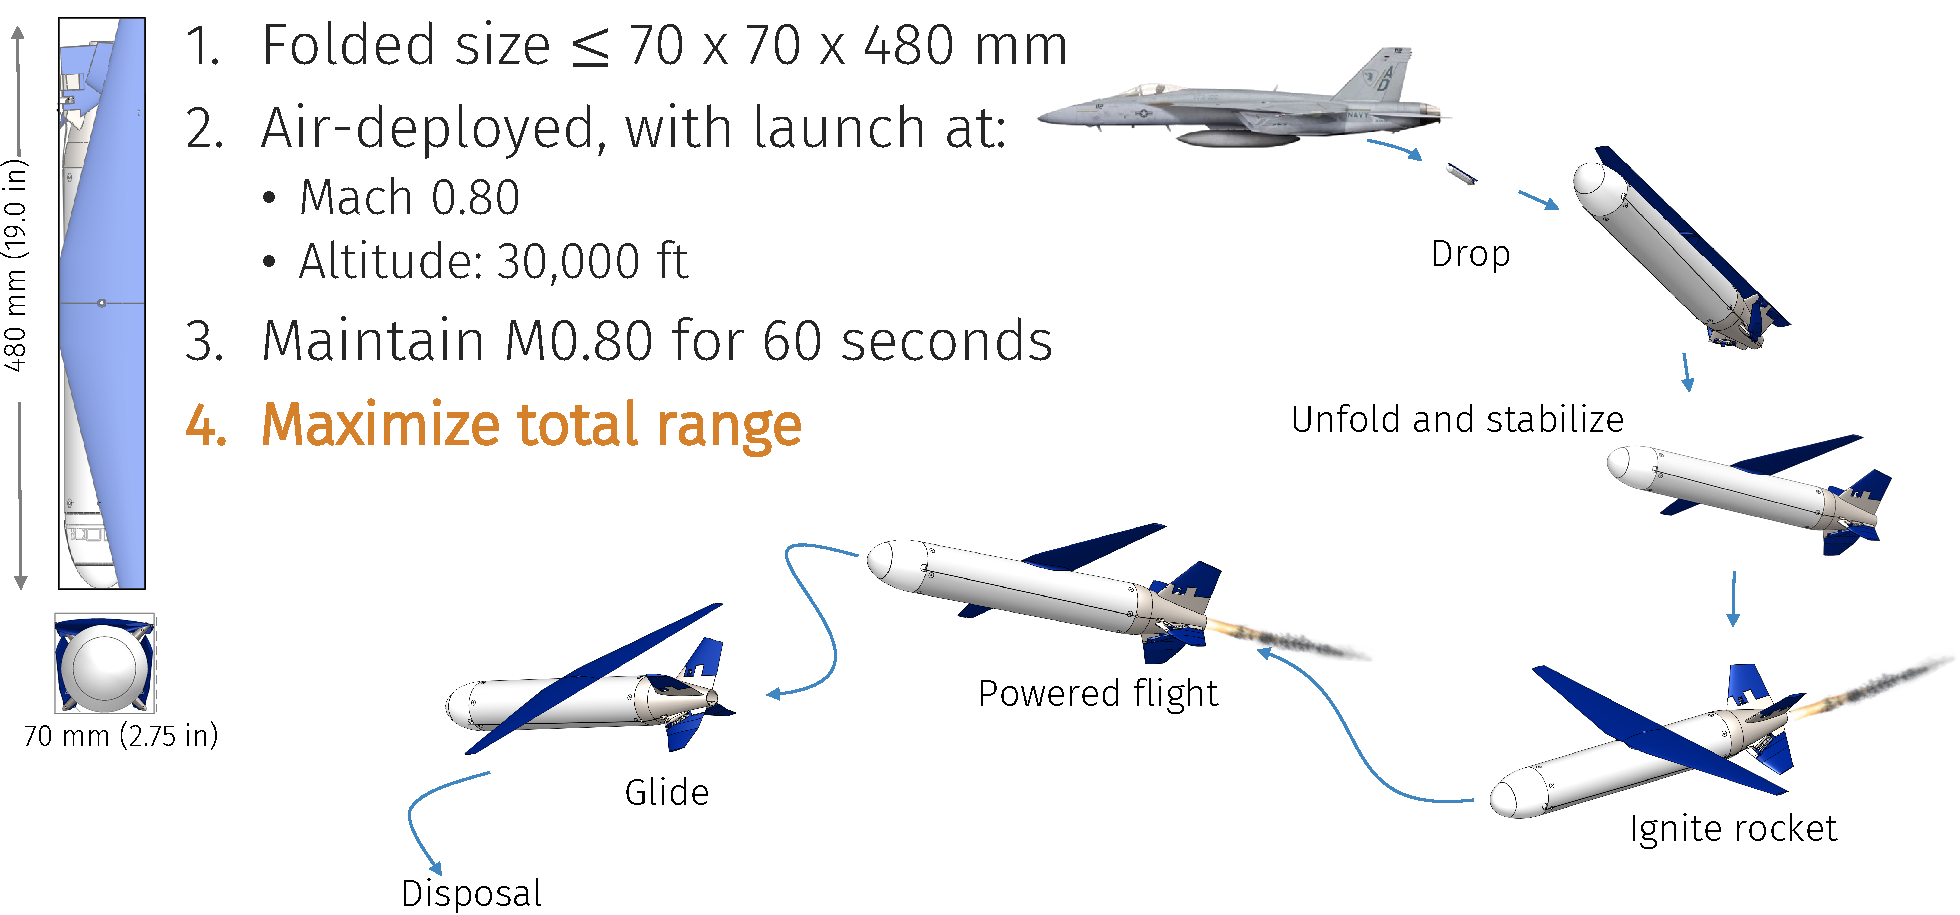
\includegraphics[width=\textwidth]{../figures/firefly_conops-crop.pdf}
    \caption{Concept of operations for the MIT Firefly UAV, adapted from Vernacchia \cite{vernacchia_development_2020}. CAD renders prepared by Julia Gaubatz \cite{gaubatz_design_2024}. F/A-18 image reproduced from McDonnell Douglas.}
    \label{fig:firefly_conops}
\end{figure}

As explained by Vernacchia \cite{vernacchia_development_2020}, Firefly aims to fill a previously-unexplored ``small and fast gap'' in the aircraft design space, with sustained cruise speeds of Mach 0.8 and a gross weight of 2.2 kg\footnote{For comparison: most air vehicles at this size scale are propeller-driven and fly at roughly Mach 0.2 or less. Most air vehicles capable of this sustained speed have gross weights at least an order of magnitude larger.}.

\begin{figure}[h]
    \centering
    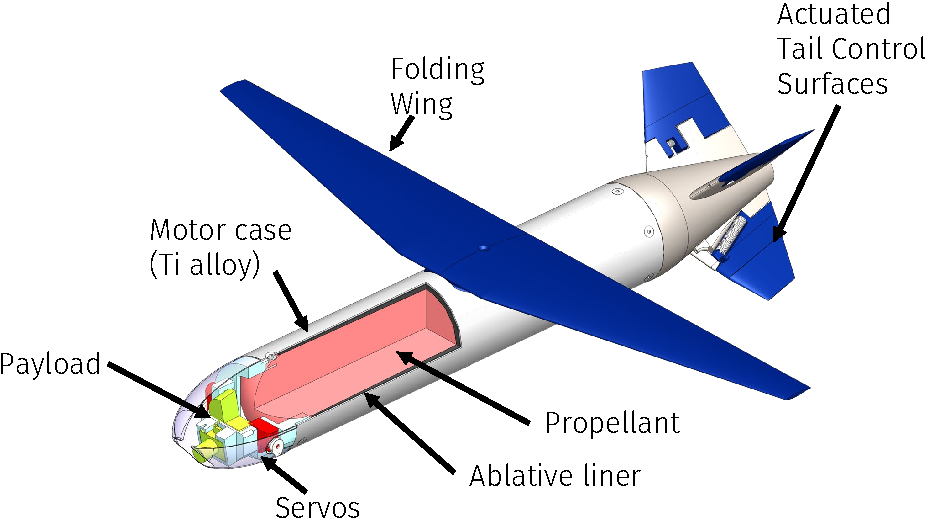
\includegraphics[width=\textwidth]{../figures/firefly_cutout-crop.pdf}
    \caption{Cutout-view of MIT Firefly, showing various unique features. CAD render prepared by Julia Gaubatz \cite{gaubatz_design_2024}.}
    \label{fig:firefly_cutout}
\end{figure}

Before even beginning the computational design process, we can observe some high-level design drivers from first principles. First, the vehicle is relatively insensitive to mass, which contrasts strongly with most aircraft design problems. This is because of a few reasons:
\begin{itemize}[noitemsep]
    \item The vehicle is air-launched at the dash speed and altitude, which means that no additional propulsive energy need be expended to reach this state. Although some of this initial kinetic energy is lost to drag during the initial stabilization transient upon deployment\footnote{and added mass tends to increase the moments of inertia, which slows down the short-period flight dynamics mode}, this is a relatively minor effect.
    \item During the dash phase, the freestream dynamic pressure is extremely high relative to the vehicle's projected area. In fact, were it not for the glide phase, the folding wing shown in Figure \ref{fig:firefly_conops} could be discarded, and body lift alone would be easily produce sufficient aerodynamic lift. Because of where this vehicle operates on the drag polar during the dash phase, the drag force is relatively insensitive to lift, and hence, vehicle weight.
    \item During the glide phase, the vehicle can be trimmed to any preferred airspeed, and naturally, the range-maximizing trajectory will have the aircraft fly at the best-glide speed. The glide ratio is essentially invariant to vehicle mass\footnote{barring some slight Reynolds number effects due to best-glide speed change, which are higher-order effects.}, so the range is also relatively insensitive to vehicle weight.
\end{itemize}

Because of this insensitivity to mass and the focus on total range, one can predict that the major design drivers for Firefly should essentially distill into the following:
\begin{itemize}[noitemsep]
    \item To maximize range during the dash phase: a) pack as much useful propulsive energy into the specified volume as possible, such that this dash phase can be sustained as long as possible and b) reduce drag, even at the expense of lift.
    \item To maximize range during the glide phase: achieve the highest $L/D$ ratio possible.
\end{itemize}

This first-principles design driver calling for the highest-possible volumetric energy storage naturally leads to hydrocarbon fuels\footnote{as opposed to electric batteries}. To achieve reasonable propulsive efficiency at Mach 0.8, the practical propulsion architectures are either a turbine engine or a rocket engine (which may be solid, liquid, or hybrid); tradeoffs are discussed by Vernacchia \cite{vernacchia_development_2020}. In short, a solid rocket engine requires far less ``volume overhead'' to be spent on the engine itself than any other option, especially at this size scale\footnote{Though first-principles physics favor a solid rocket, implementing this comes with some challenges. A particularly interesting one is how to slow down the burn such that the total impulse can be spread across a long enough duration. Vernacchia \cite{vernacchia_development_2020} and Mathesius \cite{mathesius_integrated_2023, mathesius_firefly_2019} explore a mix of clever chemical and physical strategies to achieve this.}. This allows the most possible volume to be spent on energy-rich propellant.

These design drivers also allow one to easily foresee that volume allocations will come at a premium when designing Firefly: expanding the volume available for propellant will inevitably result in fuselage shapes that generate more wave drag at the M0.8 dash condition\footnote{because these higher-volume shapes are blunter, and hence cause a deeper low-pressure spike resulting in stronger shock formation}. This sets the stage for an interesting multidisciplinary design optimization problem, where these coupled relationships can be explored further.

\subsection{MDO Problem Formulation}
\label{sec:firefly-mdo}

The design of Firefly is formulated as a combined vehicle-and-trajectory optimization problem, as these two are inextricably linked. The trajectory is represented via a predetermined number of discrete points in time (roughly $N=200$), which are connected via a direct collocation method\footnote{A introduction to the math representing the dynamics here is given by Kelly \cite{kelly_introduction_2017}.}. This is depicted in Figure \ref{fig:firefly_time_discretization}.

Because the flight physics fundamentally change between dash and glide phases (as the rocket motor no longer produces thrust after this point, and some aerodynamic changes regarding base drag occur), Firefly is inherently a multi-phase dynamics problem. Accordingly, the discretized dynamics are partitioned into two phases. Critically, to maintain $C^1$-continuity (and hence, optimization friendliness), we employ a strategy that we call \emph{stretchy time} that ensures that any given discretization node never crosses this phase boundary, as this would cause a discontinuous change in the problem physics. In this strategy, the time values corresponding to phase transitions (e.g., when rocket motor burnout occurs; when the vehicle contacts the ground and terminates the mission) are free variables in the optimization problem. In contrast, the time values corresponding to intermediate points have their relative spacing within a phase fixed \emph{a priori}. (In this case, this is done with ``cosine-spaced'', also called Chebyshev node, relative positions in time.) Points in time that fall exactly on a phase boundary are included in both phases, with a zero-time-difference collocation constraint that stitches the two phases together; this adds a few degrees of freedom but greatly simplifies indexing.

\begin{figure}[H]
    \centering
    \includesvg[width=0.7\textwidth]{../figures/firefly_time_discretization.svg}
    \caption{``Stretchy time'' time discretization strategy used for the MIT Firefly MDO problem and other multi-phase combined-vehicle-and-dynamics optimization problems.}
    \label{fig:firefly_time_discretization}
\end{figure}

The physics formulation of the optimization problem can be summarized as follows:

\begin{example}
    \textbf{MIT Firefly MDO Problem Formulation}

    \begin{itemize}
        \item \textbf{Objective Function}: Maximize the total mission range, defined as the sum of the dash and glide phases.

        \item \textbf{Design Variables} (in total, 3,910 variables):
        \begin{itemize}
            \item A series of trajectory design variables, including downrange distance, altitude, airspeed, flight path angle, and angle of attack. Note that this parameterization a) is two-dimensional, representing the trajectory in range-altitude space and b) makes a quasi-steady assumption\footnote{using the definition from Drela \cite{drela_flight_2013}}, which essentially assumes that the short-period mode is much faster than the meaningful trajectory dynamics\footnote{Equivalent ways to state this are that we assume the vehicle an instantaneously trim to a desired angle of attack, or that the nondimensionalized angular rates (e.g., $\bar{p}, \bar{q}, \bar{r}$) are very small.}. This quasi-steady assumption does not, however, assume that the vehicle is in force equilibrium at each time point; the ``raw input'' of the control algorithm can be thought of as the angle of attack.

            \item Various other time-dependent variables, such as the control surface deflections, instantaneous fuel mass, chamber pressure, and nozzle exit pressure. These variables dynamically change vehicle mass properties (and hence stability and control) as well as propulsion performance (e.g., specific impulse), causing both to vary at each discrete time point that is analyzed.

            \item The vehicle design itself, which includes:
            \begin{itemize}
                \item Geometric shape variables. The wing and tail geometries are parameterized by a collection of planform variables; airfoils were optimized separately, as the integrated high-dimensional airfoil shape optimization capabilities described in Chapter \ref{chap:physics-informed-ml} were not yet developed at the time of this study. The general fuselage shape topology was fixed \emph{a priori} based on manufacturing considerations detailed by Vernacchia \cite{vernacchia_development_2020}, consisting of an ellipsoidal nose, a cylindrical midsection, and a conical boattail\footnote{Original versions of this problem allowed far more geometric degrees of freedom, such as non-circular fuselages. Research in collaboration with Vernacchia \cite{vernacchia_development_2020} revealed that non-circular fuselages lead to unacceptable solid rocket grain cracking due to the pressure chamber's deformation under high pressure.}. Various dimensions of this fuselage were allowed to vary, such as the fineness ratio of the nose (which has important wave drag implications) and the angle of the boattail. The relative position and incidence of all lifting surfaces was also left free.

                \item Propulsion design variables. These include both chemistry considerations (e.g., the mass fraction of oxamide, a burn rate suppressant) as well as physical parameters (e.g., throat diameter, expansion ratio, ablative liner thicknesses)

                \item Variables giving a detailed component-wise weight and volume breakdowns of the aircraft, which allows satisfaction of implicit structural analysis models, as well as mass properties modeling. This approach allows natural inclusion of components like ballast, which may be needed for acceptable handling qualities.

            \end{itemize}
        \end{itemize}

        \textbf{Constraints} (in total, 8,420 constraints), which are primarily drawn from six interacting disciplinary analyses:
        \begin{itemize}
            \item \textbf{Aerodynamics}: a component-wise buildup of lift, drag, and moment using AeroSandbox's AeroBuildup model, detailed in Section TODO.
            \item \textbf{Stability \& Control}: a linearized flight dynamics modal analysis, which uses stability derivatives computed by directly differentiating the aerodynamics model and constrains the spectral characteristics of the short-period, Dutch roll, and spiral mode dynamics.
            \item \textbf{Structures \& Mass Properties}: weight closure and structural analysis using first-order models, calibrated to test articles for as-built Firefly prototypes.
            \item \textbf{Propulsion}: A 1D nozzle flow analysis (and in later versions, a detailed reacting chemical kinetics model implemented by Mathesius \cite{mathesius_integrated_2023}), which computes the thrust and specific impulse of the rocket motor at each time point.
            \item \textbf{Trajectory / Dynamics}: A direct collocation method, which enforces the equations of motion at each time point, as well as the boundary conditions at the start and end of each phase.
            \item \textbf{Volume accounting / Packaging}: A series of geometric constraints that ensure that the vehicle fits within the specified stowage volume\footnote{A notable constraint is that the trailing edge of the main wing cannot be swept backwards for packaging reasons, as the wing is a single rotating piece. A two-part jackknife wing (e.g., \emph{MIT Perdix} \cite{tao_design_2012}) was considered, but we find that the propellant volume penalty of the added mechanisms thickness does not outweigh the aerodynamic gain.}, as well as that the propellant grain fits within the pressure chamber.
        \end{itemize}

    \end{itemize}

\end{example}

Because every analysis module used in this Firefly design problem is compatible with a code transformations paradigm, formulating this as an ``all-in-one'' optimization problem within a simultaneous analysis and design (SAND) architecture is straightforward \cite{haftka_simultaneous_1985, martins_multidisciplinary_2013}. This overall MDO problem architecture is loosely depicted in Figure \ref{fig:sand}, where most constraints are formulated implicitly. (This contrasts with nested approaches to closure, which is shown in Figure \ref{fig:nested})

\begin{figure}[h]
    \centering
    \includesvg[width=\textwidth]{../figures/sand.svg}
    \caption{Schematic of the simultaneous analysis and design (SAND) architecture used for the MIT Firefly MDO problem.}
    \label{fig:sand}
\end{figure}

The Firefly MDO problem is relatively high-dimensional, with 3,910 decision variables and 8,420 constraints, many of which are nonlinear and nonconvex. Evaluation of the problem constraints and objective take the bulk of the runtime; in particular, the $N=200$ workbook-style aerodynamic analyses (one for each discrete point along the trajectory) performed at each iteration tend to be the most computationally expensive elements. Nevertheless, using AeroSandbox with CasADi and IPOPT backends, the problem converges to a solution in a wall-clock runtime of just 6.9 seconds on a laptop\footnote{with a Ryzen 5800H CPU}. Equally notable is the fact that this problem can be implemented using only 613 lines of Firefly-specific Python code, which is possible because many of the constituent analyses use general-purpose aerospace physics models that are optionally provided by AeroSandbox. This speed and conciseness allows the user to rapidly and interactively explore the design space, as well as to perform sensitivity analyses and trade studies.

\subsection{Results}

The point results of the Firefly design optimization problem yields the vehicle design shown in the CAD render of Figure \ref{fig:firefly_cutout}. However, one of the first compelling framework-level observations that was made during this case study was how useful it is to be able to immediately visualize the aircraft geometry within seconds of solving the optimization problem. As quipped by aircraft designer Bob Liebeck\footnote{personal correspondence}, ``you can tell a lot about an airplane by whether it passes the TLAR: `That Looks About Right' .'' Therefore, this case study was the motivation for building the AeroSandbox aircraft geometry stack, a code-transformations-compatible library that allows for rapid visualization of new designs. The raw outputs of this geometry stack are shown in Figure \ref{fig:firefly_geometry}, and the resemblance between this initial OML render from AeroSandbox and the final CAD render of Figure \ref{fig:firefly_cutout} is apparent.

\begin{figure}[h]
    \centering
    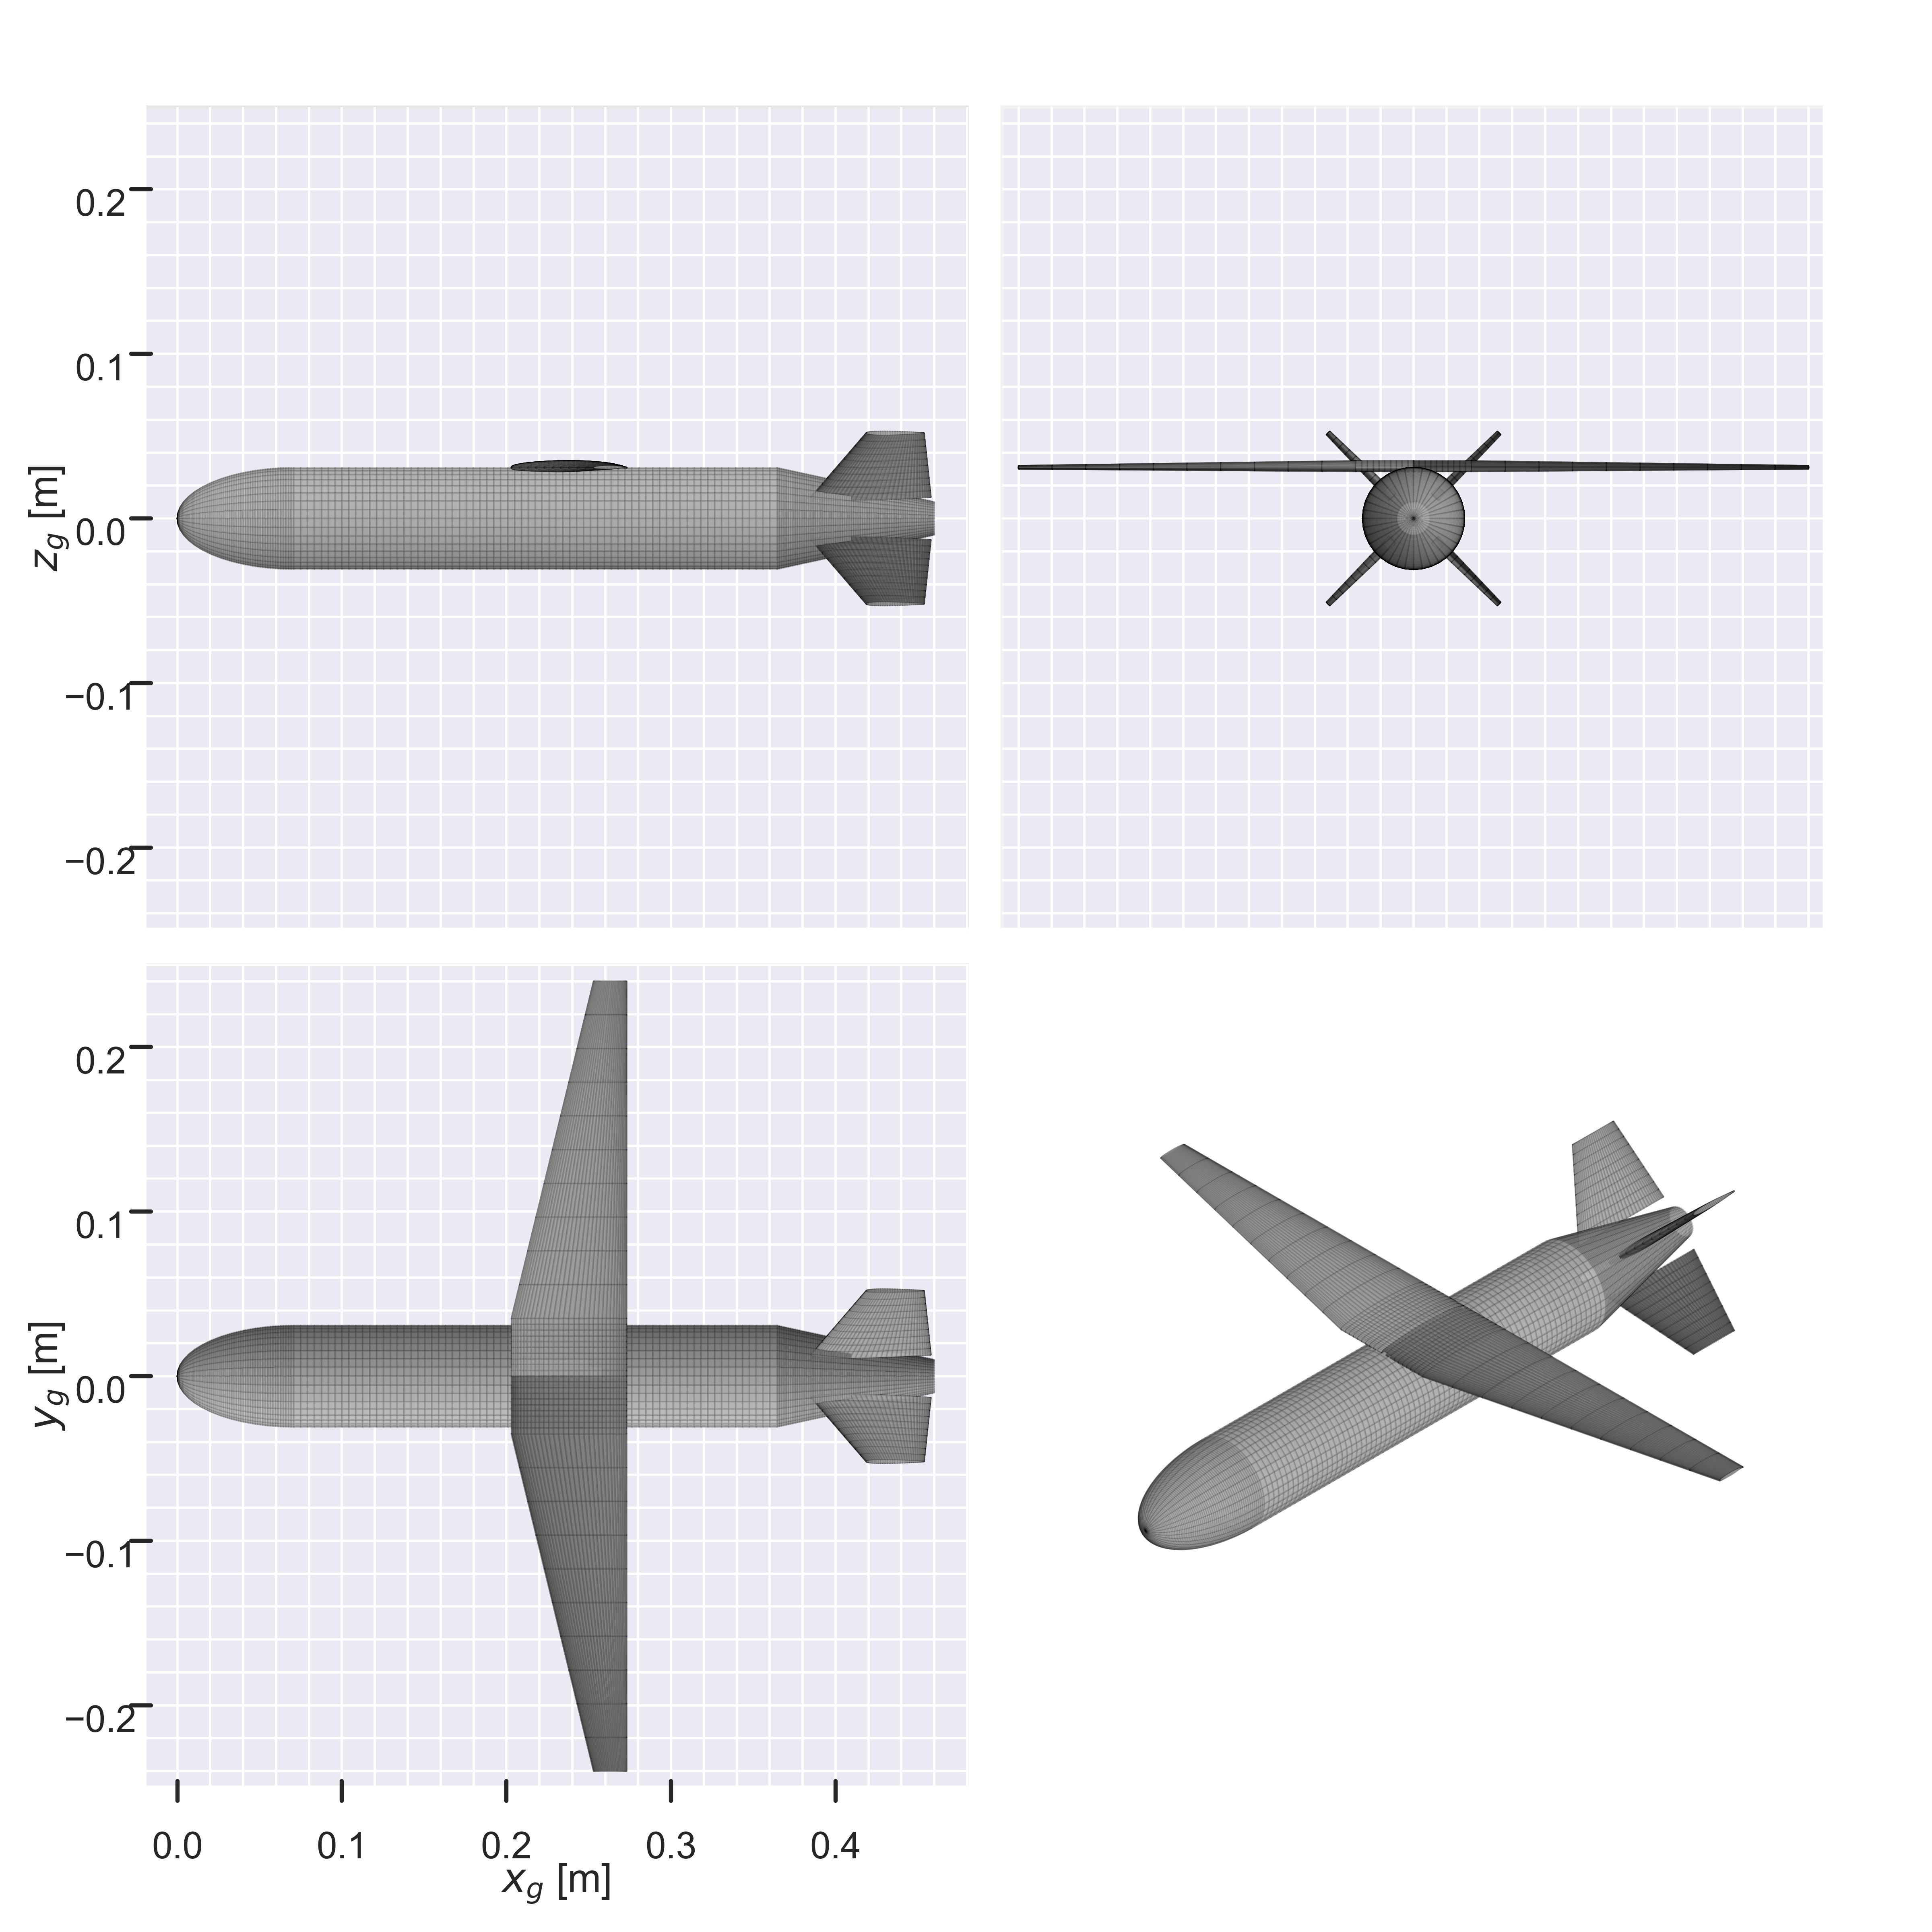
\includegraphics[width=\textwidth]{../figures/firefly_geometry.png}
    \caption{Raw user-facing output of the AeroSandbox geometry stack for the MIT Firefly UAV.}
    \label{fig:firefly_geometry}
\end{figure}

Internal volume and mass accounting of various components at the design point are shown in Table \ref{tab:firefly_mass}, with values that were later validated against as-built prototypes.

\begin{table}
    \centering
    \caption{Mass and volume accounting of various components of the MIT Firefly UAV, at the point design resulting from the formulation given in Section \ref{sec:firefly-mdo}. Mixed units are the result of preferences by various project stakeholders.}
    \label{tab:firefly_mass}
    \begin{tblr}{
        colspec={@{} l m{4cm} m{4cm} m {4cm} @{}},
        row{1}={font=\bfseries},
        column{1}={font=\bfseries},
    }
        \toprule
        Component         & Internal volume [$\rm in^3$] (Percentage) & Mass [gram] (Percentage of gross) & $x_g$ of CG, relative to nose datum [mm] \\
        \midrule
        Fuel (at gross)   & 38.8 (54.2\%)                             & 1019 (42.7\%)                     & 321                                      \\
        Battery           & 9.8 (13.7\%)                              & 322 (13.5\%)                      & 58                                       \\
        Case              & 7.9 (11.0\%)                              & 579 (24.2\%)                      & 230                                      \\
        Liner             & 5.7 (7.9\%)                               & 136 (5.7\%)                       & 321                                      \\
        Mechanisms        & 4.1 (5.8\%)                               & 20 (0.8\%)                        & 447                                      \\
        Payload           & 2.5 (3.5\%)                               & 100 (4.2\%)                       & 78                                       \\
        Avionics          & 2.1 (2.9\%)                               & 75 (3.1\%)                        & 100                                      \\
        Nozzle            & 0.7 (1.0\%)                               & 15 (0.6\%)                        & 447                                      \\
        Wing              & -                                         & 53 (2.2\%)                        & 188                                      \\
        Tails             & -                                         & 70 (2.9\%)                        & 436                                      \\
        \midrule
        Total (gross)     & 71.5 (100\%)                              & 2389 (100\%)                      & 248                                      \\
        Total (zero-fuel) & 71.5 (100\%)                              & 1370 (57.3\%)                     & 195                                      \\
        \bottomrule
    \end{tblr}
\end{table}

The resulting trajectory, which was simultaneously optimized with the vehicle, is shown in Figure \ref{fig:firefly_trajectory}. Here, a number of notable findings can be observed:

\begin{enumerate}
    \item The vehicle is capable of achieving far greater operational range than had been initially anticipated. Initial hand-calculated estimates based on an assumed vehicle design and trajectory had estimated that total ranges of 70 kilometers might be possible\footnote{As a rough napkin-math calculation, a 60-second dash at Mach 0.8, followed by a glide at a $L/D$ of 7 (owing to the low Reynolds number and assumed low-aspect-ratio wing) yields a range of 70 km.}, while the combined optimization result yields ranges of over 230 kilometers.
    \item This massive range increase is achieved partially by co-optimization of various aircraft subsystems, like making aeropropulsive trades on the fuselage shape, which influences dash range. This was expected, and is typical of the power of an MDO approach. However, the majority of the range increase was due to the unique trajectory that the optimizer found, which is shown in Figure \ref{fig:firefly_trajectory}. Here, the vehicle rapidly climbs to a very high altitude—well into the stratosphere—before gliding down. This allows the vehicle to take advantage of two clever effects:
    \begin{enumerate}
        \item The arcing trajectory effectively lets the vehicle use gravitational potential energy as a battery. Because of this, the burn duration of the solid rocket motor can be much shorter for a given impulse, as excess energy goes somewhere useful (i.e., altitude) rather than somewhere wasteful (i.e., wave drag). By allowing a shorter burn, the propellant chemistry can be tweaked to use less burn rate suppressant (oxamide), which increases the specific impulse of the motor. This dynamics-propulsion coupling was not foreseen.
        \item By climbing high, the \emph{indicated} airspeed of the vehicle is much lower while holding the Mach 0.8 constraint. This reduces the dash-phase drag penalty of having a large, high-aspect-ratio, high-$L/D$ wing. By increasing the wingspan, the glide-phase $L/D$ becomes much larger, which gives a large range increase. In addition to enhancing the glide ratio, climbing high also simply increases the glide range directly. This inter-phase aerodynamic trade was also unexpected.
    \end{enumerate}
\end{enumerate}

\begin{figure}[h]
    \centering
    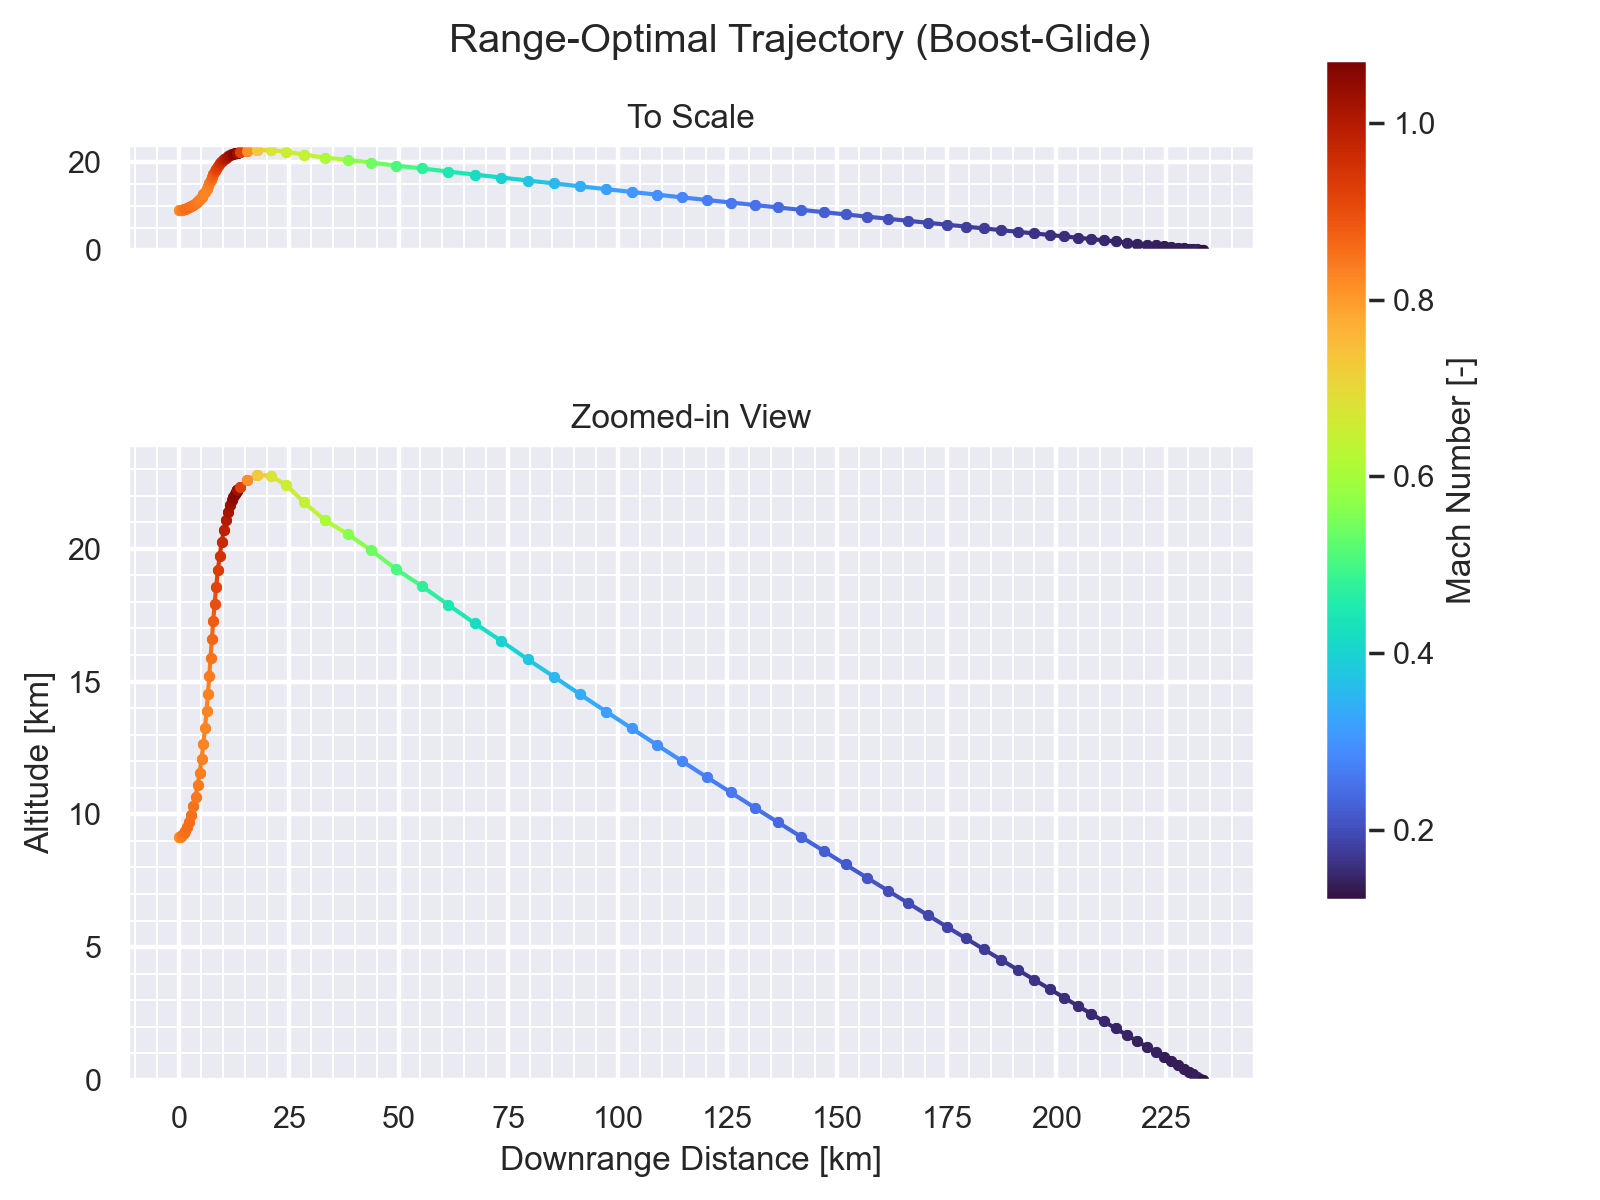
\includegraphics[width=\textwidth]{../figures/BAE-2022-06-17-Peter/ppt/media/image7.png}
    \caption{Trajectory that maximizes vehicle total range, resulting from the combined vehicle-and-trajectory MDO problem formulation given in Section \ref{sec:firefly-mdo}.}
    \label{fig:firefly_trajectory}
\end{figure}

This trajectory, while unexpected, indeed satisfies requirements, and its discovery was only possible through the use of a combined vehicle-and-trajectory optimization approach. This is a key benefit of the code transformations paradigm: the ability to rapidly explore the design space and discover unexpected interactions between subsystems.

\subsection{Design Space Sweeps}
\label{sec:firefly_sweeps}

As discussed further in Appendix \ref{appendix:rules-of-thumb}, the value of an engineering design optimization framework is not just in the point design, but also in the insight that it provides. An early example of this observation was made during the Firefly design study, where the optimizer was used to explore the tradeoffs between optimizing for total range (dash + glide) vs. optimizing for dash range alone. In AeroSandbox, this can be easily performed, all without leaving a procedural coding style with the following syntax:

\begin{enumerate}[noitemsep]
    \item Replace the objective function with a simple linear combination of the total and dash ranges, with a weighting factor $w \in [0, 1]$. Define $w$ as an optimization parameter, using:
    \begin{minted}[highlightlines={5}]{python}
        import aerosandbox as asb
        opti = asb.Opti()  # Initialize an optimization environment
        ... # Define the rest of the optimization problem

        w = opti.parameter()
    \end{minted}

    \item Instead of solving the problem with \mintinline{python}{opti.solve()}, solve it with:

    \begin{minted}[highlightlines={1}]{python}
        sols = opti.solve_sweep({w: np.linspace(0, 1)})
    \end{minted}

\end{enumerate}

Using this syntax, the user can convert a point design optimization problem to a design sweep (i.e., looking at a set of optimal points, as some parameter is varied) in just two lines of code.

For this particular case study, the results of such a sweep are shown in Figure \ref{fig:firefly_pareto}. Clearly, though designs can be optimized purely for total range or only for dash range, there are many opportunities where a small sacrifice in one can yield large gains in the other—this may be of interest to the practical designer. Likewise, it shows how the vehicle resulting from the optimizer (in the lower-right) differs dramatically from the original napkin-math ``mental model'' that was used for initial performance estimates. Because this initial design did not use an arcing trajectory, the wing area (and hence, glide-phase $L/D$) was quite limited.

Charts like these can be crucial in high-level conceptual decision-making, where an entire family of aircraft can be depicted in a single chart. The results of this design sweep take a few minutes to compute in serial, but parallelization across cores or computers can allow this to be presented to the user in seconds.

\begin{figure}[h]
    \centering
    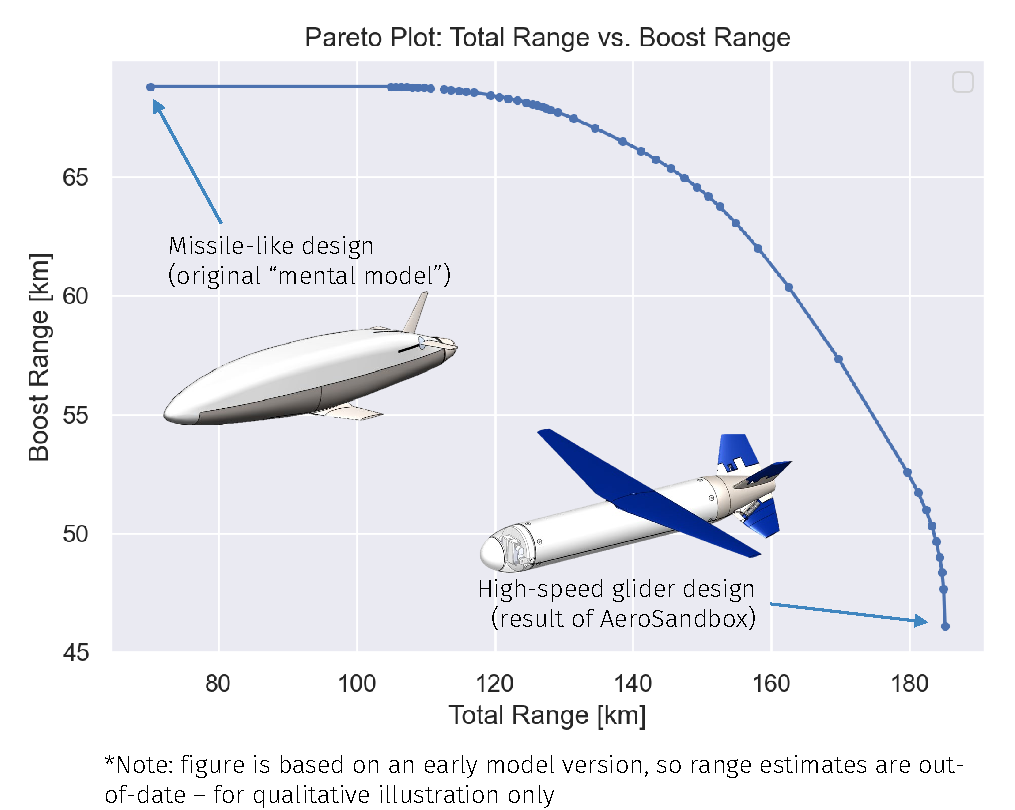
\includegraphics[width=\textwidth]{../figures/firefly_pareto-crop.pdf}
    \caption{Pareto front of the MIT Firefly UAV design space, showing the tradeoff between total range and dash range. Each point represents both a unique vehicle design and trajectory.}
    \label{fig:firefly_pareto}
\end{figure}

\subsection{Supporting Flight Test}

Finally, AeroSandbox-based performance calculations were used to support the Firefly air vehicle through manufacturing, first flight, and a controls characterization flight test campaign \cite{gaubatz_design_2024}. Media from this flight test campaign are given in Figure \ref{fig:firefly_flight_test}. The vehicle was found to be stable and controllable, and the flight test data was used to validate the aerodynamics model used in the optimization problem.

This experience also motivated the development of purpose-built aircraft flight dynamics tools within AeroSandbox, which can be used to directly reconstruct and visualize the flight trajectory of the vehicle. This can be performed for both computationally-optimized trajectories as well as from actual measured flight test data, allowing both design and post-flight analysis to be conducted in the same environment for easy model validation. An example of this is shown in Figure \ref{fig:firefly_flight_render}, which shows the trajectory of Firefly's first flight test, reconstructed and visualized in AeroSandbox. Notably, during this flight test the vehicle was air-dropped from a quadcopter\footnote{with further details given by Gaubatz \cite{gaubatz_design_2024}}, which can be seen in the steep vertical trajectory at the beginning of the flight as the vehicle stabilizes.

This experience emphasized how useful it is to have an MDO tool that can switch between analysis (e.g., only closure, no optimization) and design modes, as discussed in the birds-eye view of optimization shown in Figure \ref{fig:birds_eye_view}. An MDO tool, if built correctly, has the potential to follow the vehicle through its lifecycle similar to a digital twin, providing value from the conceptual design phase through to flight test.

\begin{figure}[h]
    \centering
    \begin{subfigure}[b]{0.5\textwidth}
        \centering
        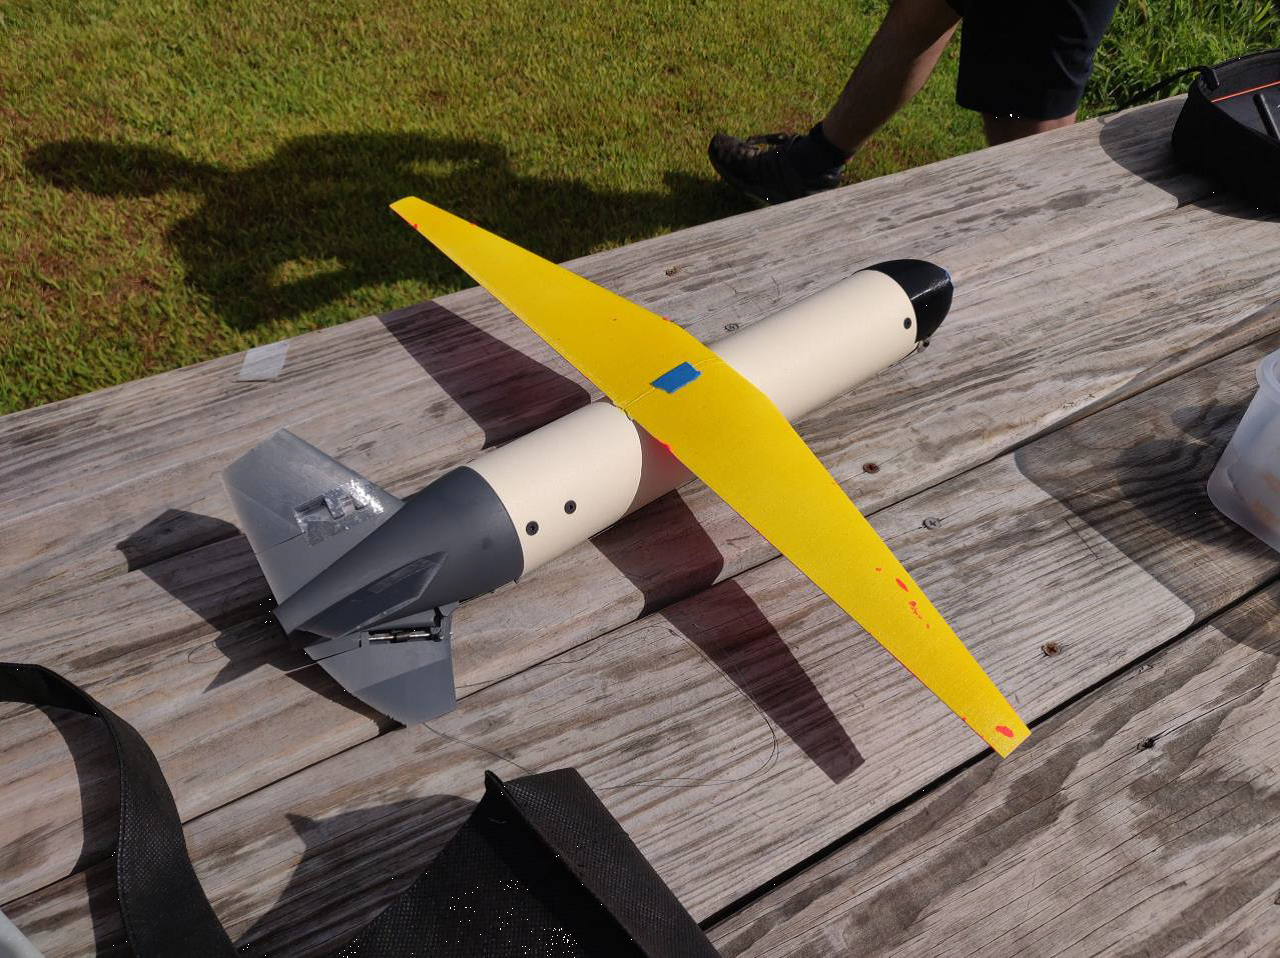
\includegraphics[width=\textwidth]{../figures/firefly_flight_1.png}
        \caption{As-built Firefly air vehicle, prepared for first flight.}
    \end{subfigure}
    \hfill
    \begin{subfigure}[b]{0.432\textwidth}
        \centering
        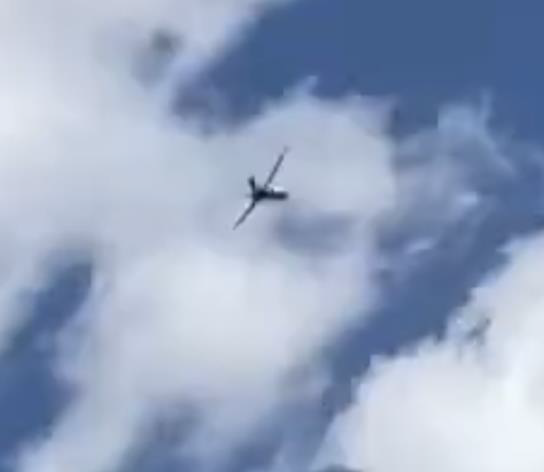
\includegraphics[width=\textwidth]{../figures/firefly_flight_2.png}
        \caption{Photograph of the MIT Firefly air vehicle in-flight, cruising at roughly 40 m/s.}
    \end{subfigure}
    \caption{Photos of the MIT Firefly prototype. Vehicle constructed by Julia Gaubatz \cite{gaubatz_design_2024}.}
    \label{fig:firefly_flight_test}
\end{figure}

\begin{figure}[h]
    \centering
    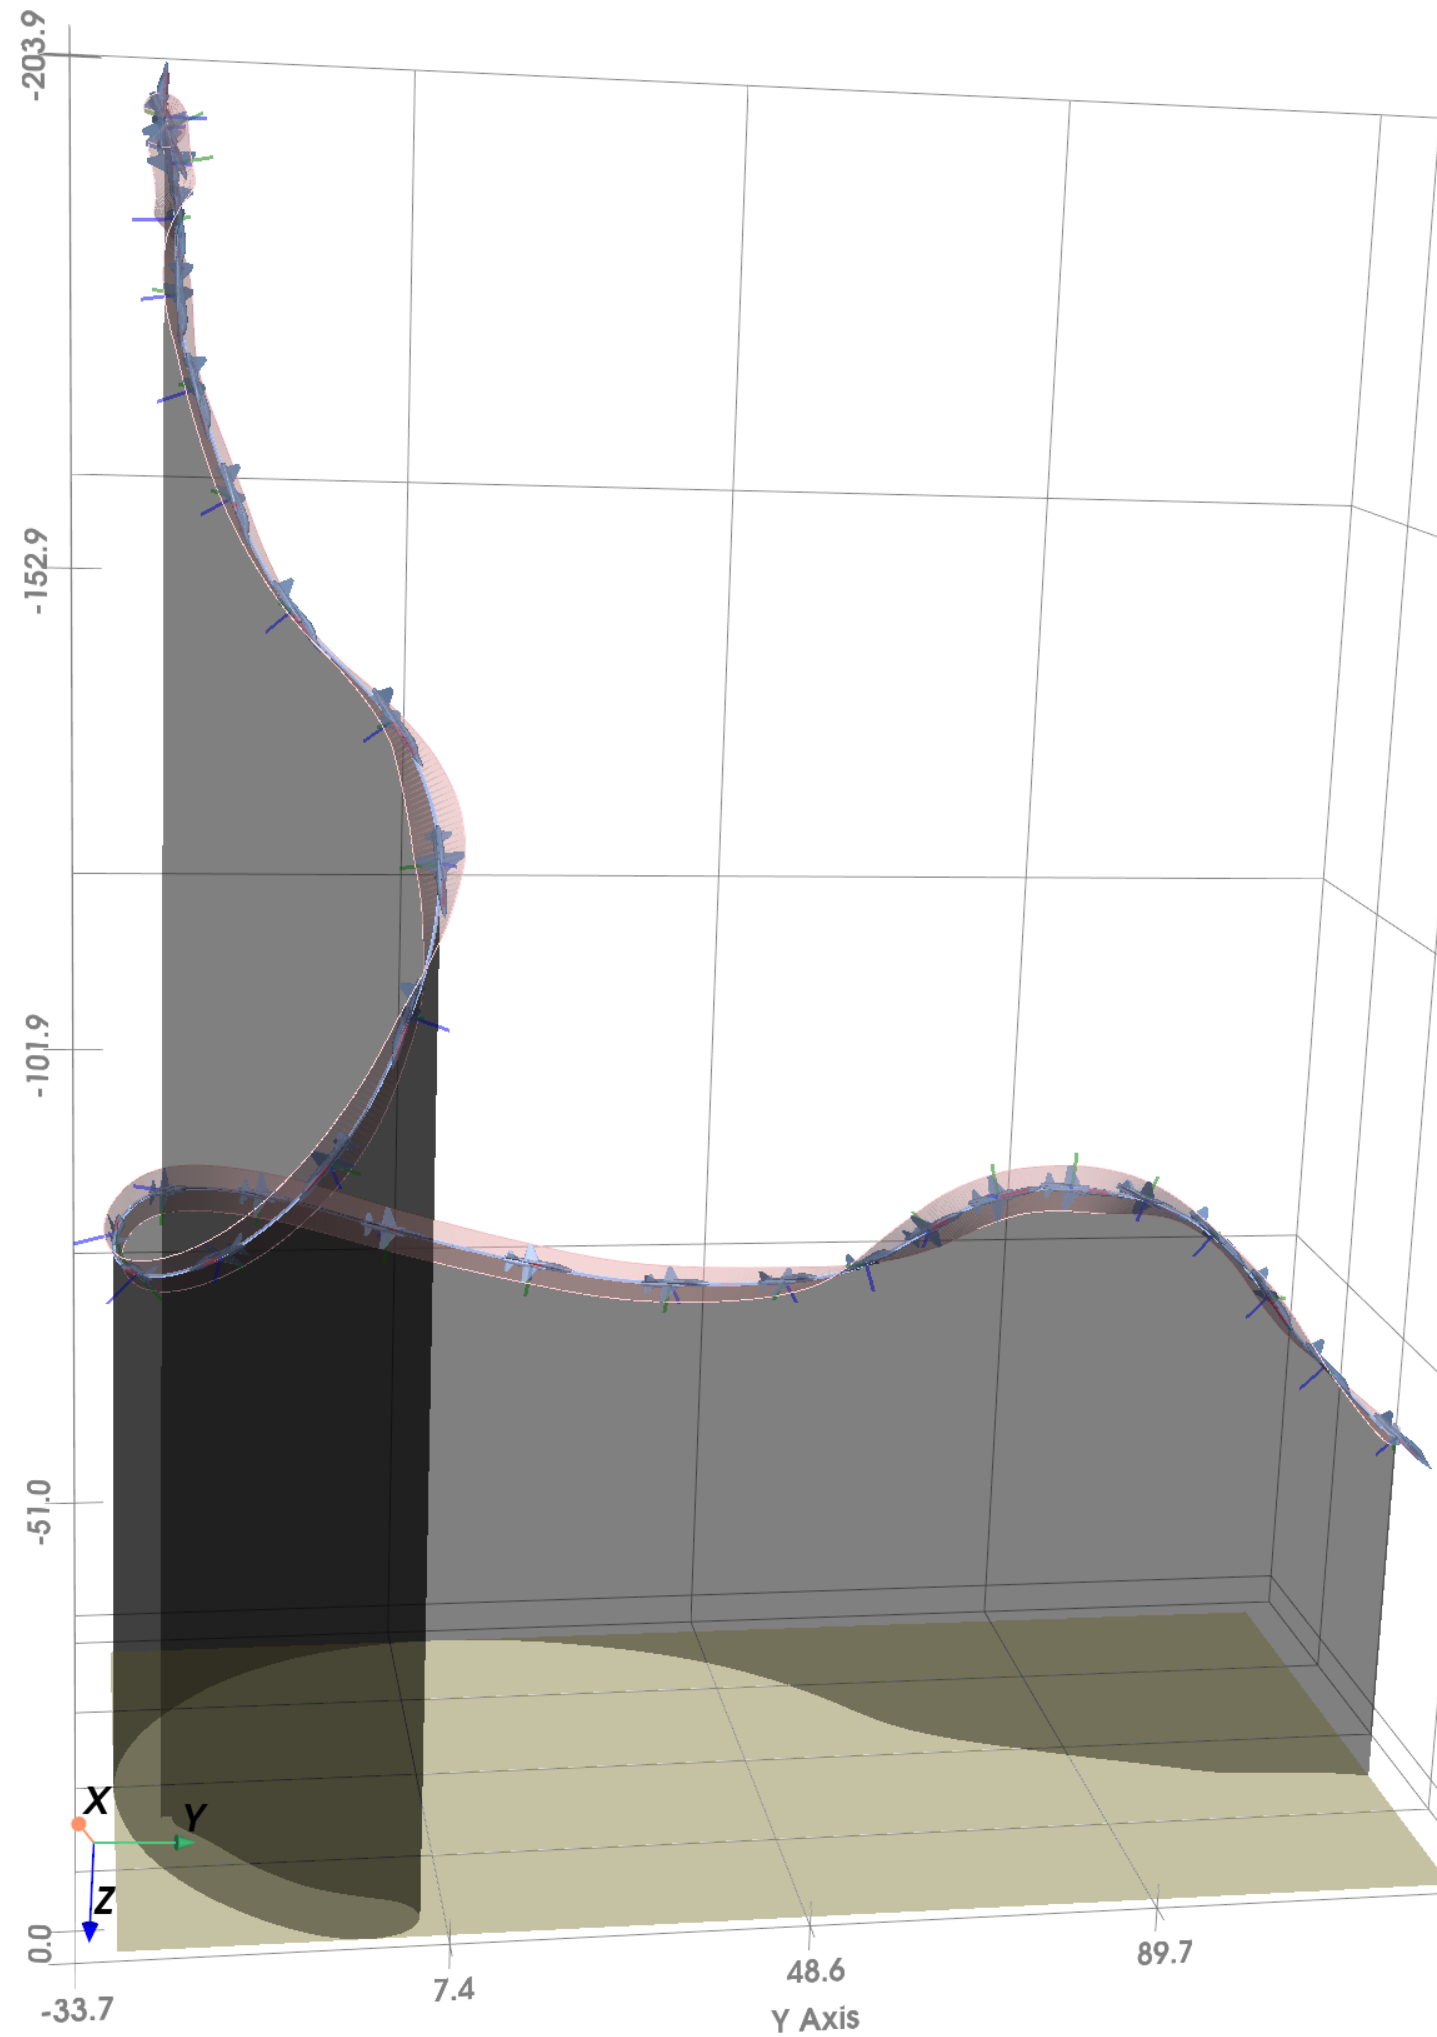
\includegraphics[width=0.95\textwidth,trim={0 0.2in 0 0.8in}]{../figures/firefly_flight_render.png}
    \caption{Flown trajectory of the first flight of MIT Firefly, reconstructed and visualized in the AeroSandbox dynamics stack. Vehicle is drawn using a generic aircraft model and at roughly 30x scale, which allows easier visualization of vehicle orientation. Flight test was air-dropped from a quadrotor, with the stabilization period visible at the beginning of the trajectory.}
    \label{fig:firefly_flight_render}
\end{figure}


\section{MIT Dawn (Electra.aero SACOS) Solar-Electric HALE Aircraft}
\label{sec:dawn}

\subsection{Problem Overview}

A second aircraft design case study that contributed heavily to the development of AeroSandbox was \emph{MIT Dawn}, a solar-electric high-altitude long-endurance (HALE) aircraft. This aircraft development program was later transferred to industry partner Electra.aero and incorporated into the Stratospheric Airborne Climate Observatory System (SACOS) program, where the aircraft has achieved first flight and is undergoing further development.

The Dawn aircraft development program began as a set of solution-agnostic requirements aimed at supporting a climate science mission \cite{dewald_multidisciplinary_2023, sharpe_optimization_2021, avery_16_}. This science mission, conceived by an atmospheric chemistry research group at Harvard\footnote{The Anderson Research Group, under the direction of Professor James Anderson.}, aims to take atmospheric chemistry measurements of various free radicals in the stratosphere, which must be performed in-situ over long durations. This information would allow scientists to further reduce the uncertainty about the rate of climate change, which could allow for more precise and effective policy measures to be implemented \cite{dykema_feasibility_2023}. A variety of aircraft design requirements were developed and negotiated with the science team, with the major driving ones as follows:

\begin{itemize}[noitemsep]
    \item \textbf{Payload}: 30 kg science package, with 500 W electrical power draw during daylight hours and 150 W at night
    \item \textbf{Altitude}: sustained flight at 60,000 ft. MSL (18.3 km) or above
    \item \textbf{Endurance}: 6 weeks continuous flight during July–August
    \item \textbf{Station-keeping}: with the ability to maneuver and maintain position over any location in the continental United States, in 95th-percentile winds
\end{itemize}

We initially approached this aircraft design problem by exploring a wide range of conceptual solutions. In addition to a solar aircraft, the team considered a superpressure balloon (E.g., Google Loon), a powered airship, a rotating fleet of conventional aircraft (e.g., Aurora Flight Sciences Orion), long-endurance hydrogen aircraft (E.g., AeroVironment Global Observer), ground-tethered balloons, and numerous others\footnote{Even some nuclear-powered aircraft concepts were briefly considered.}. Each of these had a rapid feasibility analysis conducted in AeroSandbox based on first-principles physics, similar in scope to the SimpleAC problem given in Section \ref{sec:simpleac}. This capability to quickly pose sizing studies allowed these proposed concepts to be matured to the point where a meaningful and fair comparison\footnote{i.e., a true apples-to-apples comparison, where an \emph{optimized} variant of concept A is compared to an \emph{optimized} variant of concept B} could be made; ultimately, a solar-powered HALE aircraft was selected, with further reasoning available in Sharpe et al. \cite{sharpe_optimization_2021}.

\subsection{Vehicle Overview}

The MIT Dawn aircraft is a sailplane-like configuration, as shown in Figure \ref{fig:dawn_overview}. On the outboard sections of the wing, two small all-moving aerodynamic surfaces are mounted on booms extending from the wing trailing edge. These two unique surfaces, called \emph{tailerons}, are used for roll control and aeroelastic stabilization; further details on these surfaces are given in recent work by Sharpe, Ulker, and Drela \cite{sharpe_tailerons_2023}. Propulsion is provided by two propellers, which are wing-mounted and driven by electric motors. The payload is held in a separate pod, mounted with a truss beneath the main wing to allow for propeller clearance.

\begin{figure}[h]
    \centering
    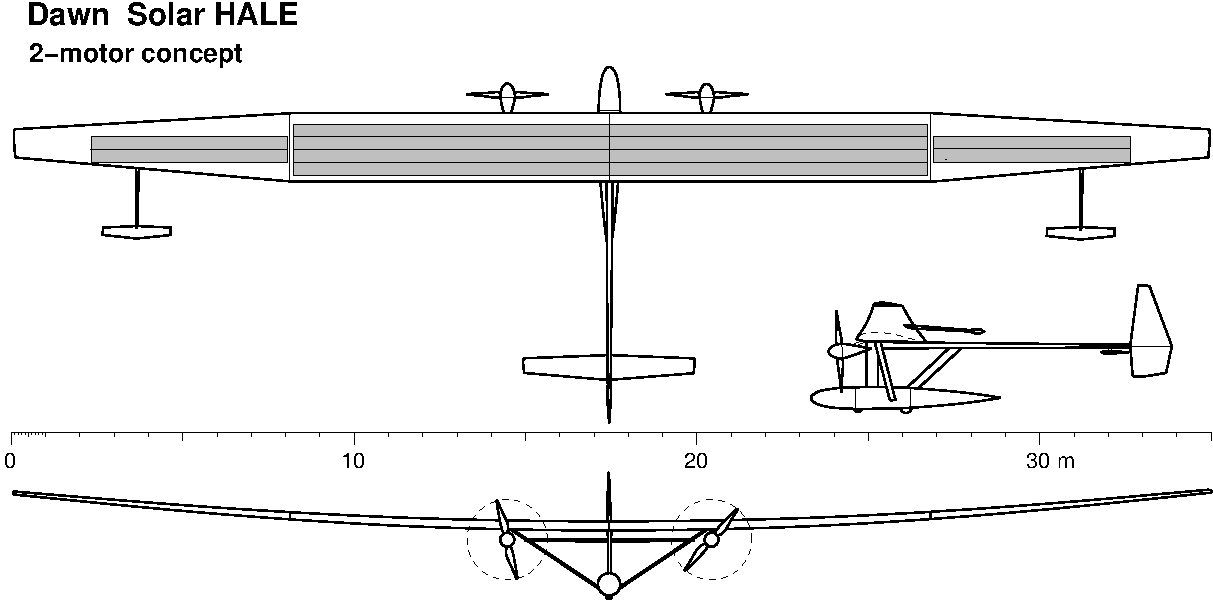
\includegraphics[width=\textwidth]{../figures/dawn1_3view.pdf}
    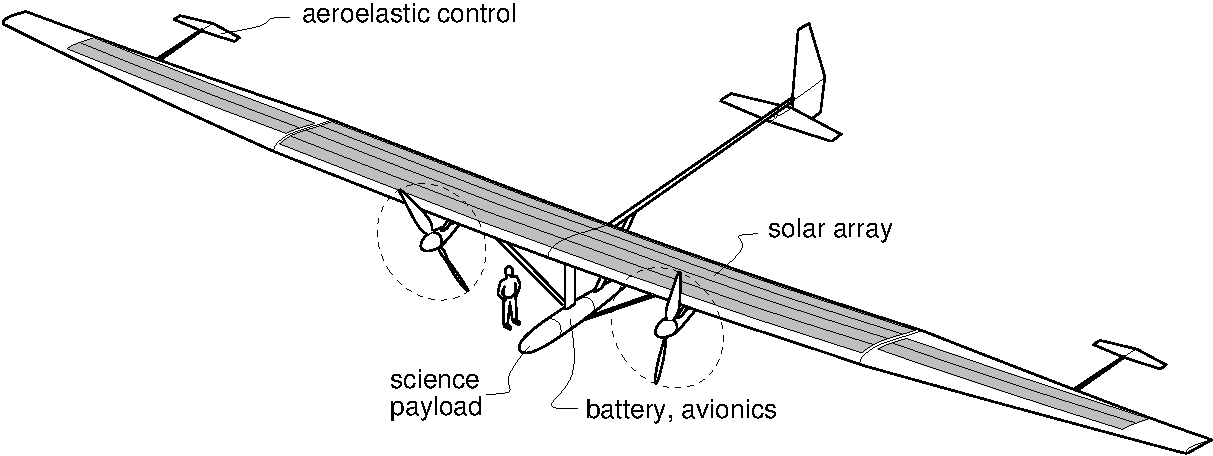
\includegraphics[width=\textwidth]{../figures/dawn1b.pdf}
    \caption{Basic aircraft configuration, approximate scale, and major components of the MIT Dawn solar-electric HALE aircraft. Exact aircraft dimensions vary depending on technology assumptions. Figure illustrated by Mark Drela.}
    \label{fig:dawn_overview}
\end{figure}


The aircraft is powered by a series of solar cells, which are mounted on the main wing in spanwise strings\footnote{This arrangement keeps each cell within the string at similar solar incidence angles, which makes them impedence-matched and results in fewer power-point-tracking losses.}. Approximately 80\% of the wing's surface is covered with solar cells, with this solar area fraction limited by the curvature tolerance of cells when mounted near the leading edge. Various solar cells were considered, with the baseline design using Sunpower C60 cells with a cell-level efficiency of 24.3\%\footnote{Further modifications to the actual cell energy generation based on line-of-sight airmass absorption, atmospheric refraction, backscattering, surface albedo, covering transparency, and other effects are also considered.}.

Overnight flight is supported by a large battery, which is mounted in the pod. Due to the project's experimental nature, relatively advanced battery technologies are assumed; the baseline design assumes a cell-level battery specific energy of 450 Wh/kg\footnote{This is already achievable by a few commercially-available cells at the time of writing, such as the Amprius Technologies silicon-anode cells and Sion Power lithium-sulfur cells. These cells use exotic chemistries that come with some (acceptable) design considerations; further discussion is available in Sharpe et al. \cite{sharpe_optimization_2021}.}. Pack-level specific energy is slightly lower, as we assume the cells form 89\% of the overall pack mass; this is based on as-built weights from the prior Aurora Odysseus solar aircraft.

The aircraft cruises at an altitude of between 60,000 and 65,000 ft. MSL, which is above the tropopause at most latitudes and seasons. This essentially nullifies the possibility of cloud cover, reduces exposure to aeroelastically-risky gusts, and reduces steady wind speeds\footnote{At most points in the latitude-seasonality space, this altitude is above the jet stream.} (reducing the required cruise speed for stationkeeping). An interesting mission strategy that is used here (which was discovered using the MDO process described in Section \ref{sec:dawn-mdo}) is the idea of \emph{altitude cycling}: during the day, the aircraft recharges its batteries until approximately 3 p.m. local solar time, after which it uses the excess solar power to climb higher. During the night, the vehicle glides lower (though never below 60,000 ft.), which reduces power draw and required battery mass. This essentially allows the vehicle to use gravitational potential energy as a battery, which is a similar clever combined-vehicle-and-trajectory optimization exploit that was found in the Firefly design.

Table \ref{tab:dawn_overview} summarizes various key parameters of the aircraft in its cruise condition, and a high-level mass budget is given in Figure \ref{fig:dawn_mass_budget}. From this figure, the difficulty of designing a solar-electric HALE aircraft with overnight endurance is apparent: the battery is nearly half the gross weight of the aircraft, and the payload mass fraction is a mere 8\%.

\begin{table}[h]
    \centering
    \caption{Key specifications for the point design corresponding to the baseline mission. Reproduced from Sharpe et al. \cite{sharpe_optimization_2021}.}
    \label{tab:dawn_overview}
    \begin{tblr}{
        colspec={@{} X X @{}},
        row{1} = {font=\bfseries},
    }
        \toprule
        Figure of Merit         & Value at Design Point                                 \\
        \midrule
        Gross weight            & 375 kg                                                \\
        Wingspan                & 39.9 m                                                \\
        Wing aspect ratio       & 23.4                                                  \\
        Wing area               & 67.9 m$^2$                                            \\
        Wing loading            & 54.2 Pa                                               \\
        Cruise airspeed (true)  & 30.4 m/s                                              \\
        Altitude                & 18.7 km nighttime and peaking at 19.7 km on Aug. 31st \\
        Total power output      & Peak net battery draw: 5.07 kW                        \\
        Battery capacity        & 75.4 kWh                                              \\
        Wing Reynolds number    & $383\times 10^3$ ($c_\text{ref}=\bar{c}$)             \\
        Cruise lift coefficient & 1.11                                                  \\
        Cruise $L/D$ Ratio      & 30.8                                                  \\
        \bottomrule
    \end{tblr}
\end{table}

\begin{figure}[h]
    \centering
    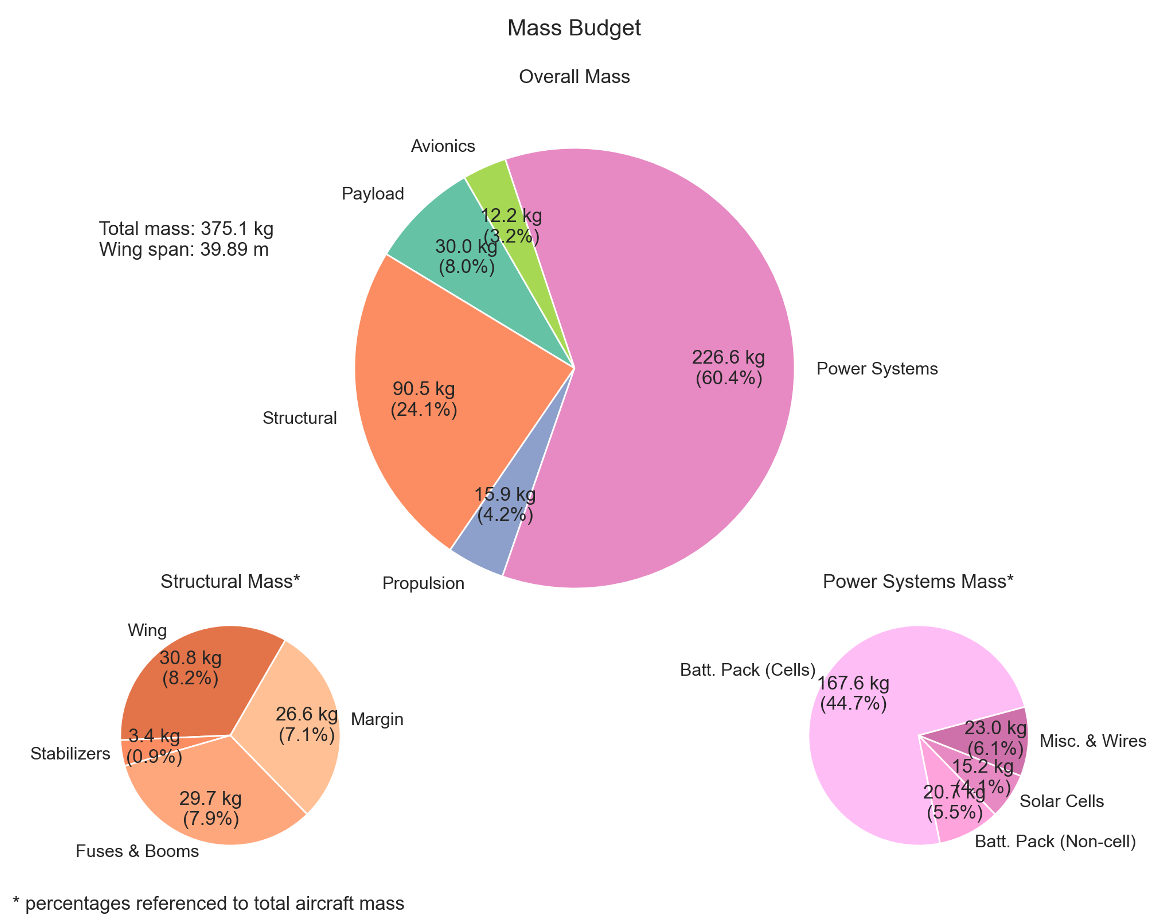
\includegraphics[width=\textwidth]{../figures/dawnfigures/Mass_breakdown_baseline.png}
    \caption{High-level mass budget for the MIT Dawn solar-electric HALE aircraft. Large pie chart shows total breakdown, with the smaller pie charts showing subsystem-level breakdowns for the structural and power systems components. Reproduced from Sharpe et al. \cite{sharpe_optimization_2021}.}
    \label{fig:dawn_mass_budget}
\end{figure}

\subsection{MDO Problem Formulation}
\label{sec:dawn-mdo}

\begin{attrib}
    This subsection includes content from the author's contributions to prior work by Sharpe, Dewald, and Hansman \cite{sharpe_optimization_2021}.
\end{attrib}

Just as with the Firefly design problem, the MIT Dawn design problem was formulated as a combined vehicle-and-trajectory optimization problem. The trajectory represents a 24-hour cycle, beginning and ending at solar noon. This periodic interval is of interest here because of the inherent challenge of \emph{diurnal energy closure}: a solar aircraft must be capable of ending any given 24-hour period within the mission envelope with more potential energy (in the forms of battery charge state and altitude) than it started with\footnote{Some additional energy margin must be included here, for robustness. In this study, we add energy generation margin by effectively decreasing the solar insolation in all conditions by a flat 5\% knockdown.}.

While sufficient energy generation is key to ensuring energy closure, energy storage also constrains the design space. The aircraft's battery must be sized so that its charge state remains within allowable bounds\footnote{A maximum allowable battery depth-of-discharge of 85\% was assumed.} - given the time-varying solar insolation and unsteady power draws (from the propulsion system, payload, and avionics), evaluating the feasibility of this constraint for a given solution becomes nontrivial. Furthermore, one would expect that a system with cyclic power injections might be optimally operated using a cyclic strategy; and indeed this is observed via altitude cycling under some assumptions.

To incorporate this trajectory information into the optimization problem, the flight equations of motion are once again embedded via a direct collocation method, with trapezoidal quadrature. A convergence study was performed for the solar aircraft design problem in order to determine an appropriate temporal resolution. Testing indicated that grid-independence was reliably achieved at a temporal resolution of 150 collocation points uniformly spaced over a 24-hour interval; therefore, this was the discretization resolution used in all further studies.

The physics formulation of the optimization problem can be summarized as follows:

\begin{example}
    \textbf{MIT Dawn MDO Problem Formulation}

    \begin{itemize}
        \item \textbf{Objective Function}: Minimize the wingspan of the aircraft. This choice of objective is somewhat unusual, and it is chosen as a proxy for measuring an important technical risk. Historically, the most common failure modes of solar aircraft have been aerostructural in nature\footnote{Example solar aircraft with at least one documented in-flight aeroelastic failure include NASA Helios, Google/Titan Solara 50, Facebook Aquila, and Airbus Zephyr.}, and wingspan is a good first-order measure of how severe these aeroelastic challenges will be. In addition, previous development programs for large solar aircraft (such as Aurora’s Odysseus, at 74 meters wingspan) have attributed significant operational challenges (e.g., runway width, transport, support equipment, and cost) directly to wingspan.

        \item \textbf{Design Variables} (in total, roughly 2,500 variables)
        \begin{itemize}
            \item Trajectory design variables, with a similar 2D parameterization as in Section \ref{sec:firefly-mdo}. Unlike the Firefly problem, however, the steady assumption is taken further, and instantaneous force equilibrium is assumed at each time point; in this way, the flight dynamics essentially become an energy accounting problem, with all velocity derivative terms dropped. In other words, the ``raw input'' of the control algorithm can be thought of as velocity. This neglects direct simulation of \emph{both} the short-period and phugoid flight dynamics modes, which are assumed to be much faster than the problem dynamics of interest (i.e., diurnal changes in energy injection from solar power).

            \item Other time-dependent variables, such as the throttle setting, control surface deflections, and battery state of charge. Time-dependent cross-discipline coupling variables, like overall vehicle net power are also added.

            \item The vehicle design itself, which includes:
            \begin{itemize}
                \item Geometric shape variables, with a similar general parameterization methodology as the Firefly MDO setup of Section \ref{sec:firefly-mdo}.

                \item Propulsion sizing, including battery capacity, propeller diameters, motor voltage constants, and rated power of various electrical components

                \item Detailed structural design variables, such as the wing rib count and payload truss sizing. Never-exceed speeds and ultimate load factors during gusts are also optimized, allowing the creation of a $V-N$ flight envelope with appropriate margins. As in Section \ref{sec:firefly-mdo}, component-wise weights are also included as variables that are satisfied by implicit structural analysis models.
            \end{itemize}
        \end{itemize}

        \item \textbf{Constraints} (in total, roughly 4,000 constraints), drawn directly and indirectly from several interacting disciplinary analyses, with the major ones as follows:
        \begin{itemize}

            \item \textbf{Aerodynamics}: a component-wise buildup of lift, drag, and moment using AeroSandbox's AeroBuildup model, detailed in Section TODO. A nonlinear lifting line method and a vortex lattice method were also included as alternate options used to validate the buildup model. Optimization solutions typically differ by only a few percent between models, which implies good cross-validation. This is unsurprising, as a solar airplane represents a near-ideal case for typical theoretical assumptions for 3D aerodynamics (high aspect ratios, well-separated lifting surfaces).

            \item \textbf{Stability \& Control}: Static stability is verified through a workbook-style buildup of the location of the aircraft's neutral point, with static margin set as 20\% of mean aerodynamic chord\footnote{This static margin, which is a hair high for a high-$L/D$ aircraft, is intended to mitigate risk. Fixing a too-aft CG during detailed design usually costs more weight than fixing a too-forward CG, due to differences in available moment arms.}.

            \item \textbf{Structures \& Mass Properties}: Primary structure weights are physics-based where possible. For example, the wing spar weight and carbon fiber layup schedule are the result of an Euler-Bernoulli beam model with both bending and torsion\footnote{For speed, this is broken out as a separate optimization sub-problem, which is pre-computed for a wide range of spans and load distributions. A closed-form solution is then used as the ``online'' model during the broader MDO problem.}. Secondary structures are generally modeled using empirical statistical models. For example, many wing secondary structures are modeled based on data from the \emph{MIT Daedalus} project \cite{cruz_weight_1989, cruz_structural_1989, langford_feasibility_1986}, with a 30\% markup to mitigate operational challenges documented by the Daedalus team \cite{langford_daedalus_1989}.

            \item \textbf{Propulsion}: A propeller model based on dynamic disc actuator theory with viscous correction factors is implemented \cite{unified_propellers}. Viscous correction factors are calibrated using the blade-element code QPROP with sectional airfoil data from XFoil \cite{drela_xfoil_1989, qprop}.

            \item \textbf{Trajectory / Dynamics}: A direct collocation method, which enforces the equations of motion at each time point. Path constraints, such as battery state of charge limits, altitude minimums, and airspeed minimums (i.e., station-keeping) are also added. In addition, periodicity constraints are added, which ensure energy closure over the 24-hour cycle.

            \item To support station-keeping constraints, a probabilistic model of both steady winds and gusts was developed using data from the ECMWF ERA5 reanalysis dataset \cite{era5}. The model is a function of latitude, longitude, and day of year, which allows global mapping of the feasible mission space.

        \end{itemize}

    \end{itemize}

\end{example}

Further details on the MIT Dawn MDO problem formulation and constituent models are available in Sharpe et al. \cite{sharpe_optimization_2021}. As with the Firefly problem, the Dawn problem is implemented in AeroSandbox using a SAND architecture; Figure \ref{fig:dawn_xdsm} shows the data flow within the MDO process in extended design structure matrix (XDSM) format \cite{xdsm}.

\begin{figure}[h]
    \centering
    \begin{adjustbox}{width=\textwidth,center,trim={3.5in 0 0.25in 0}}
        \setstretch{1.0}
        
%%% Preamble Requirements %%%
% \usepackage{geometry}
% \usepackage{amsfonts}
% \usepackage{amsmath}
% \usepackage{amssymb}
% \usepackage{tikz}

% Optional packages such as sfmath set through python interface
% \usepackage{sfmath}

 \usetikzlibrary{arrows,chains,positioning,scopes,shapes.geometric,shapes.misc,shadows}

%%% End Preamble Requirements %%%

% Define all the styles used to produce XDSMs for MDO

% Tableau 20 color palette, taken from
% https://jrnold.github.io/ggthemes/reference/tableau_color_pal.html
% we use the lighter variants here with 80% opacity
% Blue
\definecolor{red}{HTML}{A0CBE8}
% Orange
\definecolor{orange}{HTML}{FFBE7D}
% Cyan
\definecolor{cyan}{HTML}{86BCB6}
% Green
\definecolor{green}{HTML}{8CD17D}
% Yellow
\definecolor{yellow}{HTML}{F1CE63}
% Salmon
\definecolor{salmon}{HTML}{FF9D9A}

\tikzstyle{every node}=[font=\sffamily,align=center]

\newcommand{\fillOpacity}{80}

% Component shapes
\newcommand{\compShape}{rectangle}
\newcommand{\groupShape}{chamfered rectangle}
\newcommand{\procShape}{rounded rectangle}

% Colors
\newcommand{\explicitColor}{green}
\newcommand{\implicitColor}{salmon}
\newcommand{\optimizationColor}{red} % also used by DOE

% Component types
\tikzstyle{Optimization} = [\procShape,draw,fill=\optimizationColor!\fillOpacity,inner sep=6pt,minimum height=1cm,text badly centered]
\tikzstyle{MDA} = [\procShape,draw,fill=orange!\fillOpacity,inner sep=6pt,minimum height=1cm,text badly centered]
\tikzstyle{DOE} = [\procShape,draw,fill=\optimizationColor!\fillOpacity,inner sep=6pt,minimum height=1cm,text badly centered]
\tikzstyle{SubOptimization} = [\groupShape,draw,fill=\optimizationColor!\fillOpacity,inner sep=6pt,minimum height=1cm,text badly centered]
\tikzstyle{Group} = [\groupShape,draw,fill=\explicitColor!\fillOpacity,inner sep=6pt,minimum height=1cm,text badly centered]
\tikzstyle{ImplicitGroup} = [\groupShape,draw,fill=\implicitColor!\fillOpacity,inner sep=6pt,minimum height=1cm,text badly centered]
\tikzstyle{Function} = [\compShape,draw,fill=\explicitColor!\fillOpacity,inner sep=6pt,minimum height=1cm,text badly centered]
\tikzstyle{ImplicitFunction} = [\compShape,draw,fill=\implicitColor!\fillOpacity,inner sep=6pt,minimum height=1cm,text badly centered]
\tikzstyle{Metamodel} = [\compShape,draw,fill=yellow!\fillOpacity,inner sep=6pt,minimum height=1cm,text badly centered]

%% A simple command to give the repeated structure look for components and data
\tikzstyle{stack} = [double copy shadow={shadow xshift=.75ex, shadow yshift=-.75ex}]
%% A simple command to fade components and data, e.g. demonstrating a sequence of steps in an animation
\tikzstyle{faded} = [draw=black!10,fill=white,text opacity=0.2]

%% Simple fading commands for the lines
\tikzstyle{fadeddata} = [color=black!20]
\tikzstyle{fadedprocess} = [color=black!50]

% Data types
\newcommand{\dataRightAngle}{105}
\newcommand{\dataLeftAngle}{75}

\tikzstyle{DataInter} = [trapezium,trapezium left angle=\dataLeftAngle,trapezium right angle=\dataRightAngle,draw,fill=black!10]
\tikzstyle{DataIO} = [trapezium,trapezium left angle=\dataLeftAngle,trapezium right angle=\dataRightAngle,draw,fill=white]

% Edges
\tikzstyle{DataLine} = [color=black!40,line width=5pt,line cap=rect]
\tikzstyle{ProcessHV} = [-,line width=1pt,to path={-| (\tikztotarget)}]
\tikzstyle{ProcessHVA} = [->,line width=1pt,to path={-| (\tikztotarget)}]
\tikzstyle{ProcessTip} = [-,line width=1pt]
\tikzstyle{ProcessTipA} = [->, line width=1pt]
\tikzstyle{FadedProcessHV} = [-,line width=1pt,to path={-| (\tikztotarget)},color=black!30]
\tikzstyle{FadedProcessHVA} = [->,line width=1pt,to path={-| (\tikztotarget)},color=black!30]
\tikzstyle{FadedProcessTip} = [-,line width=1pt,color=black!30]
\tikzstyle{FadedProcessTipA} = [->, line width=1pt,color=black!30]

% Matrix options
\tikzstyle{MatrixSetup} = [row sep=3mm, column sep=2mm]

% Declare a background layer for showing node connections
\pgfdeclarelayer{data}
\pgfdeclarelayer{process}
\pgfsetlayers{data,process,main}

% A new command to split the component text over multiple lines

\newcommand{\MultilineComponent}[2]
{
	\begin{minipage}{#1}
	\begin{center}
		#2
	\end{center}
	\end{minipage}
}

\newcommand{\TwolineComponent}[3]
{
	\begin{minipage}{#1}
	\begin{center}
		#2 \linebreak #3
	\end{center}
	\end{minipage}
}

\newcommand{\ThreelineComponent}[4]
{
	\begin{minipage}{#1}
	\begin{center}
		#2 \linebreak #3 \linebreak #4
	\end{center}
	\end{minipage}
}

% A new command to split the component text over multiple columns
\newcommand{\MultiColumnComponent}[5]
{
	\begin{minipage}{#1}
	\begin{center}
	#2 \linebreak #3
	\end{center}
	\begin{minipage}{0.49\textwidth}
	\begin{center}
	#4
	\end{center}
	\end{minipage}
	\begin{minipage}{0.49\textwidth}
	\begin{center}
	#5
	\end{center}
	\end{minipage}
	\end{minipage}
}

\def\arraystretch{1.3}

\begin{tikzpicture}

\matrix[MatrixSetup]{
%Row 0
&
\node [DataIO] (output_opt) {$\begin{array}{c}\text{Parameters}\end{array}$};&
&
&
&
&
&
&
&
\\
%Row 1
\node [DataIO] (left_output_opt) {$\begin{array}{c}\text{Optimal} \\ \text{A/C \& Traj.}\end{array}$};&
\node [Optimization] (opt) {$\begin{array}{c}\text{Optimizer:} \\ \text{IPOPT}\end{array}$};&
\node [DataInter] (opt-atmo) {$\begin{array}{c}\text{Traj.}\end{array}$};&
\node [DataInter] (opt-aero) {$\begin{array}{c}\text{A/C geom.,} \\ \text{$\alpha, \delta$}\end{array}$};&
\node [DataInter] (opt-stab) {$\begin{array}{c}\text{A/C geom.}\end{array}$};&
\node [DataInter] (opt-prop) {$\begin{array}{c}\text{Prop} \\ \text{Sizing}\end{array}$};&
\node [DataInter] (opt-power) {$\begin{array}{c}\text{Pow. Sys.} \\ \text{Sizing}\end{array}$};&
\node [DataInter] (opt-struct) {$\begin{array}{c}\text{A/C geom.,} \\ \text{$W_{total}$}\end{array}$};&
\node [DataInter] (opt-dyn) {$\begin{array}{c}\text{Traj.,} \\ \text{$W_{total}$}\end{array}$};&
\\
%Row 2
&
&
\node [Function] (atmo) {$\begin{array}{c}\text{Atmosphere}\end{array}$};&
\node [DataInter] (atmo-aero) {$\rho, \nu$};&
&
\node [DataInter] (atmo-prop) {$\rho, \nu$};&
&
&
\node [DataInter] (atmo-dyn) {$\begin{array}{c}\text{Winds}\end{array}$};&
\\
%Row 3
&
\node [DataInter] (aero-opt) {$\begin{array}{c}\text{$\mathcal{R}(\Gamma)$} \\ \text{(for implicit} \\ \text{solvers)}\end{array}$};&
&
\node [Function] (aero) {$\begin{array}{c}\text{Aerodynamics}\end{array}$};&
\node [DataInter] (aero-stab) {$M$};&
&
&
\node [DataInter] (aero-struct) {$L_{max}$};&
\node [DataInter] (aero-dyn) {$L, D$};&
\\
%Row 4
&
\node [DataInter] (stab-opt) {$\mathcal{R}(q, x_{sm})$};&
&
&
\node [Function] (stab) {$\begin{array}{c}\text{Stability}\end{array}$};&
&
&
&
&
\\
%Row 5
&
&
&
&
&
\node [Function] (prop) {$\begin{array}{c}\text{Propulsion}\end{array}$};&
\node [DataInter] (prop-power) {$P, P_{max}$};&
\node [DataInter] (prop-struct) {$W_{prop}$};&
\node [DataInter] (prop-dyn) {$T$};&
\\
%Row 6
&
\node [DataInter] (power-opt) {$\mathcal{R}(\int P_{net} dt = E_{batt})$};&
&
&
&
&
\node [Function] (power) {$\begin{array}{c}\text{Power} \\ \text{Systems}\end{array}$};&
\node [DataInter] (power-struct) {$W_{psys}$};&
\node [DataInter] (power-dyn) {$P_{net}$};&
\\
%Row 7
&
\node [DataInter] (struct-opt) {$\begin{array}{c}\text{$\mathcal{R}(W_{total} = \sum W_i)$} \\ \text{$\mathcal{R}(\text{Beam eqns.})$}\end{array}$};&
&
&
&
&
&
\node [Function] (struct) {$\begin{array}{c}\text{Structures} \\ \text{\& Weights}\end{array}$};&
&
\\
%Row 8
&
\node [DataInter] (dyn-opt) {$\mathcal{R}(F = ma)$};&
&
&
&
&
&
&
\node [Function] (dyn) {$\begin{array}{c}\text{Dynamics}\end{array}$};&
\\
%Row 9
&
&
&
&
&
&
&
&
&
\\
};

% XDSM process chains


\begin{pgfonlayer}{data}
\path
% Horizontal edges
(opt) edge [DataLine] (opt-atmo)
(opt) edge [DataLine] (opt-aero)
(opt) edge [DataLine] (opt-stab)
(opt) edge [DataLine] (opt-prop)
(opt) edge [DataLine] (opt-power)
(opt) edge [DataLine] (opt-struct)
(opt) edge [DataLine] (opt-dyn)
(atmo) edge [DataLine] (atmo-aero)
(atmo) edge [DataLine] (atmo-prop)
(atmo) edge [DataLine] (atmo-dyn)
(aero) edge [DataLine] (aero-stab)
(aero) edge [DataLine] (aero-struct)
(aero) edge [DataLine] (aero-dyn)
(prop) edge [DataLine] (prop-power)
(prop) edge [DataLine] (prop-dyn)
(prop) edge [DataLine] (prop-struct)
(power) edge [DataLine] (power-struct)
(power) edge [DataLine] (power-dyn)
(aero) edge [DataLine] (aero-opt)
(stab) edge [DataLine] (stab-opt)
(power) edge [DataLine] (power-opt)
(struct) edge [DataLine] (struct-opt)
(dyn) edge [DataLine] (dyn-opt)
(opt) edge [DataLine] (left_output_opt)
% Vertical edges
(opt-atmo) edge [DataLine] (atmo)
(opt-aero) edge [DataLine] (aero)
(opt-stab) edge [DataLine] (stab)
(opt-prop) edge [DataLine] (prop)
(opt-power) edge [DataLine] (power)
(opt-struct) edge [DataLine] (struct)
(opt-dyn) edge [DataLine] (dyn)
(atmo-aero) edge [DataLine] (aero)
(atmo-prop) edge [DataLine] (prop)
(atmo-dyn) edge [DataLine] (dyn)
(aero-stab) edge [DataLine] (stab)
(aero-struct) edge [DataLine] (struct)
(aero-dyn) edge [DataLine] (dyn)
(prop-power) edge [DataLine] (power)
(prop-dyn) edge [DataLine] (dyn)
(prop-struct) edge [DataLine] (struct)
(power-struct) edge [DataLine] (struct)
(power-dyn) edge [DataLine] (dyn)
(aero-opt) edge [DataLine] (opt)
(stab-opt) edge [DataLine] (opt)
(power-opt) edge [DataLine] (opt)
(struct-opt) edge [DataLine] (opt)
(dyn-opt) edge [DataLine] (opt)
(opt) edge [DataLine] (output_opt);
\end{pgfonlayer}

\end{tikzpicture}

    \end{adjustbox}
    \caption{Extended Design Structure Matrix (XDSM) representation of the MIT Dawn solar-electric HALE aircraft design optimization problem. Reproduced from Sharpe et al. \cite{sharpe_optimization_2021}.}
    \label{fig:dawn_xdsm}
\end{figure}

\subsection{Results and Framework Lessons}

The result of the optimization process described in Section \ref{sec:dawn-mdo} is the point design summarized in Table \ref{tab:dawn_overview} Figures \ref{fig:dawn_mass_budget}. The point design estimate produced using AeroSandbox was then further refined in collaboration with Electra.aero, leading to the successful construction and first flight of a full-scale demonstrator aircraft, as shown in Figure \ref{fig:dawn_flight}.

\begin{figure}[h]
    \centering
    \includegraphics[width=\textwidth]{../figures/dawn_flight.jpg}
    \caption{Photograph of the Dawn One solar-electric HALE aircraft lifting off during its first flight test, in September 2022. Reproduced from Electra.aero \cite{electra_dawn_flight}.}
    \label{fig:dawn_flight}
\end{figure}

As with the Firefly design, however, many of the valuable lessons learned from the development of this tool were not only from the point design, but also from the trade studies one can quickly assess using this framework.

\subsubsection*{Rapid Performance Sweeps}

As an example of this, a key early question during the design was ``How does the required wingspan vary with latitude and seasonality?'' To answer this, we designed 2,400 unique aircraft (a $60\times40$ grid in seasonality-latitude space), each the result of solving a unique instance of the MDO problem described in Section \ref{sec:dawn-mdo}. With parallelization on a high-performance computing cluster (HPC), computing these results took several minutes, effectively allowing this question to be answered real-time in a meeting with major stakeholders.

The results of this study are shown in Figure \ref{fig:dawn_wingspan}, which plots the wingspan of the smallest-feasible aircraft as a function of season and latitude. Here, some interesting features are apparent. First, summertime missions (i.e., July in the northern hemisphere, January in the southern hemisphere) require the smallest aircraft, as expected. Interestingly however, mission becomes most feasible near extreme latitudes—this indicates that feasibility is less driven by solar intensity and more driven by the duration of the night\footnote{In the Arctic and Antarctic, the midnight sun effect allows quite small aircraft as almost no batteries are needed.}. Colloquially, solar panels are light and batteries are heavy.

Secondly, a steep change in the mission feasibility is observed near $40\degree$ N and $40\degree$ S latitude. This is due to changes in the tropopause height, which is a key factor that modifies the science requirements if the mission is generalized to other regions around the world. Due to global atmospheric convection cells, the tropopause altitude rises quickly near these latitudes.

Third, we can identify the impact of specific localized weather phenomena. For example, the southern polar vortex tends to raise stratospheric wind speeds during the month of November at latitudes near $60\degree$ S, which makes station-keeping extremely challenging\footnote{Interestingly, an analogous phenomenon is not observed with the Arctic polar vortex in the northern hemisphere.}.

\begin{figure}[h]
    \centering
    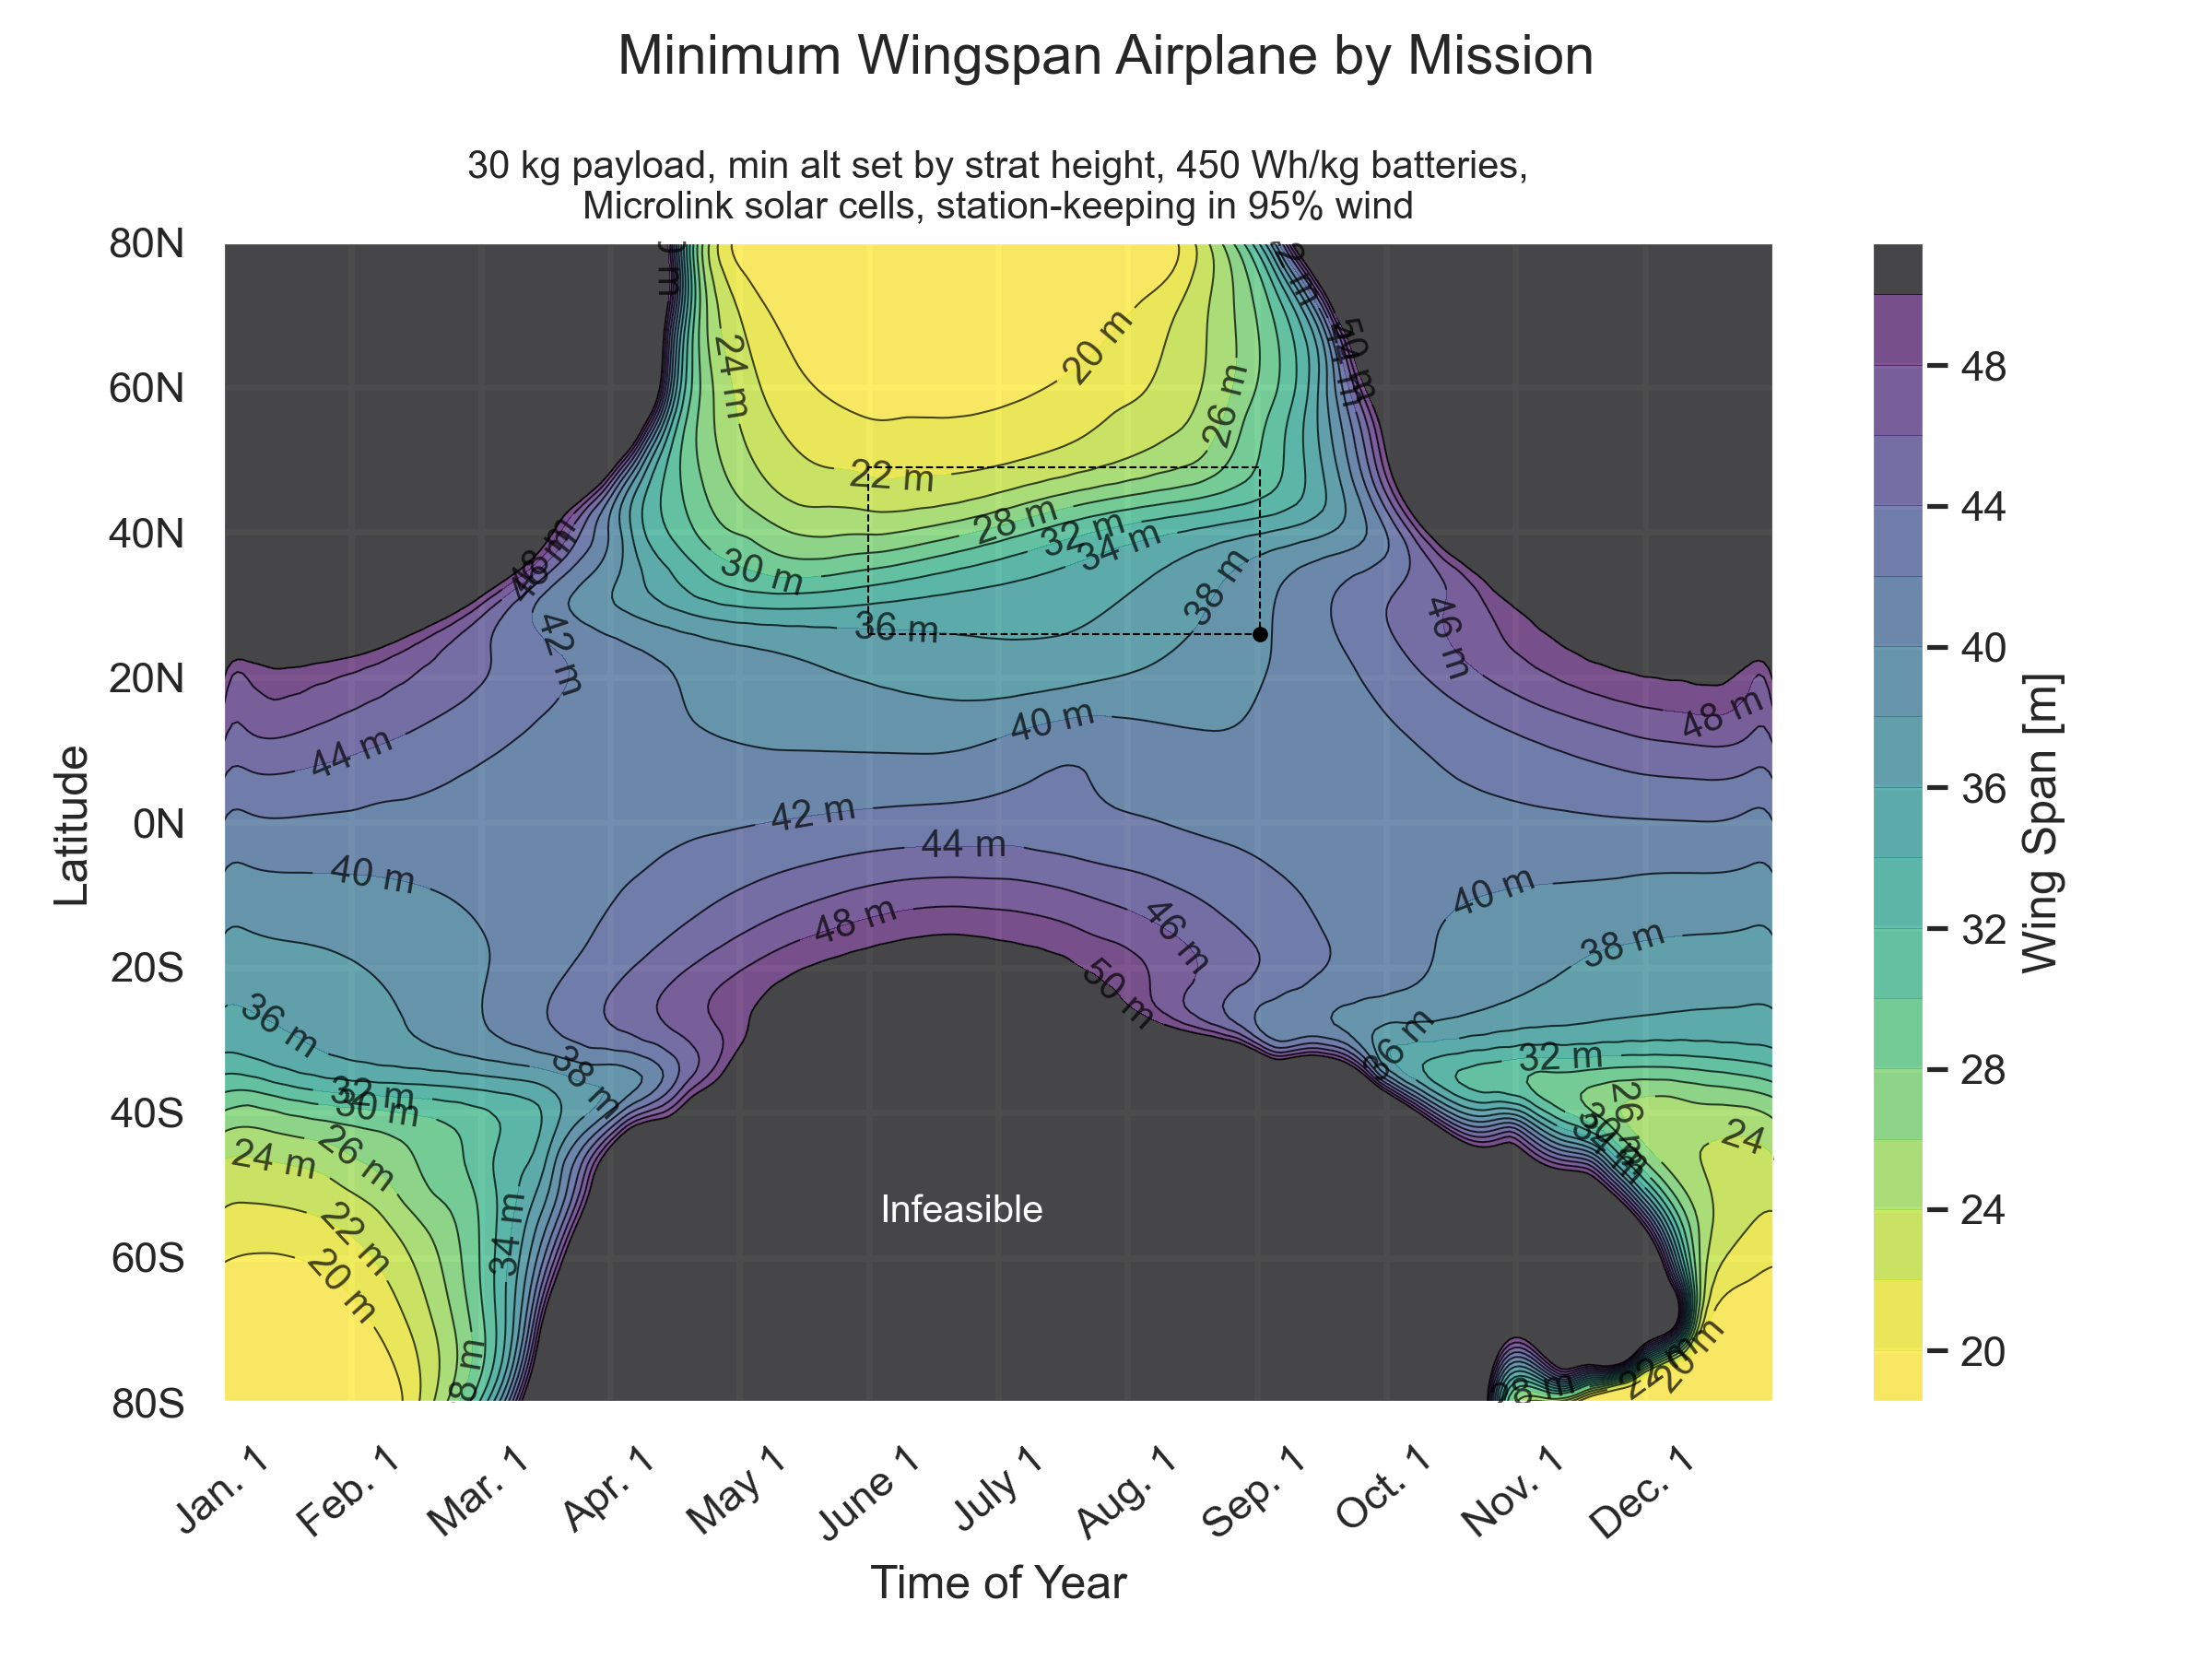
\includegraphics[width=\textwidth]{../figures/dawnfigures/30kg_payloadw_mission.png}
    \caption{Feasibility of a solar aircraft throughout the seasonality-latitude mission space, as measured by the minimum required wingspan of an aircraft that achieves energy closure with the required payload. The baseline science mission, which involves summertime flight over the continental United States, is shown with a dashed black rectangle on the plot. Within this rectangle, the sizing case (i.e., most difficult mission) is shown with a black dot. Reproduced from Sharpe et al. \cite{sharpe_optimization_2021}.}
    \label{fig:dawn_wingspan}
\end{figure}

Early mapping of this broader global mission space allowed the Dawn development team crucial insight into other potential missions of interest, such as Antarctic ice shelf monitoring, wildfire monitoring, methane monitoring, flood monitoring, and others. In a broader sense, this is a useful tool for business development, essentially allowing engineers to ask ``Who else should we be pitching to?'' at the earliest stages of the design process.

\subsubsection*{Rapid Problem Reformulation}

One of the most useful features of a code transformations framework is that the separation between formulation and numerics allows for rapid problem reformulation. For example, suppose that instead of answering the baseline design problem (which assesses wingspan, given some fixed payload), we wish to instead assess what payload would be possible, given some fixed wingspan. This change can be implemented by changing just two lines of code, and after a few minutes of computation, results from this ``flipped problem'' are available for the user. This is shown in Figure \ref{fig:dawn_payload}, where a fixed span of 34 meters is assumed\footnote{Arbitrarily based on the wingspan of the MIT Daedalus aircraft, as a useful point of comparison for the design team.}.

\begin{figure}[h]
    \centering
    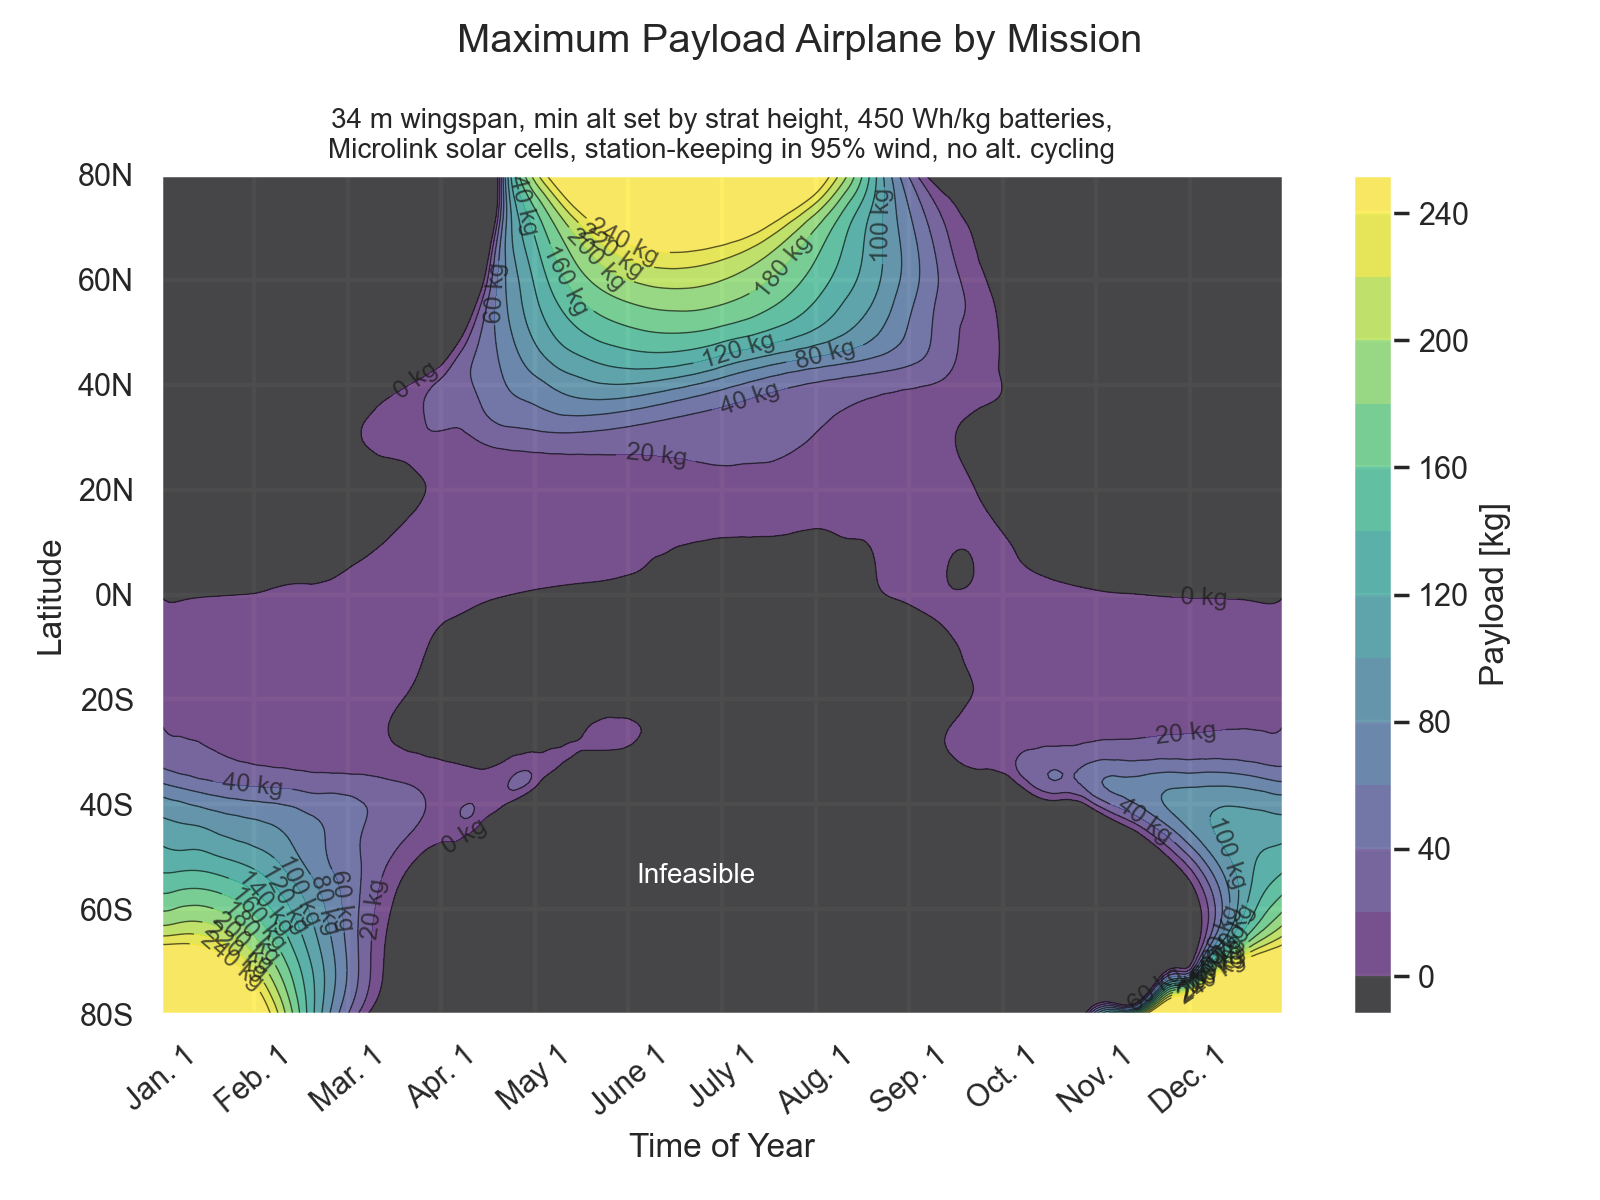
\includegraphics[width=\textwidth]{../figures/dawnfigures/max_payload.png}
    \caption{Feasibility of a solar aircraft throughout the seasonality-latitude mission space, as measured by the maximum payload that can be carried by a clean-sheet aircraft dewign with a fixed wingspan of 34 meters. Equivalent to a ``flipped problem'' of Figure \ref{fig:dawn_wingspan}. Reproduced from Sharpe et al. \cite{sharpe_optimization_2021}.}
    \label{fig:dawn_payload}
\end{figure}

This rapid problem reformulation capability is crucial for the early-stage design process, where the design space is not yet well-understood. By allowing the user to quickly explore the design space in a variety of ways, the design tool can be used to rapidly iterate on the design problem, allowing the user to quickly gain insight into the design space and make informed decisions.

\subsubsection*{Sensitivity Analysis}

Another useful framework-level feature that was developed through the Dawn project was the ability to extract first-order sensitivity information of various constraints and parameters. This information is taken from the dual variables of the optimization problem, which indicates how the performance would change if a single constraint or parameter was modified, while holding all others tight. (This is sometimes called a ``total derivative'' sensitivity.) Because IPOPT is a primal-dual optimizer, these sensitivities can be extracted essentially for free, as they are computed during the optimization process.

Table \ref{tab:dawn_sensitivities} gives a selected subset of these sensitivities for the Dawn design problem. In early design stages, these sensitivities are useful for understanding the design space -- as in the Firefly example of Section \ref{sec:firefly_sweeps}, it is often not the designer's true intent to optimize wholly for one figure of merit at the expense of all others. In later design stages, these sensitivities can (and should) be used to allocate engineering resources. Example such questions could be: a) whether it more valuable to research battery specific energy improvements or drag reductions, or b) whether an alternative motor, which is more efficient but heavier, results in a net performance gain.

\begin{table}[H]
    \centering
    \caption{First-order sensitivities for the point design corresponding to the the baseline mission. Reproduced from Sharpe et al. \cite{sharpe_optimization_2021}}.
    \label{tab:dawn_sensitivities}
    \begin{tblr}{
        colspec={@{} l X X @{}},
        row{1} = {font=\bfseries},
    }
        \toprule
        Figure of Merit                 & Sensitivity of Wingspan & Sensitivity of TOGW \\
        \midrule
        Any added mass                  & 0.22 m/kg               & 4.17 kg/kg          \\
        Any added power draw            & 0.010 m/W               & 0.185 kg/W          \\
        Any added drag                  & 0.479 m/N               & 7.50 kg/N           \\
        Battery spec. energy            & -0.090 m/(Wh/kg)        & -0.960 kg/(Wh/kg)   \\
        Battery packing fraction        & -0.461 m/(\%)           & -4.847 kg/(\%)      \\
        Solar cell efficiency           & -0.464 m/(\%)           & -0.865 kg/(\%)      \\
        Solar cell area density         & 12.4 m/(kg/m$^2$)       & 149 kg/(kg/m$^2$)   \\
        Solar cell usable wing fraction & -10.6 m/(\%)            & 80.9 kg/(\%)        \\
        Propeller efficiency            & -0.613 m/(\%)           & -4.72 kg/(\%)       \\
        Motor efficiency                & -0.586 m/(\%)           & -4.75 kg/(\%)       \\
        Minimum cruise altitude         & 5.10 m/km               & 46.2 kg/km          \\
        \bottomrule
    \end{tblr}
\end{table}

\subsection{Computational Reproducibility}

A publicly-accessible repository of the code used to generate the MIT Dawn conceptual design is available via the \emph{Dawn Design Tool} at \url{https://github.com/peterdsharpe/DawnDesignTool}. We note that this public code has been forked and privately refined in collaboration with the Electra.aero engineering team, so results using this public repository should not be considered representative of any up-to-date design decisions or performance estimates.


\section{Liquid-Hydrogen-Fueled Long-Haul Transport Aircraft}
\label{sec:hydrogen}

A third example aircraft design case study conducted using AeroSandbox was a conceptual design study of a liquid-hydrogen-fueled long-haul transport aircraft.

\subsection{Problem Overview and Background}

At the time of writing, aviation is generally estimated to be responsible for roughly 3\% of anthropogenic climate impacts, with slight variations in this figure depending on method of accounting\footnote{Aviation is roughly 2.5\% of global carbon emissions, but the high-altitude nature of emissions cause disproportionately high impact. Also, non-carbon climate impacts (e.g., contrails, NOx, etc.) may have strong impacts on radiative forcing that are not captured in carbon-focused emissions measures.}. Of this fraction, long-haul aviation (flights with ranges longer than 4,800 km)\footnote{These mostly include intercontinental flights on wide-body aircraft.} contributed roughly 35\% of the total aviation fuel burn \cite{yutko}. This is of particular concern, because while short-haul aviation has more readily-available decarbonization pathways (e.g., electrification), long-haul aviation has very few options to decarbonize due to energy density requirements.

In practice, the two main options for decarbonizing long-haul aviation are synthetic aviation fuels (SAF) and hydrogen-based solutions. While SAF is attractive in the short-term as a potential drop-in solution, the scalability of a SAF-based aviation fuel ecosystem remains an area of concern\footnote{Colloquially, this is often referred to as the ``food vs. fuel'' debate, as the most economically-viable SAF formulations tend to use food feedstock. This drives up food prices and competes for limited arable land. Estimates of the land area required to sustain a global SAF-based aviation economy are similar in scale to the current arable land of the United States.} \cite{waypoint2050, gaubatz_estimating_2023}. Hydrogen, on the other hand, is a more speculative solution, but if scaling SAF proves to be technically, politically, or economically infeasible, it may be the only remaining option for long-haul decarbonization.

Hydrogen is best thought of as a ``carrier'' fuel, similar to a battery, although with much higher energy density. (For comparison, the specific energy of hydrogen is roughly 120 MJ/kg, while kerosene-based fuels give roughly 43 MJ/kg and lithium batteries give roughly 1 MJ/kg.) Because of this, the emissions associated with hydrogen are, of course, highly dependent on the method of hydrogen production. Currently, the most common method of hydrogen production is steam methane reforming (SMR), which is a process that produces hydrogen from natural gas. This process is not carbon-neutral, but it provides an economical on-ramp for a hydrogen economy while electrolysis technologies and grid decarbonization advance\footnote{In the medium term, hydrogen can result in reduced aviation emissions compared to a present-day baseline even without full grid decarbonization. This is especially true if carbon capture utilization and storage (CCUS) is incorporated into the SMR process.} \cite{cascade}. In the long term, ``green hydrogen'' produced by electrolysis powered by low-emissions\footnote{Considering lifecycle emissions} sources (e.g., wind, solar, hydropower, geothermal, nuclear) could dramatically reduce the carbon impact of long-haul aviation.

Hydrogen may be stored in either a high-pressure gaseous (\gh) or a cryogenic liquid (\lh) form, each of which come with their own unique challenges. For long-haul aviation, \lh is universally preferred due to its much higher effective specific energy (i.e., specific energy with the tank mass included). For example, with \lh, the tank gravimetric efficiency $\eta_{\rm tank}$ (essentially, the mass fraction of a filled tank that is hydrogen) is usually 50--75\% \cite{brewer_hydrogen_1991}; for \gh, this is typically 8--12\%. The higher volumetric density of \lh relative to \gh also allows for more compact tank designs, which reduces the drag impact at the aircraft level.

In addition to the grid decarbonization and hydrogen production challenges, hydrogen presents a number of unique operational difficulties at the aircraft-level. Interestingly, the common concern of crash safety is not actually a major one (relative to kerosene-based fuels), as a) in the event of a post-crash fire, hydrogen is a buoyant gas at STP, which directs heat upwards and prevents on-ground fuel pooling; and b) hydrogen burns with minimal soot\footnote{In post-crash fires on kerosene-fueled aircraft, smoke inhalation often causes the majority of injuries.}. In-flight fire is also a risk that can be mitigated to acceptable levels, through a combination of positive-pressure tanks, gas sniffers, and boiloff vents \cite{brewer_hydrogen_1991}. However, safe hydrogen refueling is challenging and several important open research questions remain \cite{gaubatz_estimating_2023}. For example, fuel lines must be purged for safety every time the aircraft is refueled, and a cryogenic fuel presents significant limitations on how this can be done\footnote{For example, common purge gases like nitrogen and argon will freeze at \lh temperatures; other gases, like helium, must be used.}.

Aircraft performance is also a significant concern when hydrogen is introduced. For example, both \lh and \gh tanks benefit from a low-surface-area-to-volume ratio, which makes traditional storage within wings impractical. Instead, hydrogen is typically stored in cylindrical or conformal fuselage tanks. Relative to traditional wing storage, this a) loses the benefit of spanloading, leading to increased structural weight in the wing and fuselage, b) can create a significant center-of-gravity shift during fuel burn, depending on configuration, and c) usually yields a (small) aerodynamic penalty due to the increased volume of the fuselage. In addition, tank weight is much higher\footnote{In the case of \gh, this is due to pressurization stress, and in the case of \lh, this is due to insulation and boil-off considerations.}, fuel lines are heavier, and fuel pumping becomes much more complex\footnote{For example, rotating components in a pump usually cannot be lubricated, because these oils freeze well above the boiling point of \lh. Hydrogen embrittlement also limits pump life.}. Brewer gives one of the most thorough overviews of these opportunities and challenges \cite{brewer_hydrogen_1991}.

On the other hand, the much higher specific energy of hydrogen compared to kerosene results in far smaller required fuel mass fractions\footnote{For example, even after accounting for increased tank weight, \lh offers a \emph{realizable} specific energy that is roughly double that of kerosene-based fuels.}. Because of this, it is not obvious whether the net aircraft performance impact of hydrogen is positive or negative relative to existing kerosene-based aircraft, and studies find results that vary strongly based on assumptions \cite{cascade, gaubatz_estimating_2023, tiwari_review_2024}.

In short, the motivation for exploring hydrogen as an aviation fuel is not that it is particularly attractive or easy to work with; instead, it is because a genuine possibility exists that it may be the \emph{only} scalable solution for long-haul aviation decarbonization. Hydrogen converts a problem that may otherwise be impossible to solve (decarbonizing long-haul aviation) into a problem that, while still challenging, is at least technically solvable (decarbonizing the electricity grid).

\subsection{Aircraft Design Problem Formulation}

In this study, we formulated an aircraft design problem for a hydrogen-fueled long-haul transport aircraft, with the goal of learning more about aircraft performance deltas from kerosene designs. The key design requirements were modeled after specifications of a Boeing 777-300ER, which is a representative modern kerosene-fueled long-haul aircraft. These requirements are given in Table \ref{tab:h2_requirements}. In addition, this study assumes that a clean-sheet airplane and engines are used, and that such engines are designed around a 2023 technology level (roughly comparable to a GE9X engine).

\begin{table}[H]
    \centering
    \caption{Key design requirements for the \lh-fueled long-haul transport aircraft design.}
    \label{tab:h2_requirements}
    \begin{tblr}{
        colspec={@{} X X X @{}},
        row{1} = {font=\bfseries},
    }
        \toprule
        Specification                 & Value             & Motivation                                 \\
        \midrule
        \# of Passengers              & 400               & Long-haul demand                           \\
        Ultimate Range (fully loaded) & > 7,500 nmi       & Long-haul demand                           \\
        Cruise Mach                   & > 0.75            & 2x / day turnaround, market acceptance     \\
        Wing Span                     & < 64.8 m (213 ft) & FAA AC 150/5300-13 ICAO Group V: 52 – 65 m \\
        Engine-out Climb Gradient     & > 2.4\%           & Part 25.121                                \\
        Fuel Source                   & Hydrogen          &                                            \\
    \end{tblr}
\end{table}

A three key configuration-level decisions were made a priori based on existing literature:
\begin{enumerate}
    \item Choice of \lh fuel, rather than \gh, due to its significantly higher realizable specific energy.
    \item Choice to place fuel in two conformal forward and aft tanks in the fuselage, which results in a smaller center-of-gravity shift during fuel burn compared to a single aft tank\footnote{Having one aft tank requires a larger horizontal stabilizer in order to trim during the center of gravity shift, costing drag. Also, multiple tanks are needed anyway for FAR 25 certification under current guidance.}. Other tank configurations were considered and not selected for boil-off reasons.
    \item Choice to use direct hydrogen combustion, rather than fuel cells, due to much higher specific power.
\end{enumerate}

More details on the motivations for these decisions, and possible alternative ones, are given in the author's contributions to prior work by Gaubatz et al. \cite{gaubatz_estimating_2023}.

From this set of requirements a vehicle design optimization problem was formulated, using the problem setup shown in Figure \ref{fig:h2_formulation}. Unlike the Firefly and Dawn problems, this problem was formulated as a single-point design problem, rather than a trajectory optimization problem. This is because the vehicle performance is dominated by cruise performance, and during this phase it is assumed to operate at a constant design lift coefficient and Mach number. (This implies that a step climb is performed throughout cruise as fuel is burned and mass decreases, which is common in practice and described further by Drela in material related to the TASOPT code \cite{drela_tasopt_2010}.) Using Breguet-range-like relations, the aircraft's total fuel burn can be computed from this representative optimized cruise operating point.

In the formulation of Figure \ref{fig:h2_formulation}, the objective function the \emph{transport energy efficiency}, which is defined as the chemical potential energy of the fuel burned divided by the economically-useful work (measured in passenger-miles) performed by the aircraft. This metric, which is common in green transportation studies, is often used to compare economic viability across both renewable and nonrenewable solutions, which are otherwise difficult to compare directly \cite{waypoint2050}.

\begin{figure}[h]
    \centering
    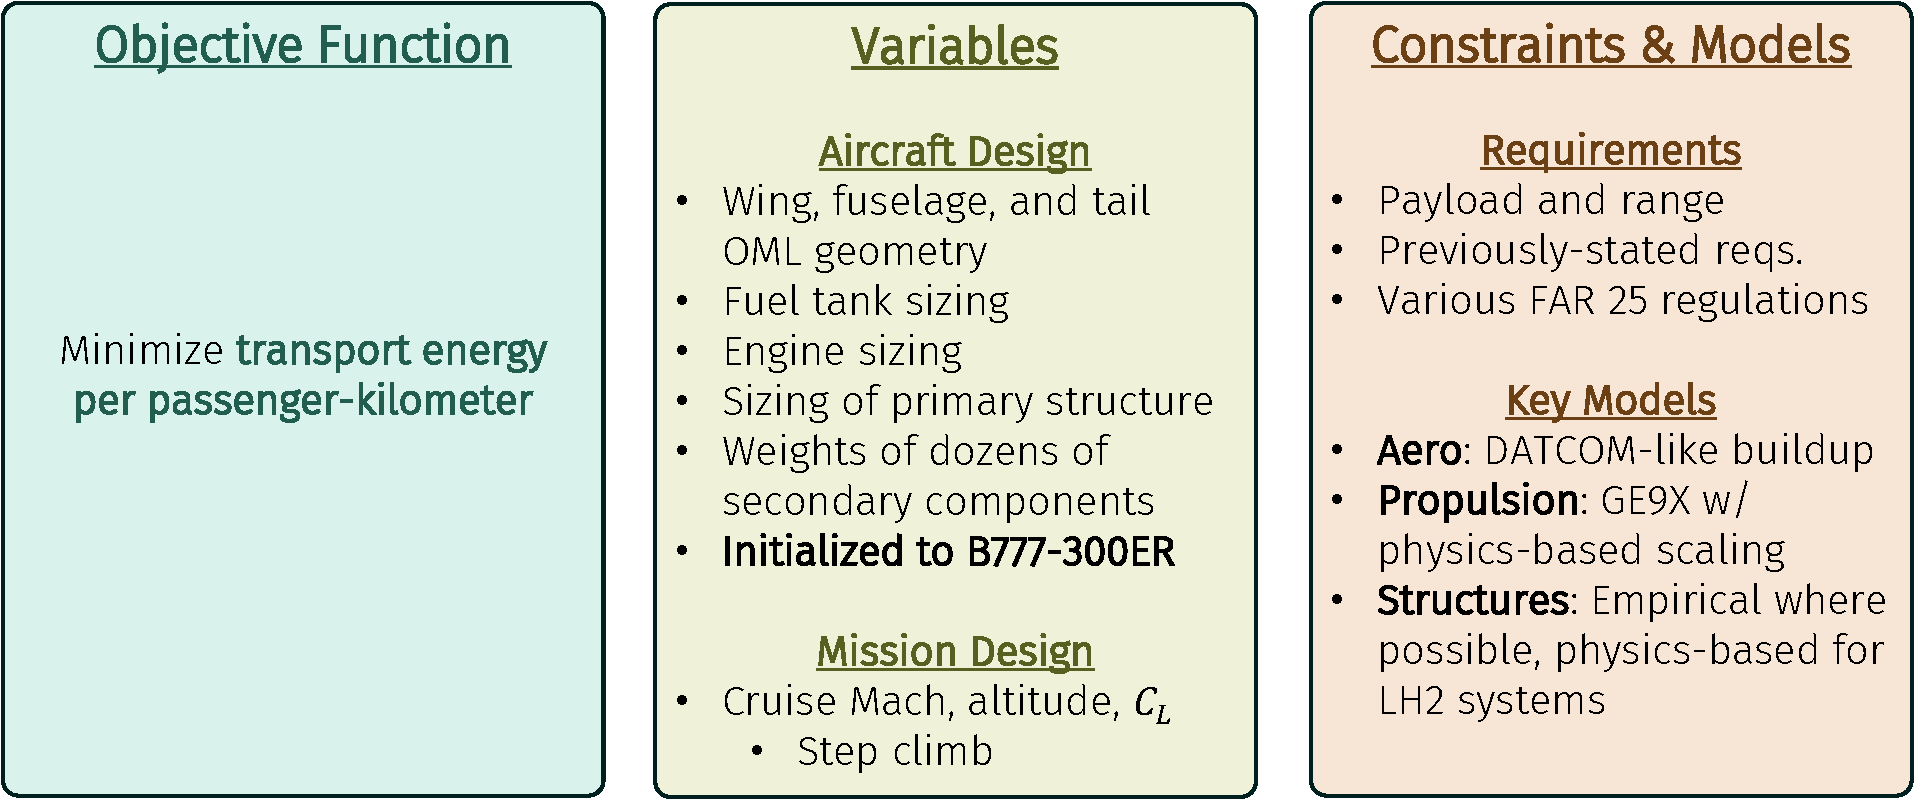
\includegraphics[width=\textwidth,page=1]{../figures/Hydrogen_figures-crop.pdf}
    \caption{High-level design optimization problem formulation for a liquid-hydrogen-fueled long-haul transport aircraft.}
    \label{fig:h2_formulation}
\end{figure}

\subsection{Results}

This problem is formulated and solved using AeroSandbox, yielding a point design for a \lh-fueled transport aircraft. Using the AeroSandbox aircraft geometry stack, a three-view design can be generated and presented to the user, which has been further illustrated to yield Figure \ref{fig:h2_three_view}. Overall, the resulting configuration is similar to a Boeing 777-300ER, with a few notable changes: a clean-sheet airframe and engines, much higher realizable fuel specific energy, and a wider cabin that accommodates a 4-5-4 seating arrangement. In Figure \ref{fig:h2_three_view}, this substantial increase in fuselage width somewhat visually obscures the large volume occupied by the conformal hydrogen tanks.

Another immediate change that is apparent in Figure \ref{fig:h2_three_view} is the placement of the flight deck, which has no forward visibility. This solves pressurization and access challenges, but requires a camera-based forward visibility system. Existing certification pathways of enhanced flight vision systems (EFVS) and synthetic vision systems (SVS) may be used to certify this IFR-only flight deck configuration, but this is an open research question.

\begin{figure}[h]
    \centering
    \includesvg[width=\textwidth]{../figures/Hydrogen/ppt/media/image25.svg}
    \caption{Three-view drawing of the \lh-fueled long-haul transport aircraft design.}
    \label{fig:h2_three_view}
\end{figure}

The results of the AeroSandbox optimization study can also be quantitatively shown in Table \ref{tab:h2_results}. In this table, the key performance metrics of the \lh-fueled aircraft are compared to those of an equivalent kerosene-fueled aircraft, which was optimized using an identical methodology and assumptions. This is useful to isolate the impact of fuel choice on various performance parameters. In addition, the as-built Boeing 777-300ER is shown in the table for comparison, which allows the overall accuracy of the optimization model to be assessed. The higher gross weight of the B777 aircraft is partially explained by its higher ultimate range than the optimized aircraft in this study.

\begin{table}[H]
    \centering
    \caption{Key results of the \lh-fueled long-haul transport aircraft design. Comparisons are made to a kerosene-fueled aircraft optimized using an identical methodology and assumptions, as well as to an as-built Boeing 777-300ER.}
    \label{tab:h2_results}
    \begin{tblr}{
        colspec={@{} l X X X @{}},
        row{1} = {font=\bfseries},
        row{13} = {font=\bfseries},
        column{3-4} = {fg=black!70},
    }
        \toprule
        & Optimized \lh Airplane & Optimized Kerosene Airplane & As-Built B777-300ER \cite{b777} \\
        \midrule
        \# of passengers & 400                    & 400                         & 396                             \\
        Ultimate range   & 7,500 nmi              & 7,500 nmi                   & 8,200 nmi (estimated)           \\
        Cruise Mach      & 0.82                   & 0.83                        & 0.84                            \\
        Cruise Altitude  & 36,800 ft              & 36,900 ft                   & 43,100 ft                       \\
        Gross Weight     & 267,800 kg             & 300,800 kg                  & 351,500 kg                      \\
        Empty Weight     & 184,700 kg             & 150,200 kg                  & 167,800 kg                      \\
        Fuel Capacity    & 44,100 kg              & 111,600 kg                  & 145,500 kg                      \\
        Wing Span        & 64.8 m                 & 64.8 m                      & 64.8 m                          \\
        Length           & 81.5 m                 & 73.0 m                      & 73.9 m                          \\
        Lift/Drag        & 15.5                   & 16.6                        & -                               \\
        Fuel Burn        & 7.94 g/pax-km          & 20.1 g/pax-km               & 19.4 to 26.1 g/pax-km           \\
        Transport Energy & 0.95 MJ/pax-km         & 0.86 MJ/pax-km              & 0.84 to 1.13 MJ/pax-km          \\
        \bottomrule
    \end{tblr}
\end{table}

Notably, Table \ref{tab:h2_results} indicates that the transport energy efficiency of the \lh-fueled aircraft is slightly worse than that of the kerosene-fueled aircraft. Most of this can be attributed to the higher empty weight of the \lh aircraft, which cannot take advantage of the spanloading ability of kerosene-fueled aircraft. This leads to higher structural weight in the wing and fuselage.

For a more detailed breakdown of the mass changes as a result of fuel choice, we can inspect the mass budgets of the \lh and kerosene aircraft designs directly. Recent versions of AeroSandbox support mass properties data structures that allow visualizations of these budgets to be generated automatically. Figures \ref{fig:h2_mass_budget} and \ref{fig:kerosene_mass_budget} show the mass budgets of the \lh and kerosene aircraft designs, respectively. These figures show that the \lh aircraft has a much lower fuel mass fraction than the kerosene aircraft; however, it is offset by increased weight in the wing, fuselage, and fuel tanks.

\begin{figure}[h]
    \centering
%    \includegraphics[width=0.5in,page=2, trim={2in 0 2in 0}]{../figures/Hydrogen_figures-crop.pdf}
    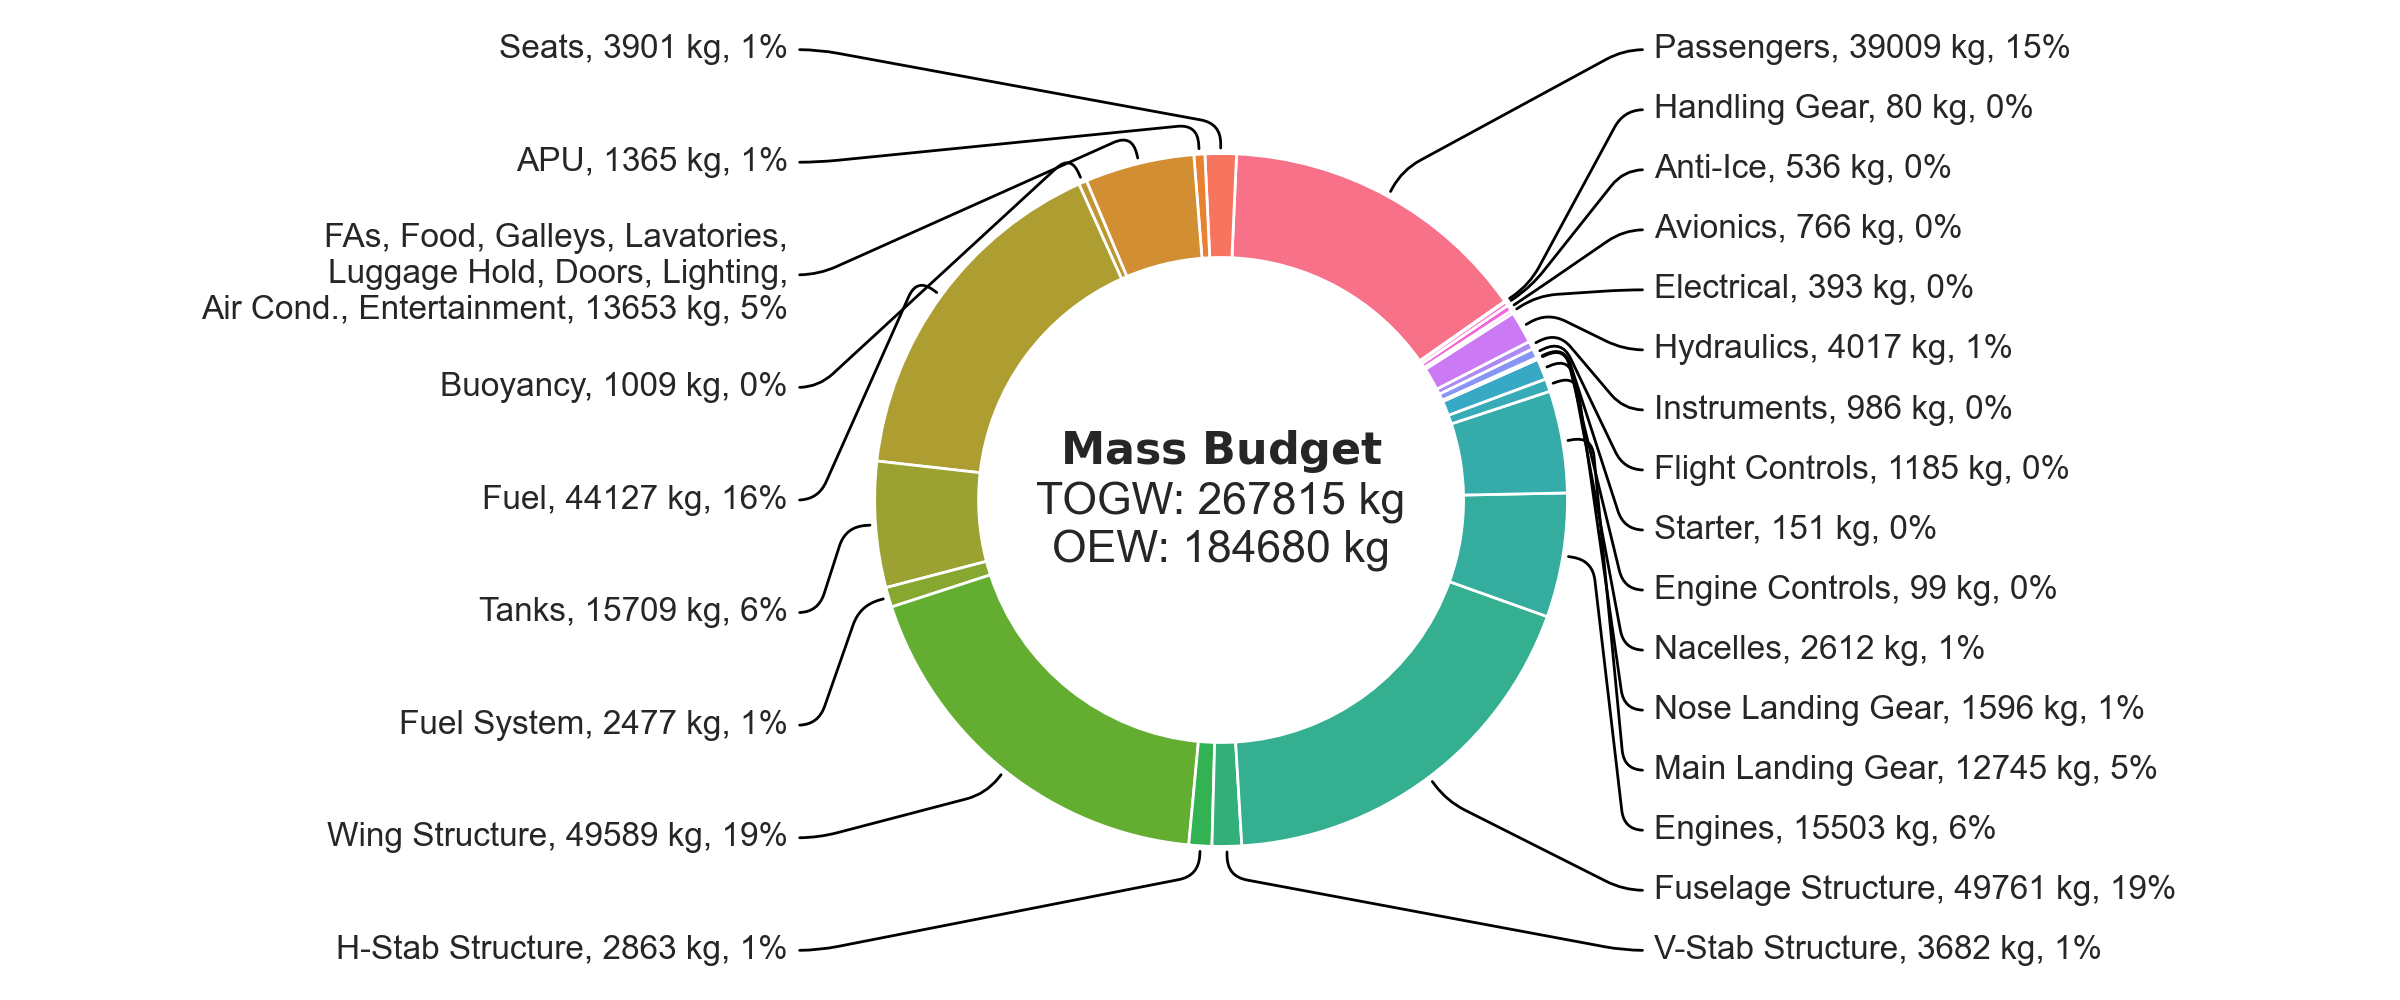
\includegraphics[width=\textwidth, trim={3in 0 3in 0}]{../figures/Hydrogen/ppt/media/image27.png}
    \caption{Mass budget for the \textbf{\lh}-fueled aircraft design. Takeoff gross weight (TOGW) and operating empty weight (OEW) are given in the center of the diagram.}
    \label{fig:h2_mass_budget}
\end{figure}

\begin{figure}[h]
    \centering
    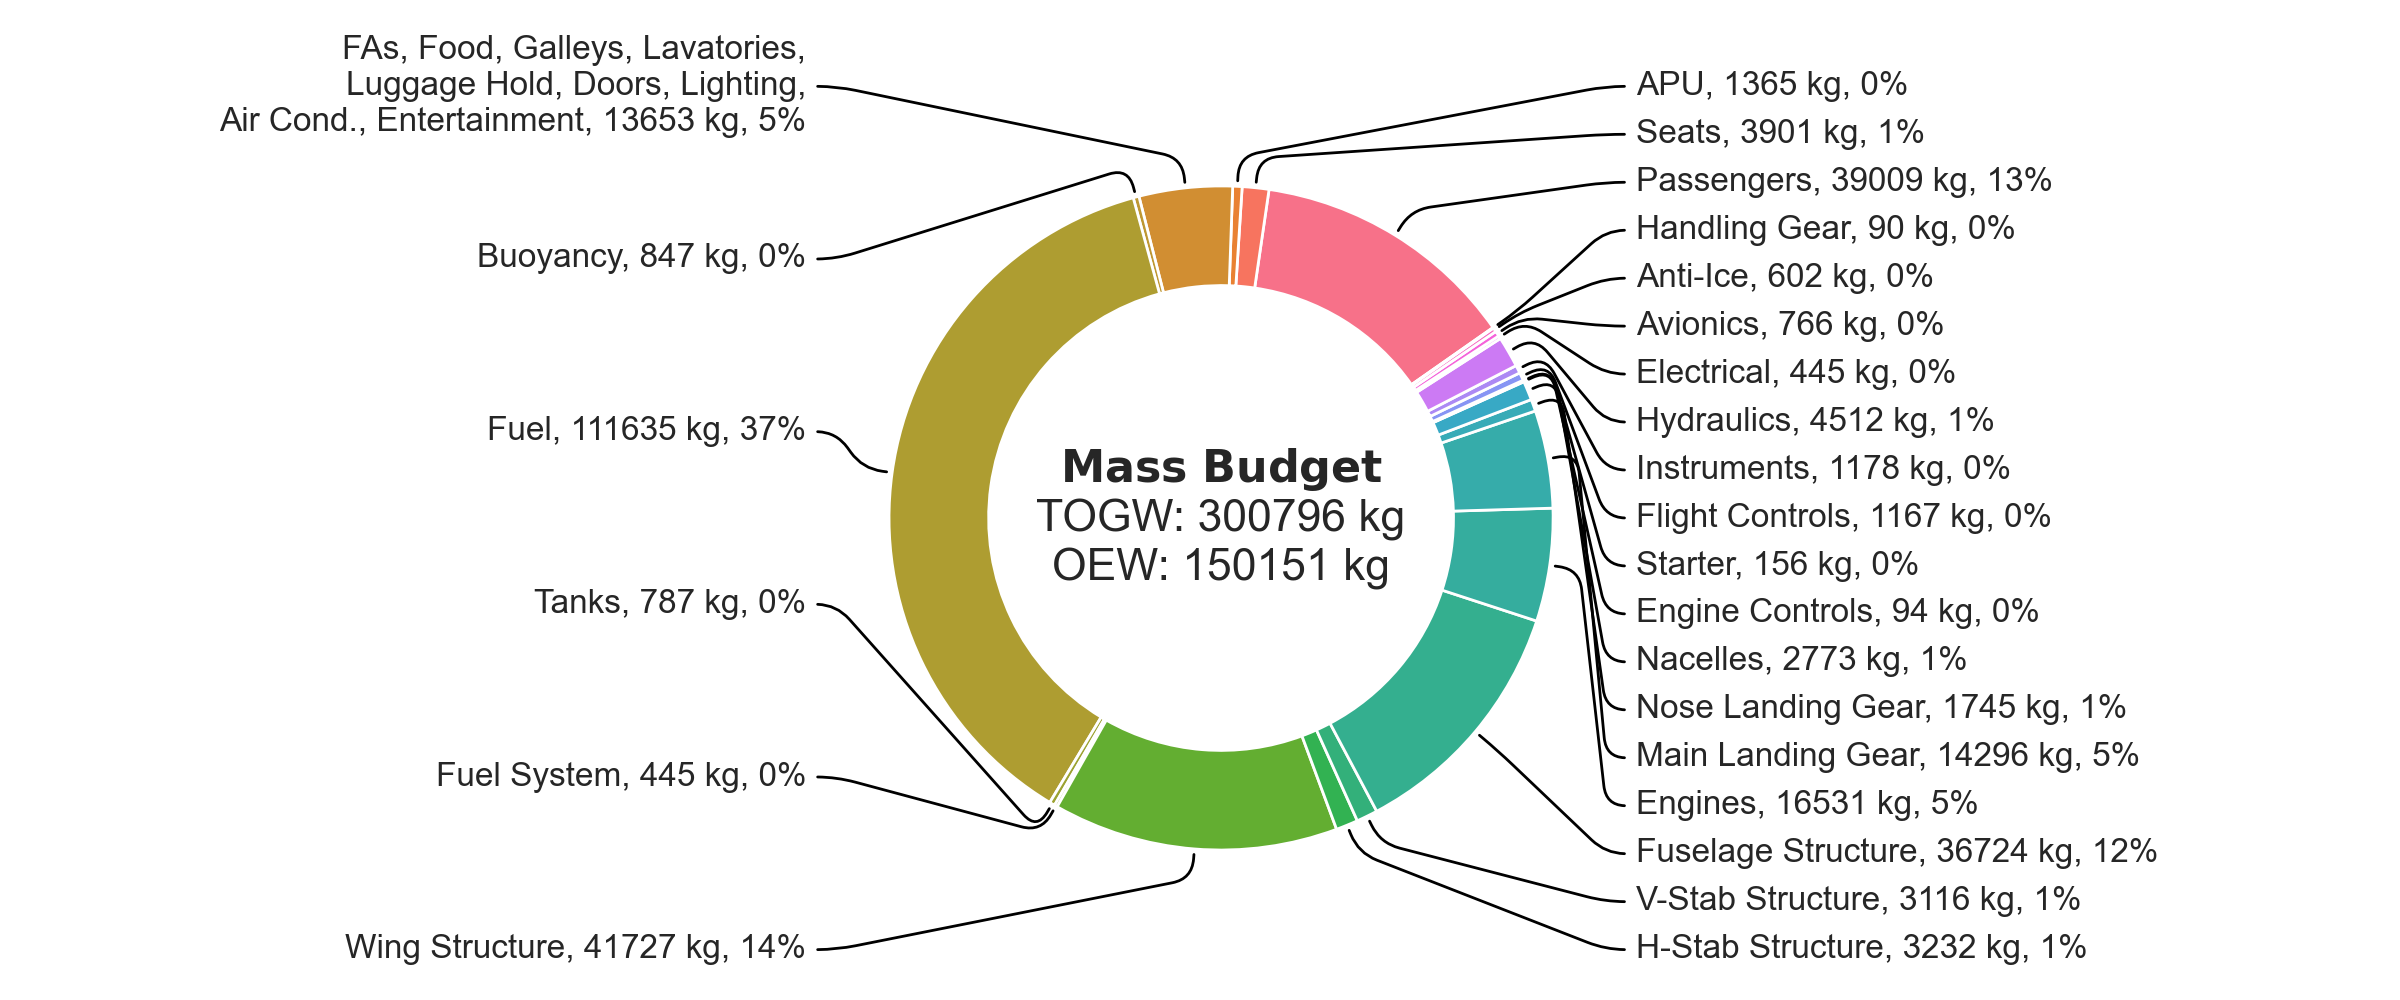
\includegraphics[width=\textwidth, trim={3in 0 3in 0}]{../figures/Hydrogen/ppt/media/image26.png}
    \caption{Mass budget for an equivalent \textbf{kerosene}-fueled aircraft design. Takeoff gross weight (TOGW) and operating empty weight (OEW) are given in the center of the diagram.}
    \label{fig:kerosene_mass_budget}
\end{figure}

\subsection{Performance Sweeps}

As with the Firefly example, exploring the impact of a given technology assumption on the design is as simple as changing two lines of code within a procedural-style code transformations framework. Here, the impact of the tank gravimetric efficiency $\eta_{\rm tank}$ on the transport energy efficiency of the \lh-fueled aircraft design was explored. The results of this study are shown in Figure \ref{fig:transport_energy}, which shows that the relative performance of the \lh-fueled aircraft design is highly sensitive to the tank gravimetric efficiency. Given that current tanks have $\eta_{\rm tank}$ values between 50--75\% \cite{brewer_hydrogen_1991}, this implies that \lh transport aircraft are roughly competitive with kerosene-fueled aircraft in terms of transport energy efficiency. This chart also demonstrates why \gh-based aircraft (with $\$\eta_{\rm tank} \approx 10\%$) are wholly infeasible for long-haul aircraft. Finally, this chart gives a clear explanation as to why the relative transport energy of hydrogen aircraft varies so widely in the aircraft design literature -- it is highly sensitive to the assumed tank technology.

\begin{figure}[h]
    \centering
    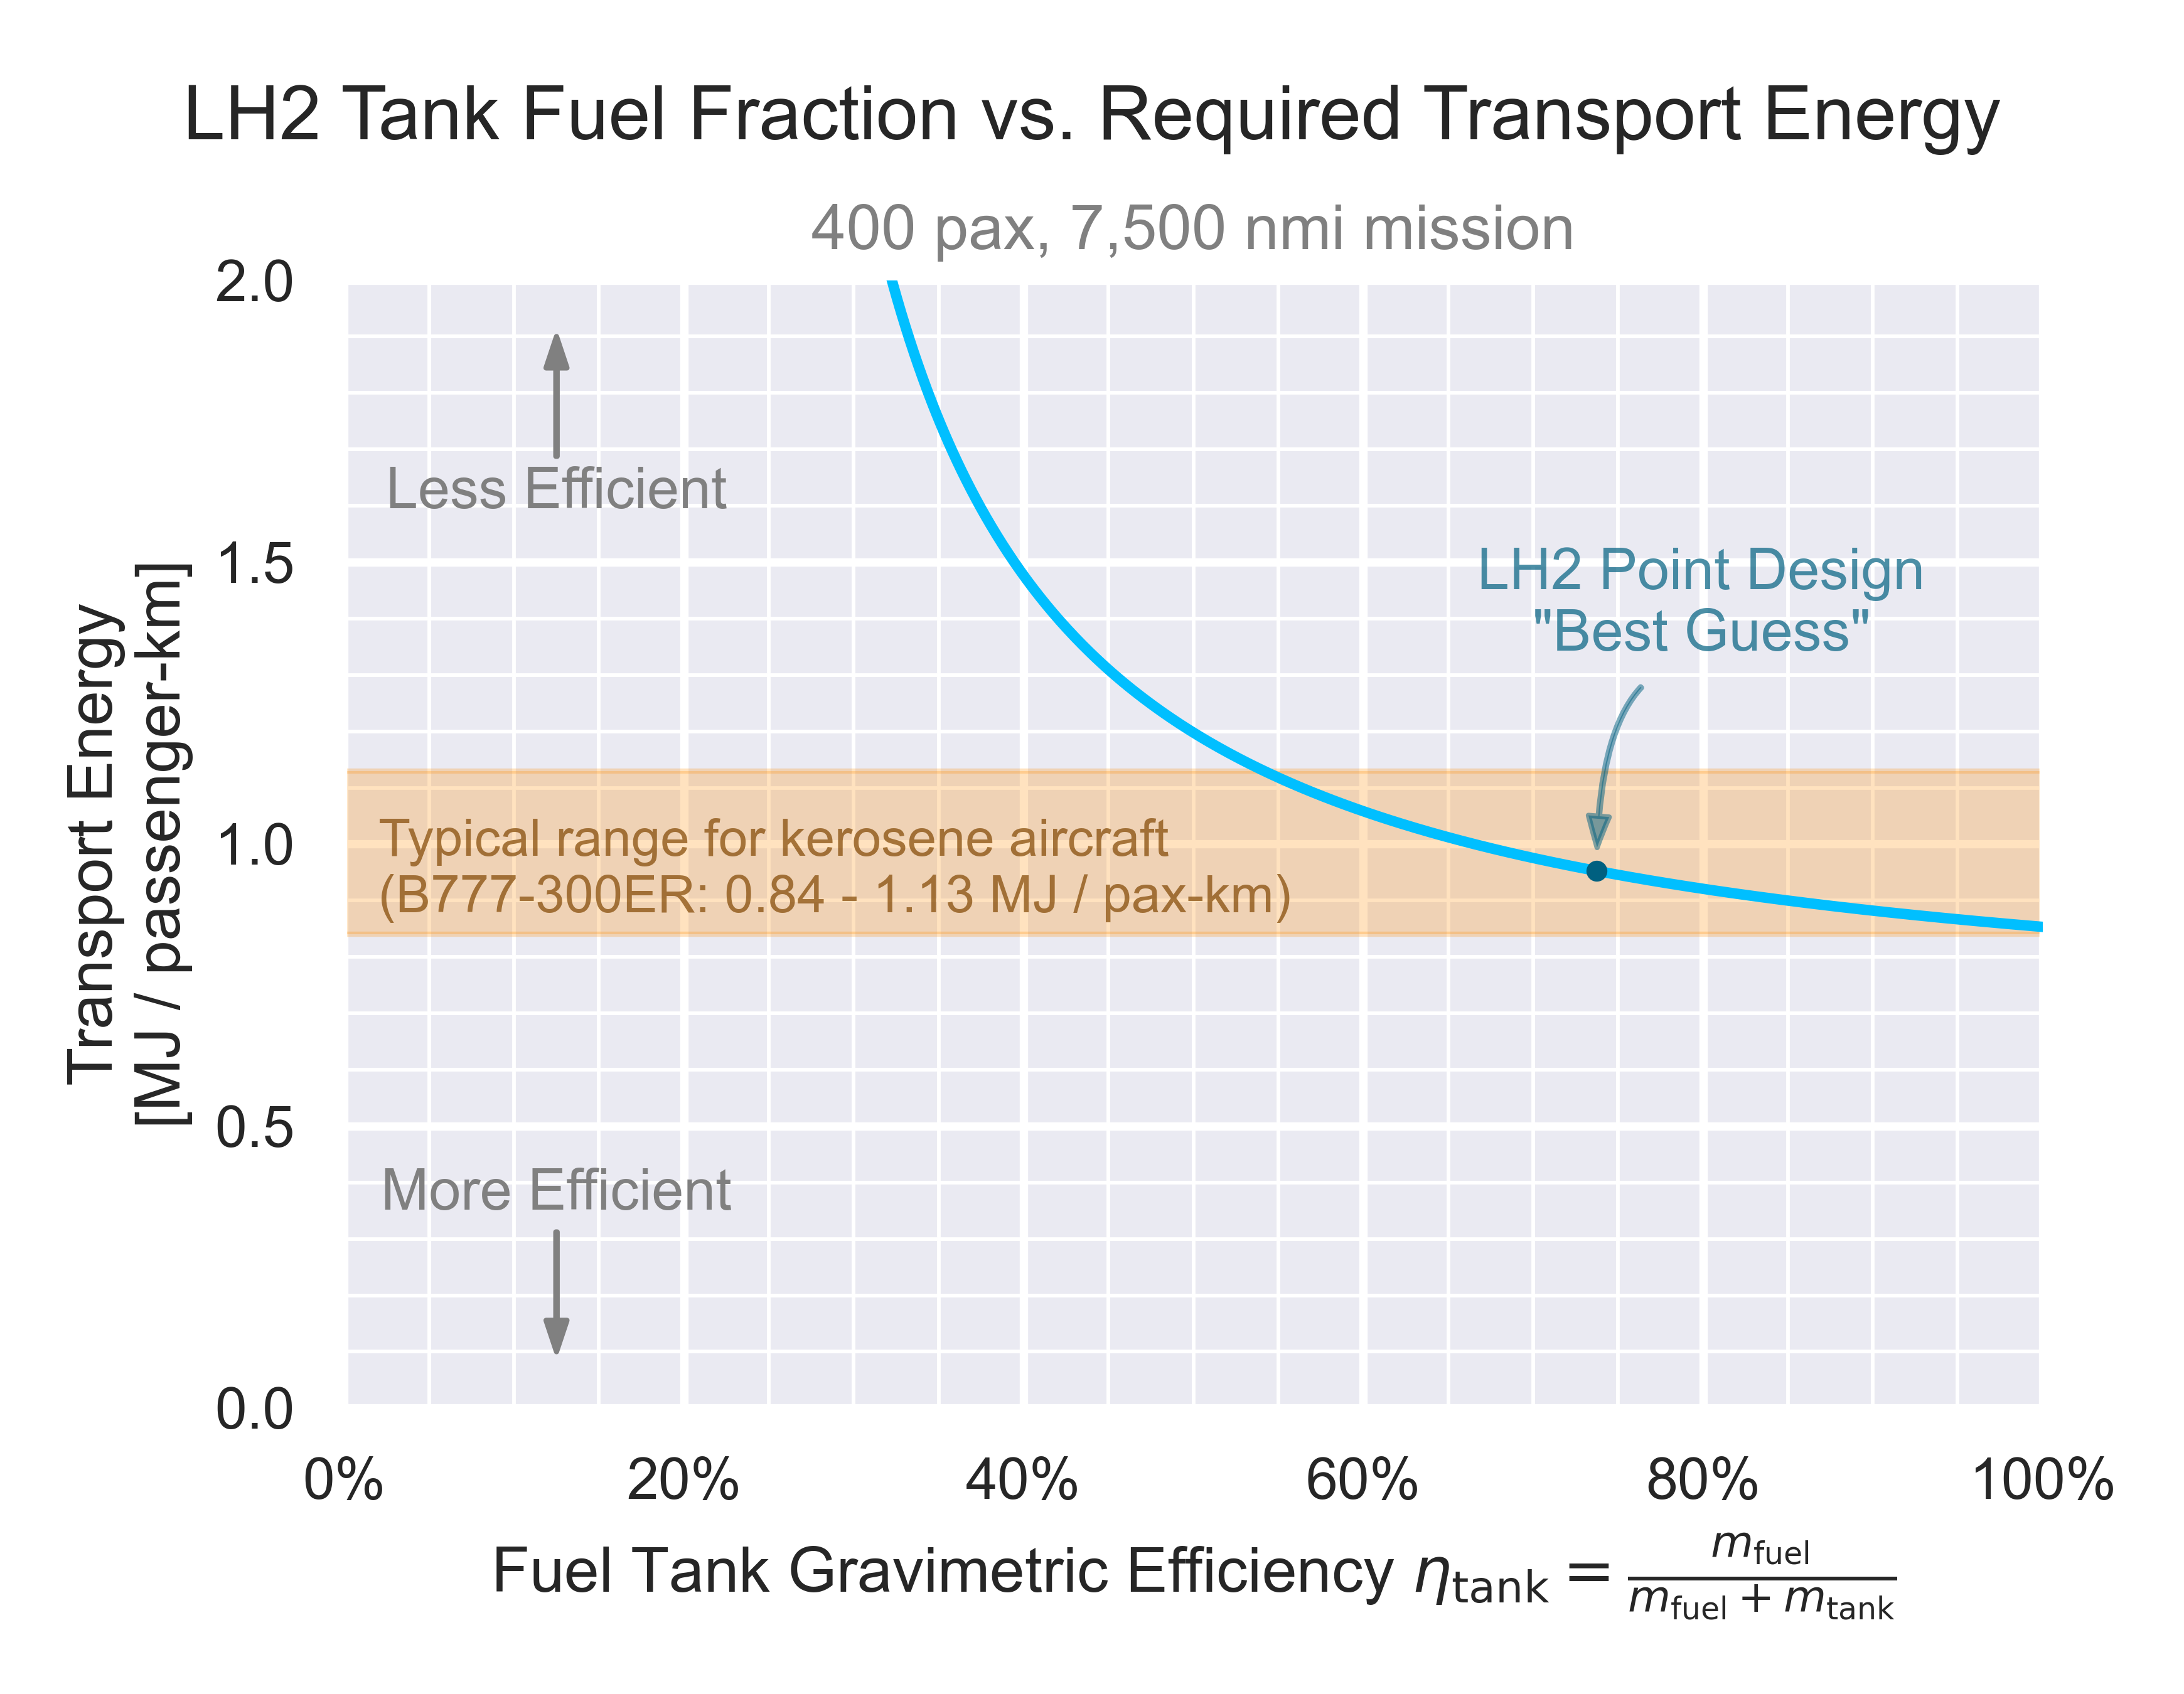
\includegraphics[width=\textwidth]{../figures/Hydrogen/ppt/media/image28.png}
    \caption{Comparison of transport energy efficiency of \lh- and kerosene-fueled aircraft, designed around the same mission. Relative performance depends strongly on the \lh tank gravimetric efficiency, which forms a critical performance metric.}
    \label{fig:transport_energy}
\end{figure}

\subsection{Fleet Design and Market Considerations}

Another example of how a rapid design tool can be used is to explore business-level impacts of a technology choice. To explore just the tip of the iceberg here, here we show how one might think about covering a market of many long-haul flights with different ranges.

First, consider the payload-range diagram of the \lh-fueled aircraft design, shown in Figure \ref{fig:h2_payload_range}. This diagram shows the maximum payload that can be carried by the aircraft as a function of range, a key metric of usefulness for an airline. For example, in this simplified model, the aircraft can carry 400 passengers at its design range of 7,500 nmi. For flights slightly longer than this range, the aircraft must reduce the fuel burn by carrying fewer passengers. For flights shorter than this range, the aircraft is seat-limited to its 400 passenger capacity; however, what is not shown here is that less fuel can be carried, which reduces the aircraft's fuel burn and improves its transport energy efficiency.

\begin{figure}[h]
    \centering
    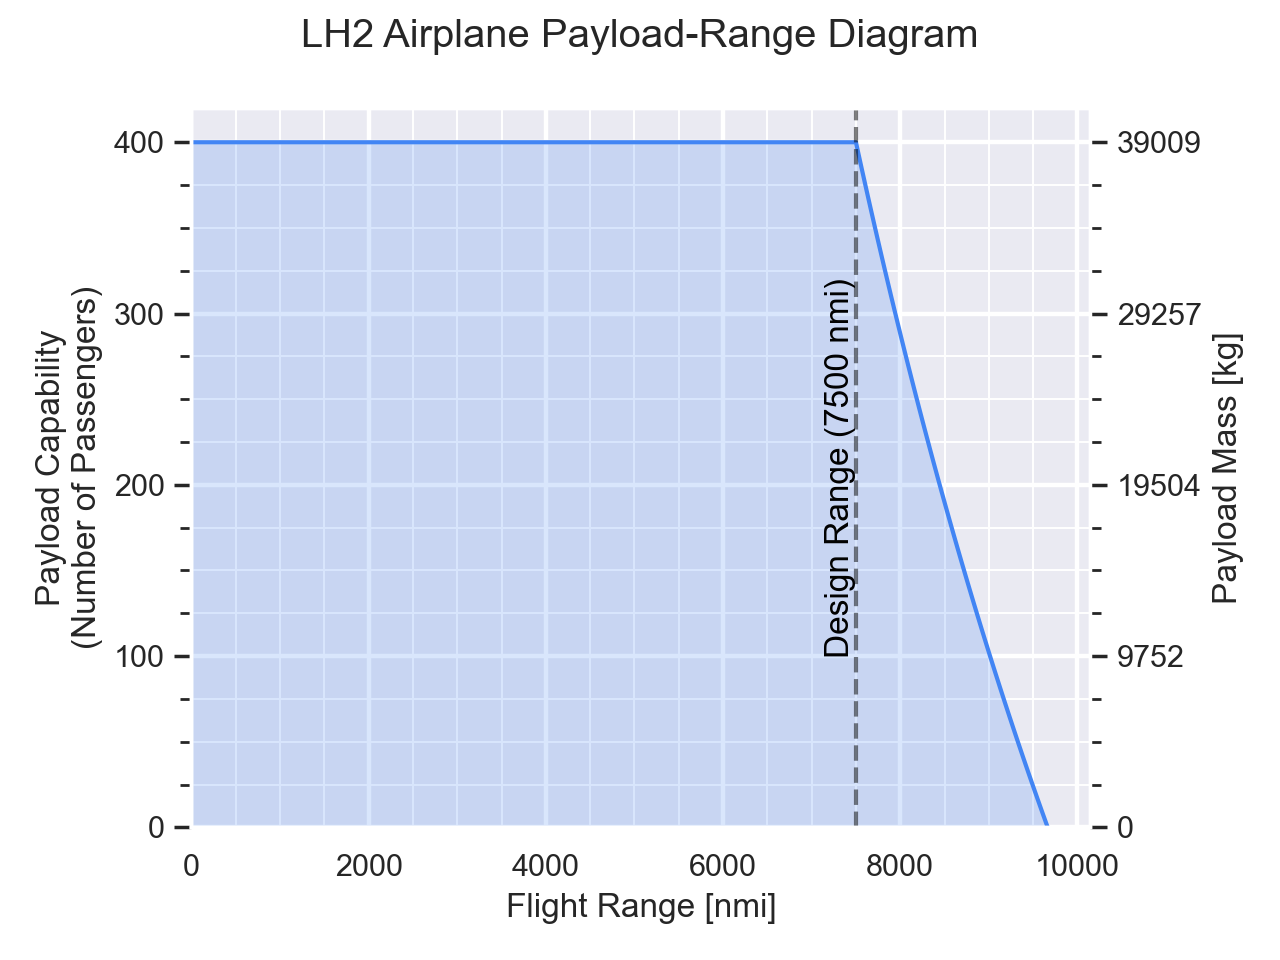
\includegraphics[width=5in]{../figures/Hydrogen/ppt/media/image30.png}
    \caption{Payload-range diagram for the \lh-fueled aircraft design.}
    \label{fig:h2_payload_range}
\end{figure}

However, this improvement in transport energy efficiency for shorter-than-maximum-range flights is not the same for \lh- and kerosene-fueled aircraft. This is because the fuel mass fraction of the \lh aircraft is much lower than that of the kerosene aircraft, so a hydrogen aircraft achieves less benefit from flying shorter-range flights. This is illustrated in Figure \ref{fig:market_segmentation}, where each line shows the transport energy of a particular optimized aircraft design as a function of range. (For each aircraft, the design range is indicated by a dot on the line.) As an operator, the effective transport efficiency \emph{of the combined fleet} is the lower-bound envelope of these curves. Notably, for a kerosene aircraft, there is a relatively small benefit to flying the ``right size airplane for a given mission'', so the market can be covered with two aircraft without much loss in efficiency. For a hydrogen aircraft, this is not the case, and the market must be segmented more finely to achieve the same efficiency.

\begin{figure}[h]
    \centering
    \begin{subfigure}[b]{0.49\textwidth}
        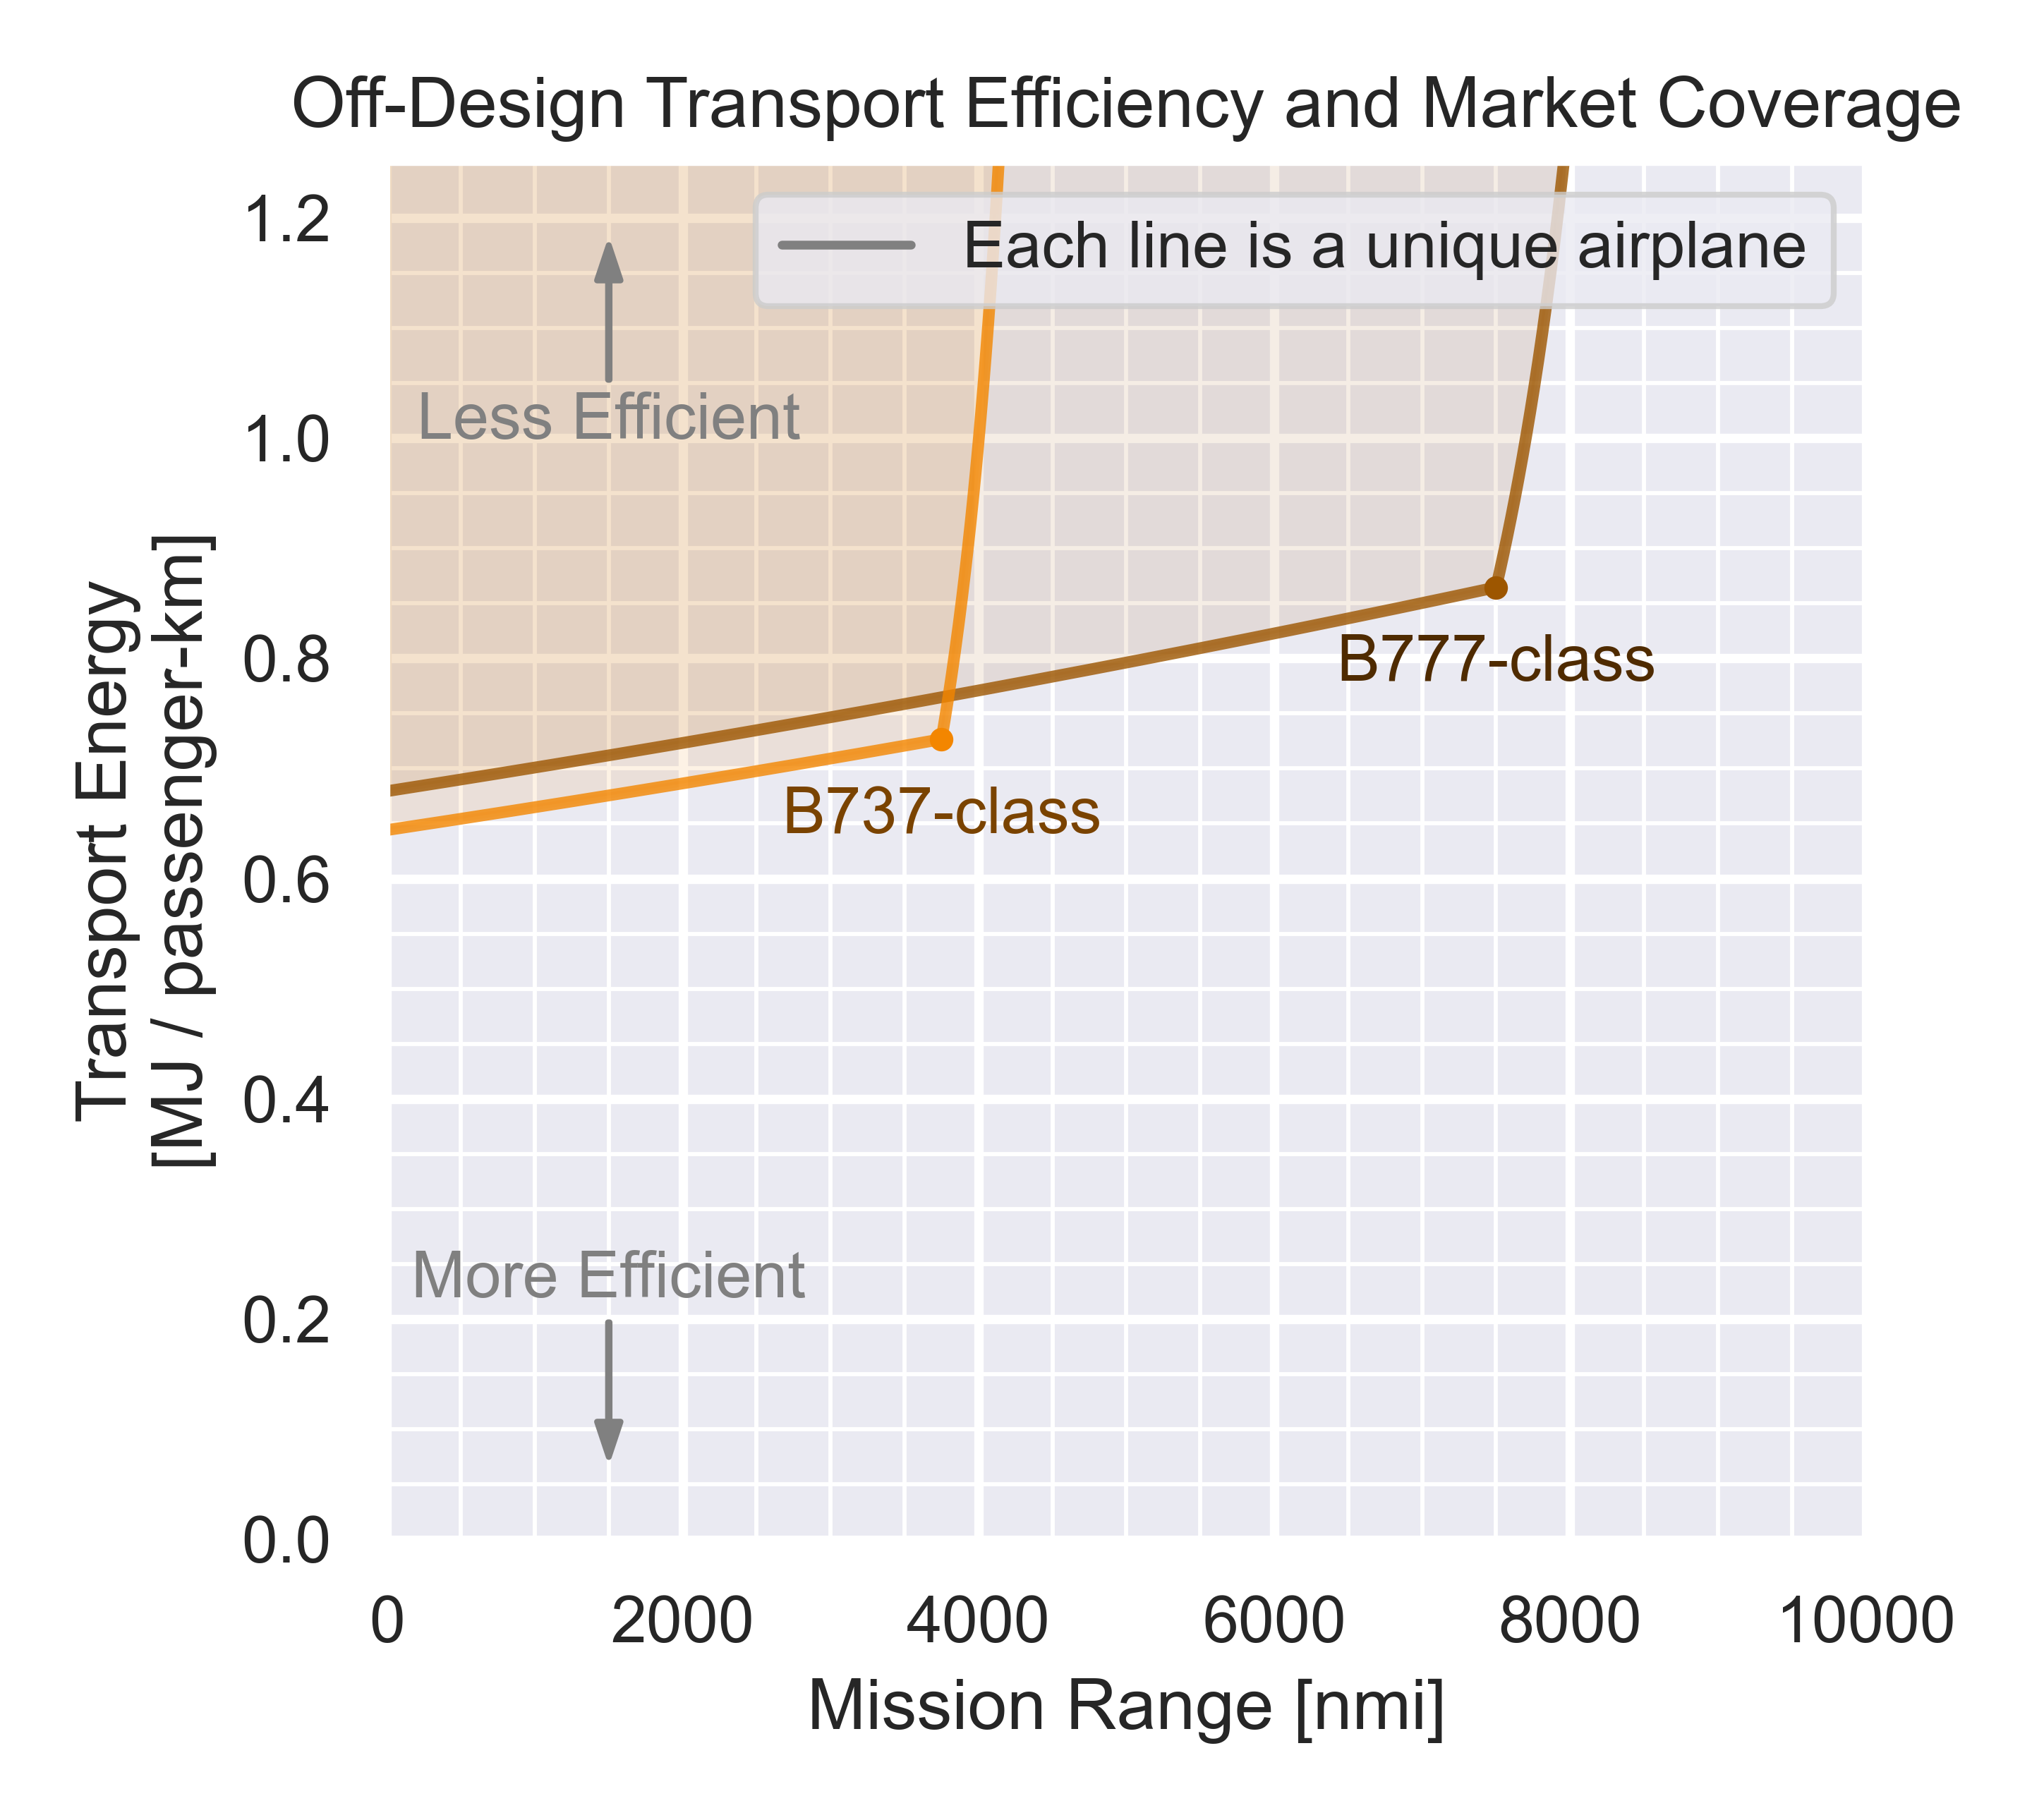
\includegraphics[width=\textwidth]{../figures/Hydrogen/ppt/media/image32.png}
        \caption{\textbf{Kerosene}-fueled aircraft fleet}
        \label{fig:design_space_h2}
    \end{subfigure}
    \begin{subfigure}[b]{0.49\textwidth}
        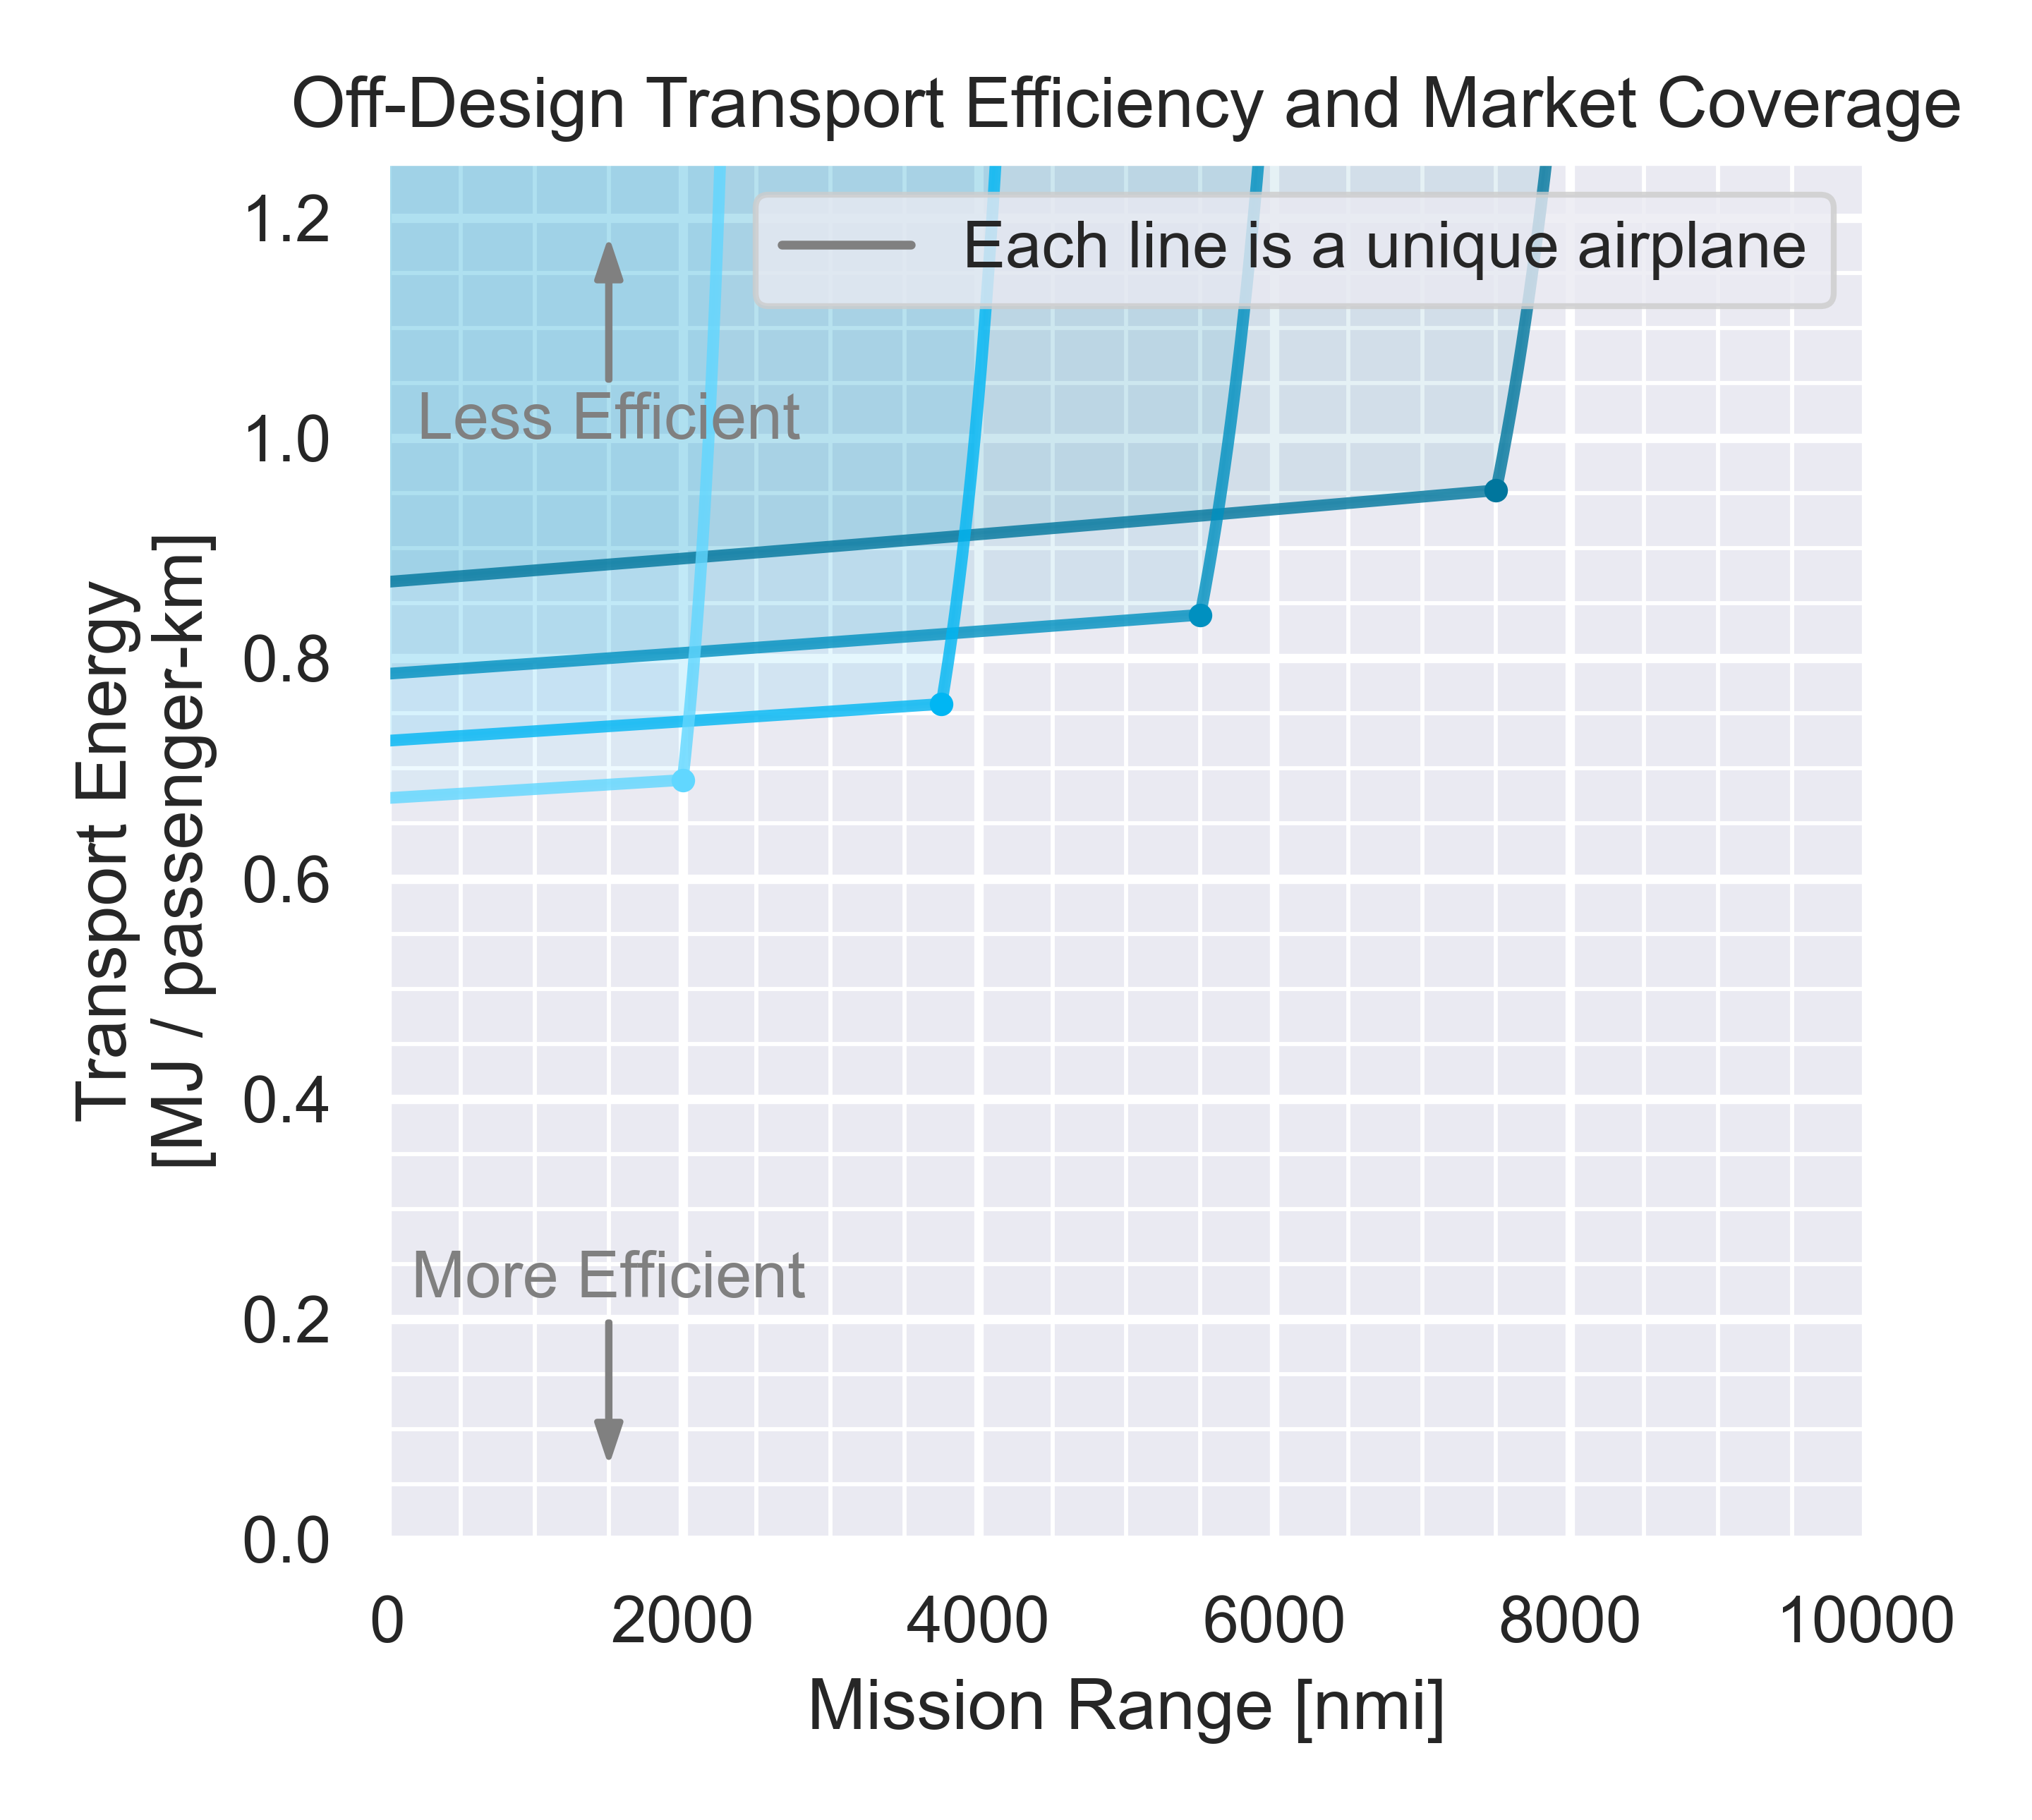
\includegraphics[width=\textwidth]{../figures/Hydrogen/ppt/media/image33.png}
        \caption{\textbf{\lh}-fueled aircraft fleet}
        \label{fig:design_space_kerosene}
    \end{subfigure}
    \caption{These figures show how multiple individual aircraft (each shown by a line) can be combined to cover a market of long-haul flight segments. In general, aircraft will be more fuel-efficient when flown closer to their design range (indicated by a dot on each line). However, hydrogen-fueled aircraft get less benefit from flying shorter-range flights, because their fuel mass fraction is lower. This drives a need for more aviation market segmentation if a hydrogen transportation system is implemented.}
    \label{fig:market_segmentation}
\end{figure}

This is just one example of how a rapid design tool can be used to discover the subtle downstream business-level impacts of a technology choice, which may not be otherwise anticipated. In other cases, this tool can be used to explore the upstream impact of a technology; for example, a study by Gaubatz et al. \cite{gaubatz_estimating_2023} uses this AeroSandbox-based aircraft design tool as one subset of a much broader design study to estimate the grid-level electricity demands of a hydrogen-based long-haul air transportation system.

\subsection{Computational Reproducibility}

A publicly-accessible repository of the hydrogen aircraft design tool is available at \url{https://github.com/peterdsharpe/transport-aircraft}.


\section{Other Aircraft Design Case Studies}

In this final section, we leave brief descriptions and links to other aircraft design case studies that have been conducted using AeroSandbox. While these case studies are not thoroughly described in this document for brevity, they serve to provide more possible starting points for the reader interested in implementing their own aircraft design studies based on the work here.

\subsection{Solar Seaplane}
\label{sec:solar-seaplane}

Another aircraft design project that influenced the development of AeroSandbox was the design of a small-scale solar-electric seaplane, which was performed to support teaching work for MIT 16.821: Flight Vehicle Development. This aircraft design aimed to miniaturize a design for a full-scale recreational ultralight aircraft created by students in MIT 16.82: Flight Vehicle Engineering the prior semester. The goal was to roughly recreate the major elements of this previous vehicle, but at a scale that would allow the students to build and test-fly the aircraft within the scope of one semester. As the intended focus of the class was primarily on building techniques rather than design, we elected to give the students a ``point of departure'' design to jump-start the project.

The design of this aircraft was formulated as an optimization problem in AeroSandbox, which yielded the design illustrated in Figure \ref{fig:solar_surfer_design}. This design was then used as a starting point for the students to build their aircraft, which was successfully flown in a series of test flights at the end of the semester.

AeroSandbox code used to develop this aircraft design is publicly available at \url{https://github.com/peterdsharpe/solar-seaplane-preliminary-sizing}.

\newpage
\begin{figure}[H]
    \centering
    \ifdraft{}{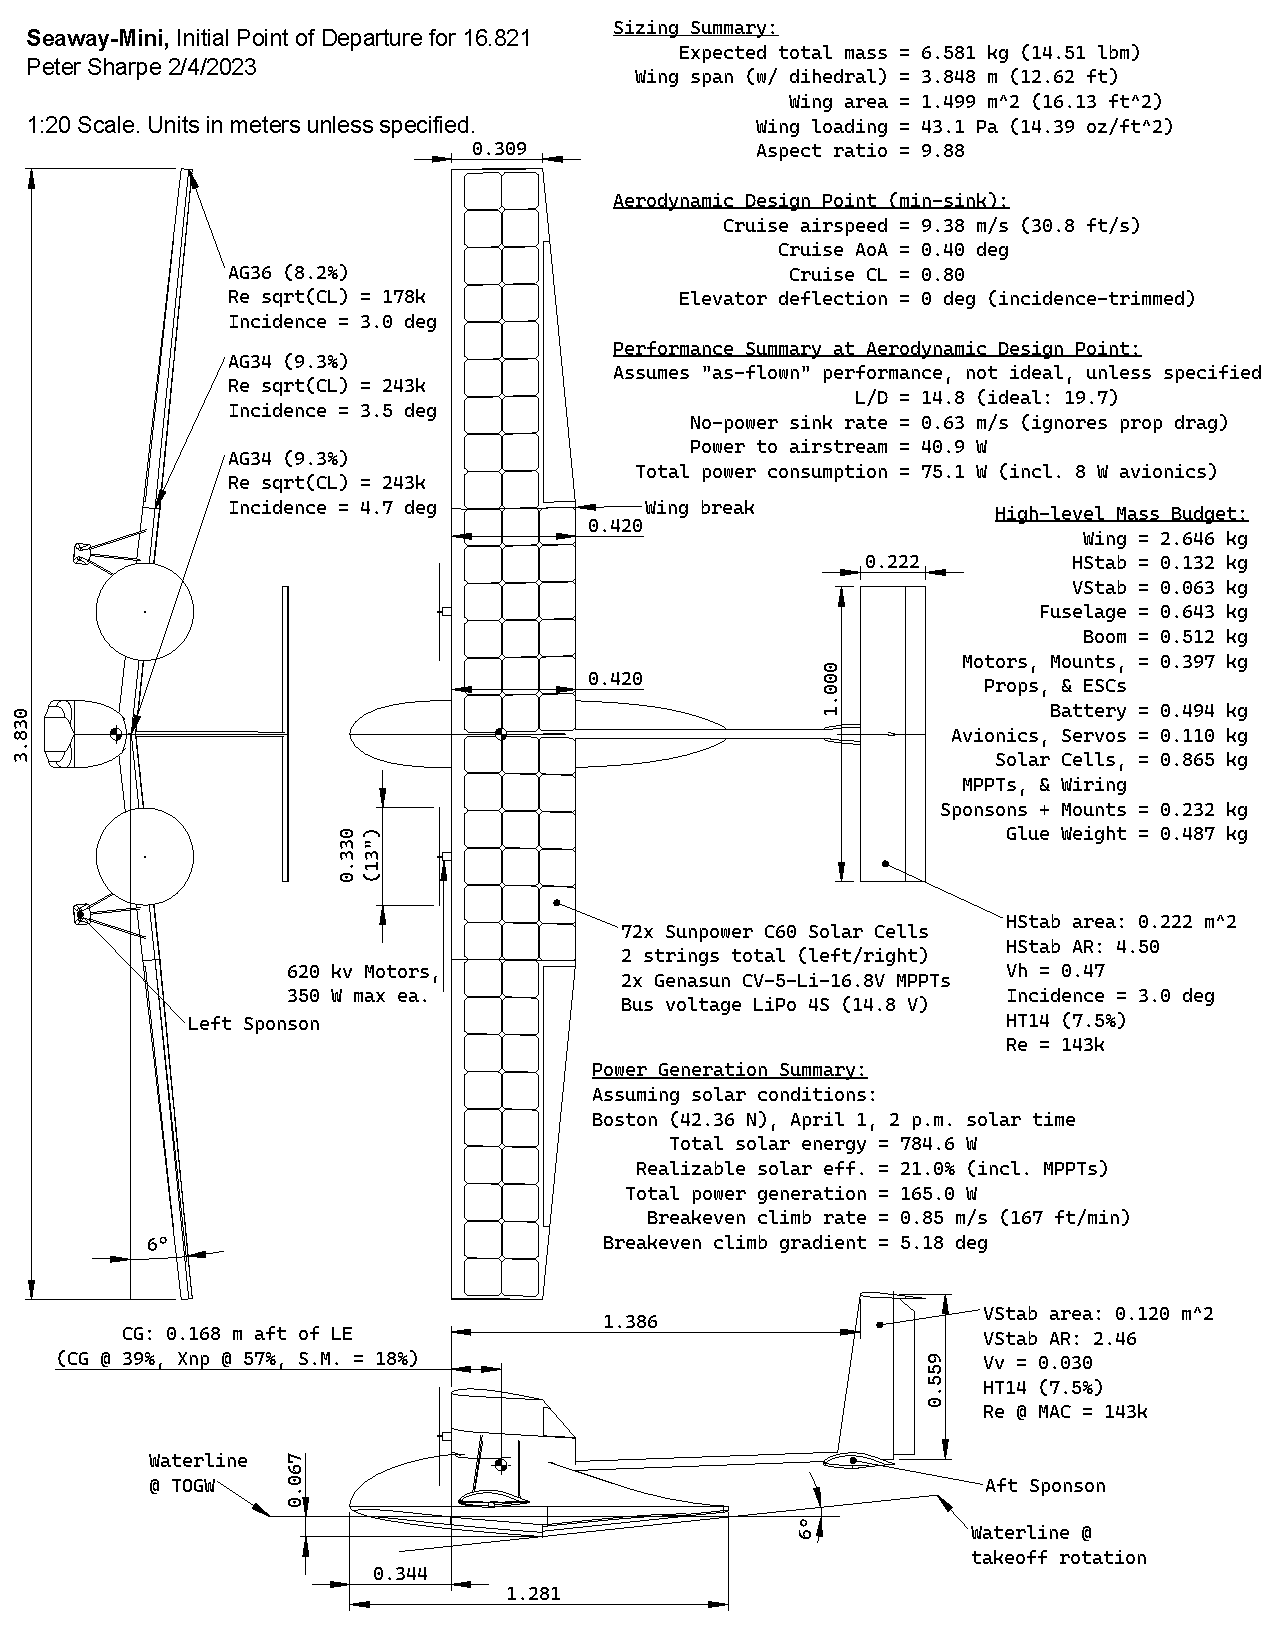
\includegraphics[page=1, width=\textwidth]{../figures/aircraft_sysid/seaway_mini_packet.pdf}}
    \caption{Design drawing of the Solar Surfer solar-electric seaplane.}
    \label{fig:solar_surfer_design}
\end{figure}

\subsection{Feather: Ultra-Lightweight Remote Control Motor-Glider}
\label{sec:feather}

A final aircraft design project that can serve as a useful code example is that of \emph{Feather}, a project to build a minimum-sink-rate 1-meter-wingspan remote-controlled glider. The goal is to be able to exploit even the very weak low-altitude thermals that occur during early morning hours to stay aloft.

Traditionally, remote-control gliders aimed at thermal performance and within this wingspan range have been discus-launch gliders (DLGs). These aircraft are launched by holding the glider by a wingtip, spinning one's entire body in a circle (about the aircraft's yaw axis) and throwing. This achieves very high launch altitudes (up to 70 meters, in extreme cases), which has several benefits:
\begin{itemize}[noitemsep]
    \item Higher launch altitude yields longer flight times (assuming a constant sink rate), and hence more altitude to find thermals.
    \item At higher altitudes, thermals are a) wider, b) stronger\footnote{Particularly for low-altitude thermals, within the atmospheric boundary layer.}, and c) tend to persist longer, which allows for consistent circling once thermals are found.
\end{itemize}

All three combined factors make it easier to consistently stay aloft with thermals once some initial altitude is already achieved. DLGs successfully solve this launch altitude problem, but the violent forces during their launch (often exceeding 30 Gs of acceleration) cause some unfavorable side effects:

\begin{itemize}[noitemsep]
    \item The high launch forces require a heavier wing and tailboom (due to yaw moment during de-rotation immediately after the throw), generally resulting in a higher still-air sink rate.
    \item The design space for tail geometries is constrained by the need to minimize fuselage boom torsion. For example, vertical stabilizers must be roughly top-bottom symmetric about the fuselage boom axis, which means that $C_{l\beta}$ stability that would ordinarily be provided by a top-mounted vertical stabilizer must be provided by a larger wing dihedral angle.
\end{itemize}

However, in recent years, electronics have become so miniaturized that it is now possible to solve this launch altitude problem with a tiny electric propulsion unit, rather than by discus launch. The concept of operations is to ascend to an initial altitude using a brushless motor and propeller, and then shut off the powertrain to glide. (The propeller folds backwards against the fuselage for reduced drag.) The hypothesis is that the mass ``cost'' of this electric propulsion unit is less than the mass cost of the heavier wing and tailboom required for a discus launch. This is the design space that the Feather project aims to explore.

A design optimization problem is formulated with the goal of minimizing the still-air sink rate. General configuration decisions were inspired by the Drela Apogee HLG \cite{drela_apogee_hlg}. The result is the aircraft shown in Figure \ref{fig:feather_design}, which is currently in the process of being built and flown. The glider overall weighs just 62 grams\footnote{equivalent weight to roughly 14 sheets of paper}, which is roughly half the weight of a typical DLG of this wingspan. Much of this weight savings is made possible by the avionics subsystem, which weighs just 15.3 grams but includes a LiPo battery, a brushless motor, an ESC, a 5-inch folding propeller, two linear servos, an IMU and microprocessor for gyro stabilization, and a remote-control radio receiver. Still-air sink rate is estimated to be roughly 0.29 m/s (57 ft/min), which is competitive with the best DLGs of this wingspan.

AeroSandbox code used to develop this aircraft design is publicly available at \url{https://github.com/peterdsharpe/Feather-RC-Glider}.

\newpage
\begin{figure}[H]
    \centering
    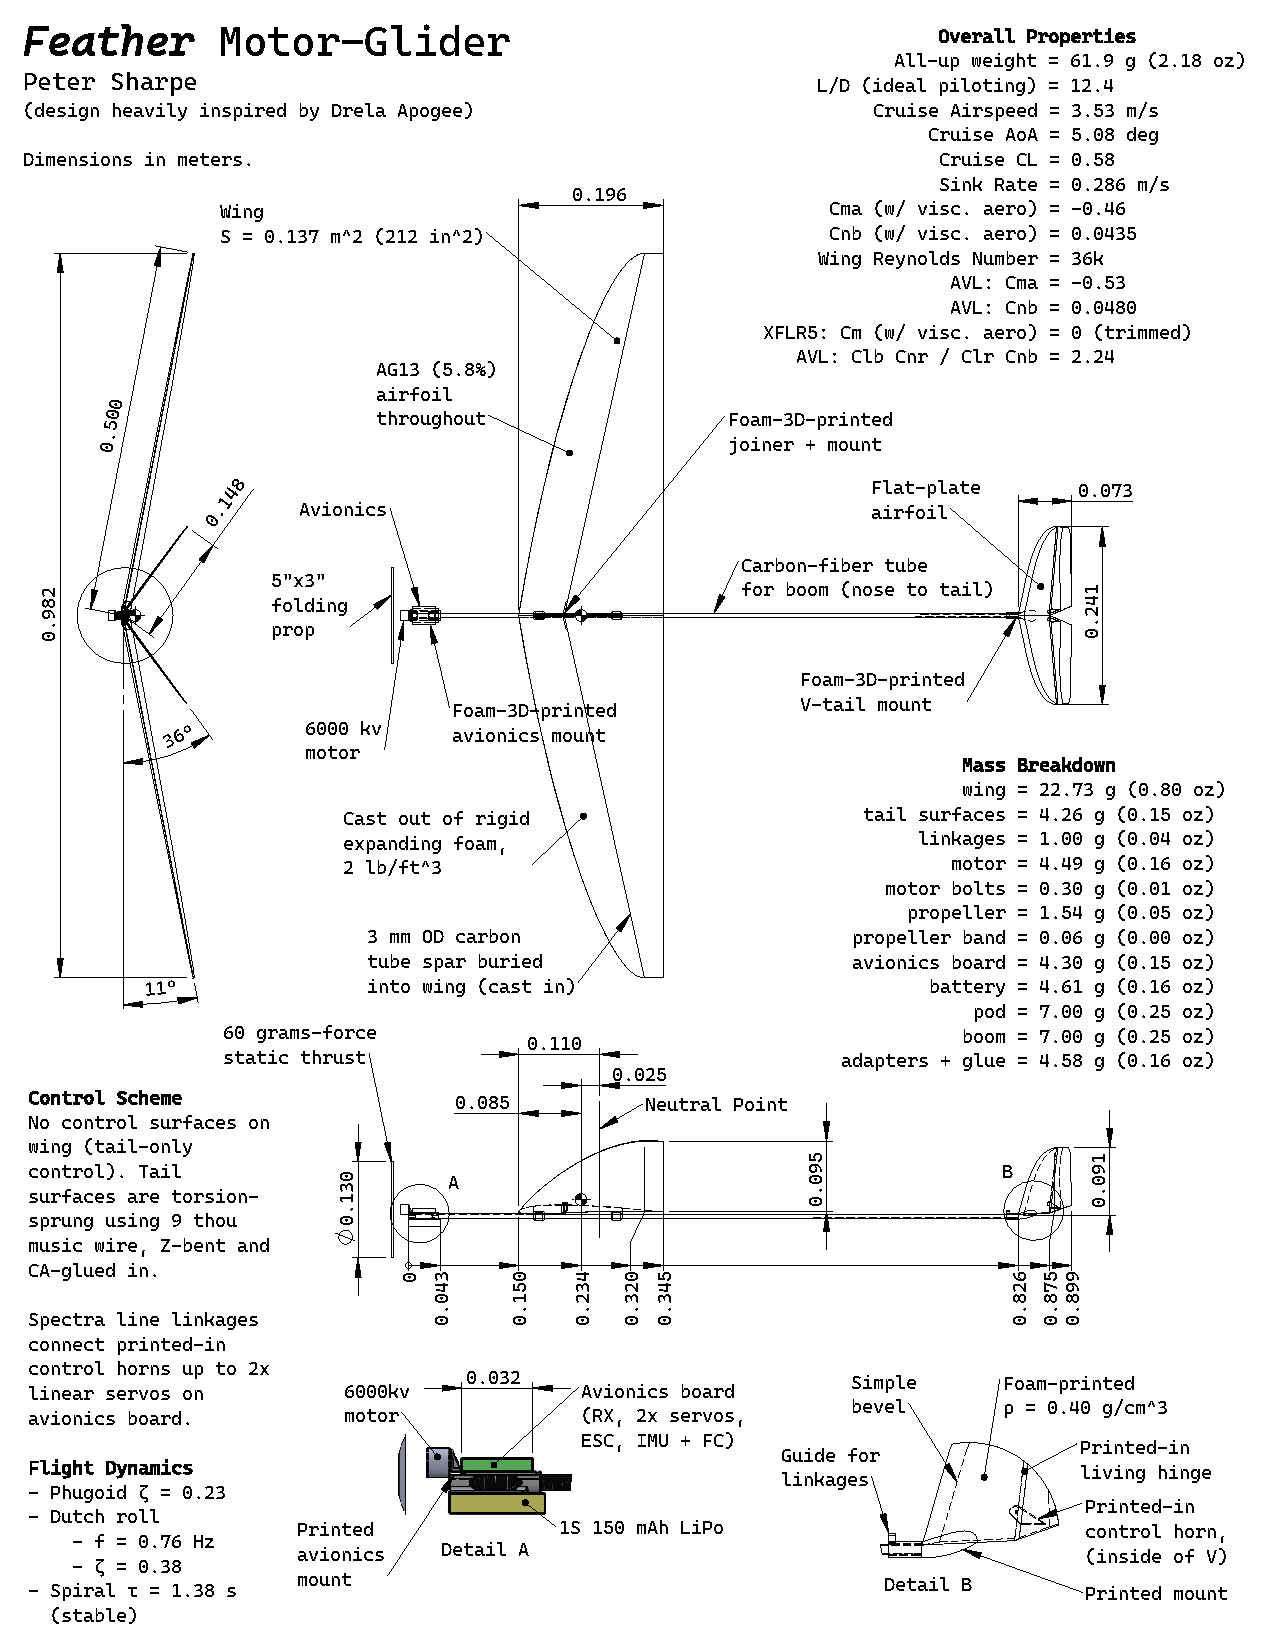
\includegraphics[page=1, width=\textwidth]{../figures/feather.pdf}
    \caption{Design drawing of the Feather ultra-lightweight hand-launched motor-glider.}
    \label{fig:feather_design}
\end{figure}
